
\begin{refsection}
\startcontents[chapters]	
\chapter{Convex analysis}\label{ch:convex-analysis}
\printcontents[chapters]{}{1}{}
\section{Affine sets}
\subsection{Basic concepts}
\begin{definition}[affine sets]\index{affine set}
A set $\subset \R^d$ is affine set if for all $x,y\in X$ and $\lambda, \gamma, \lambda + \gamma = 1$, then $\lambda x + \gamma y \in X$
\end{definition}


\begin{lemma}
Arbitrary intersection of affine sets is an affine set.
\end{lemma}


\begin{definition}[affine combination]\index{affine combination} 
	Given $x,y\in \R^d$, the affine combination $z$ of $x,y$ refers to
	$$z=ax+by,a+b=1$$
\end{definition}


\begin{definition}[affine hull]
The affine hull of $X$ is defined as 
		$$aff(X) = \{\lambda_1 x_1 + ... + \lambda_t x_t: x_1,...,x_t\in X, \sum_i \lambda_i = 1\} $$
		That is, the affine hull the the set of all affine combinations of points in $X$.
\end{definition}

\begin{lemma}[affine hull as the smallest containing affine set]
The affine hull of $X$, denoted as $aff(X)$, is the smallest affine hull containing $X$. Moreover, a set $X$ is affine if $X = aff(X)$.
\end{lemma}




\begin{lemma}[characterization via linear equations]\cite[5]{rockafellar1997convex}\label{ch:convex-analysis:th:affinesetcharacterizationoflinearequation}
\begin{itemize}
\item 	The solution to the linear equation $Ax = 0$ form a linear subspace $X$. Moreover, every linear subspace set can be represented as
	$$\{x: Ax = 0\}$$
\item 	The solution to the linear equation $Ax = b$ form an affine subspace $X$. Moreover, every affine set can be represented as
	$$\{x: Ax = b\}$$	
\end{itemize}
\end{lemma}
\begin{proof}
(1) (a) nullspace is subspace; (b) consider the orthogonal complement $X^\perp$, and let basis of $X^\perp$ be the rows of $A$.
(2) (a)
	Let $x_1,x_2$ be such that $Ax_1 = b,Ax_2 = b$, then
	$$A(ax_1+(1-a)x_2) = ab+(1-a)b = b$$
	therefore $ax_1+ax_2$ is also the solution. Thus the solution form an affine subspace.
	(b) Let $L$ be the associated linear subspace, then consider the orthogonal complement $L^\perp$, and let basis of $L^\perp$ be the rows of $A$. Since $X = L+a$, for some $a\in \R^d$, then $X=\{x:A(x-a)=0\} = \{x:Ax=Aa\}$.
\end{proof}


\begin{definition}[parallel relation in affine sets]\index{parallel affine sets}
An affine set $M$ is said to be \textbf{parallel} to an affine set $L$ if there exist some $a$ such that 
$$M = L + a$$
\end{definition}

\begin{lemma}[translational invariance in affine subspace]
	If $X\subset \R^d$ is an affine subspace, then for every $x_0\in \R^d$, $X-x_0$ is still an affine subspace. That is, affine subspace is translational invariant, and shifted affine subspaces are parallel to each other.
\end{lemma}
\begin{proof}
	Let $x,y \in X$, then $x-x_0,y-x_0 \in X-x_0$, and then we can verify $$a(x-x_0) + b(x-x_0),a+b=1$$ also belongs to $X-x_0$.
\end{proof}


\begin{lemma}[affine subspace to linear subspace]\cite[4]{rockafellar1997convex}
    If an affine subspace $X$ contains 0, then $X$ is also an linear space.
\end{lemma}
\begin{proof}
    (1) closedness under scalar multiplication: Let $x\in X$, then
    $$\lambda x + (1-\lambda) 0 = \lambda x \in X,\forall \lambda \in \F$$
    (2) closedness under addition:
    Let $x,y\in X$, then $x+y = 2(\frac{1}{2}(x+y)) \in X$, since $\frac{1}{2}(x+y)\in X$ and $X$ is closed under scalar multiplication.
    Other properties can be verified easily.
\end{proof}

\begin{lemma}[conversion from affine subspace to linear subspace]
	If $X\subset \R^d$ is an affine subspace, then for every $x_0\in X$, $X-x_0$ is a linear space. Moreover, 
	$$X-x_1 = X-x_2,\forall x_1\neq x_2, x_1,x_2\in X$$
\end{lemma}
\begin{proof}
(1) $X-x_0$ is an affine subspace containing 0.
(2) Let $L_1 = X - x_1$ and $L_2 = X-x_2$, then $L_1 = L_2 + a,a=x_1-x_2$. Then since $L_1$ contains $0$ then $-a \in L_2$, further implying $a\in L_2$, because $L_2 = a+L_2,a\in L_2$ due to closedness of vector space, therefore
$$L_1=L_2$$
\end{proof}


\begin{corollary}[associated unique linear subspace]
Every non-empty affine set $M$ is parallel to a unique linear subspace $L$, which is given as $L=M-x,x\in M$. 
\end{corollary}





\subsection{Affine independence and dimensions}
\begin{definition}[dimension of an affine set]\cite[4]{rockafellar1997convex}
The dimension of an affine set is defined as the dimension of its parallel linear subspace.
\end{definition}


\begin{definition}[affine independence]\index{affine independence}
A set $X$ is affinely independent if there is no $x\in X$ such that $x\in aff(X-\{x\})$. That is, for every element in $X$, it can not be written as affine combination of the others. 
\end{definition}

\begin{definition}[affine independence,alternative]\cite[7]{rockafellar1997convex}
A set $X$ of $m+1$ points $b_0,b_1,...,b_m$ are affinely independent if $aff(X)$ has dimension of $m$; that is the linear subspace 
$$X-b_i,i\in \{0,1,...,m\}$$
has dimension of $m$; or equivalently, the set
$$b_1-b_0,b_2-b_0,...,b_m-b_0$$ are linearly independent.
\end{definition}

\begin{lemma}[algebraic criterion for affine independence]\cite[23]{mordukhovich2013easy} 
	The elements $x_0,...,x_m$ in $\R^n,m \geq 1$, are affinely independent if	and only if
	$$\sum_{i=1}^m \lambda_i v_i = 0,\sum_{i=0}^m \lambda_i = 0 \Rightarrow \lambda_i = 0, \forall i=0,...,m$$
\end{lemma}
\begin{proof}
(1) Suppose 
	$$\sum_{i=0}^m \lambda_i v_i = 0,\sum_{i=0}^m \lambda_i = 0 \Rightarrow \lambda_i = 0, \forall i=0,...,m$$
	We can rewrite as
		$$\sum_{i=1}^m \lambda_i (v_i-v_0) = 0 \Rightarrow \lambda_i = 0, \forall i=1,...,m$$
		which implies $v_i-v_0,i=1,...,m$ are linearly independent. Therefore $v_0,...,v_m$ are affinely independent.
(2) Suppose affinely independent. WLOG, suppose $\lambda_0 \neq 0$, we have
$$\lambda_0 v_0 = -\sum_{i=1}^m \lambda_i v_i$$
add both sides with $\sum_{i=1}^m \lambda_i v_0$, we have
$$ 0 = \sum_{i=1}^m \lambda_i (v_i - v_0)$$
implies $\lambda_i = 0,i=1,...,m \Rightarrow \lambda_0 = 0$, contradicts $\lambda_0 \neq 0$.
\end{proof}



\begin{remark}[linear space analog]
	A set $X$ is linearly independent if every $x\in X$ cannot be written as the linear combination of the others. Or there is no $x\in X$ such that $x\in span(X-\{x\})$
\end{remark}

\begin{theorem}[Barycentric coordinate system]\index{Barycentric coordinate system}\label{ch:convex-analysis:th:affineBaricenteric}
Let $b_0,b_1,...,b_m$ be affinely independent, let $M=aff(b_0,...,b_m)$. Then for any $x\in M$, we have a \textbf{unique affine combination} representation for $x$, given as
$$x = \sum_{i=0}^m a_ib_i,\sum_{i=0}^m a_i = 1,a_i\in \R$$
We can view this as the Barycentric coordinate system.
\end{theorem}
\begin{proof}
Because $b_0,b_1,...,b_m$ be affinely independent, then the set
$$b_1-b_0,...,b_m-b_0$$ are linearly independent. Because $x\in M$, then $x$ has representation of
$$x = \sum_{i=0}^m a_ib_i,\sum_{i=0}^m a_i = 1$$
To show uniqueness, we subtract out $b_0$ on both side, we have
$$x-b_0 = \sum_{i=1}^m a_i(b_i-b_0)$$
Suppose we also have 
$$x-b_0 = \sum_{i=1}^m c_i(b_i-b_0)$$
Then we have 
$$\sum_{i=1}^m (c_i-a_i)(b_i-b_0) = 0$$
implies $c_i=a_i,i=1,2,...,m$ due to linear independence of $b_1-b_0,...,b_m-b_0$.
\end{proof}




\begin{theorem}
	Let $X\subset \R^d$. Then the following are equivalent:
	\begin{itemize}
		\item $X$ is an affinely independent
		\item For every $x\in X$, the set $\{v-x:v\in X-\{x\}\}$ is linearly independent. 
		\item There exists $x\in X$ such that the set $\{v-x:v\in X-\{x\}\}$ is linearly independent.
		\item The set of vectors $\{(x,1)\in \R^{d+1},x\in X \}$ is linearly independent.  
		\item $X$ is finite set with vectors $x_1,...,x_m$ such that $$\lambda_1 x_1 + ... + \lambda_m x_m = 0, \lambda_1+...+\lambda_m = 0$$ implies
		$\lambda_1 =... = \lambda_m = 0$
	\end{itemize}
\end{theorem}
\begin{proof}
\end{proof}
\begin{theorem}
	Let $X\subset \R^d$. The following are equivalent.
	\begin{itemize}
		\item $X$ is an affine subspace
		\item For every $x\in X$, the set $X-x$ is a linear subspace of dimension $0\leq m\leq d$
		\item There exist affinely independent vectors $x_1,...,x_{m+1}$ for some $0 \leq m \leq d$ such that every $x\in X$ can be written as $x = \sum_i\lambda_ix_i,\sum_i\lambda_i = 1$
		\item There exists a matrix $A\in \R^{(d-m)\times d}$ with full row rank and a vector $b\in \R^m$ for some $0\leq m\leq d$ such that $$X=\{x\in \R^d: Ax = b\}$$
	\end{itemize}
\end{theorem}
\begin{proof}
	
\end{proof}


\begin{corollary}
	If $X$ is a set of affine independent points, then $dim(aff(X)) = \abs{X}-1$.($aff(X)$ is the affine hull of $X$.)
\end{corollary}





\subsection{Affine transformations}
\begin{definition}[affine transformation]\cite[7]{rockafellar1997convex}\index{affine transformation}
A single-valued transformation from $T:x\to Tx$ is called affine transformation, if
$$T((1-\lambda)a + \lambda b) = (1-\lambda)Ta + \lambda Tb.$$
\end{definition}


\begin{theorem}[affine transformation vs. linear transformation]\cite[7]{rockafellar1997convex}
The transformations $T:\R^n\to \R^m$ are the affine mappings $T$ if and only if they are in the form $$Tx = Ax + a$$, where $A$ is a linear transformation and $a\in \R^m$
\end{theorem}
\begin{proof}
(1) It is easy to show that $Tx=Ax+a$ is affine. (2) If $T$ is an affine mapping, then let $a = T0$, and $Ax = Tx - a$, then we can show $$A(\lambda x) = T(\lambda x + (1-\lambda) 0) - a =\lambda (Tx - a)$$
and $$A(x + y) = 2A(\frac{1}{2}(x+y)) = 2(\frac{1}{2}(Tx + Ty -2a)) = Tx+Ty - 2a = Ax + Ay$$
therefore, there exists a linear mapping $A$ such that $Tx = Ax + a$.
\end{proof}

\section{Convex sets and cones}\label{ch:convex-optimization:sec:convex-set}
\subsection{Basic concepts}
\begin{definition}[convex set, strictly convex set]\index{convex set}\hfill
\begin{itemize}
	\item 	A set $S$ is said to be a convex set if and only if for any two points $x,y\in S$, we have
	$$\alpha x + (1-\alpha) y \in S,\forall \alpha\in [0,1].$$
	\item 	A set $S$ is said to be a strictly convex set if and only if for any two points $x,y\in S$, we have
	$$\alpha x + (1-\alpha) y \in int S,\forall \alpha\in (0,1),$$
	where $int S$ is the interior of $S$.
\end{itemize}
\end{definition}

\begin{remark}[topological property of convex sets] A convex set can be either open or closed. For example, $(a,b)$ and $[a,b]$ are both convex sets.
\end{remark}

\begin{remark}[strictly convex set vs. convex set]
Consider a set $S = \{(x,y)| x\geq 0, y\geq 0, x + y \leq 1\}$. This set is convex but not strictly convex. Consider $(0,0)$ and $(1,0)$, any point inside the line segment is not in the interior $S$.	
	
\end{remark}

\begin{definition}[hyperplane and halfspace ]\index{hyperplane}\index{halfspace}
Let $a\in \R^d,\delta\in \R$, then the set $H=\{x\in \R^d:\ip{a,x} = \delta\}$ is called hyperplane. The set $H^+=\{x\in \R^d:\ip{a,x} \geq \delta\}$ and $H^-=\{x\in \R^d:\ip{a,x} \leq \delta\}$ are halfspaces. 
\end{definition}

\begin{remark}
Hyperplanes and halfspaces are all convex sets. 
\end{remark}

\begin{definition}[dimensionality of a convex set]
	Let $X$ be a convex set, then $dim(X)$ equals to the maximum number of affinely independent points in $X$.
\end{definition}


\begin{lemma}[preservation of convexity]\label{ch:convex-analysis:th:preservationconvexity}\hfill
	\begin{itemize}
		\item The intersection of \textbf{arbitrary} collection of convex sets $\cap_{i\in I}C_i$ is a convex set.
		\item The image of any linear function $f$ defined on a convex set $X$ is convex.
		\item If $X$ is convex, then the set $aX=\{ax:x\in X\},a\in \R$ is also convex. Particularly, $-X$(the symmetric set with respect to origin) is convex.
		\item If $X,Y$ are convex, then $X+Y$ and $X-Y = X+(-Y)$ is also convex.
	\end{itemize}
\end{lemma}
\begin{proof}
(1)	Let $x,y \in \cap_{i\in I}C_i$, then its convex optimization belongs to any convex set $C_i$, and therefore in $\cap_{i\in I}C_i$.(2)$a f(x) + (1-a) f(y) = f(ax+(1-a)y) \in Im(f)$. (3)(4) directly follow from definition,(4) will use (3).
\end{proof}

\begin{remark}[Empty set is convex]
Note that intersection might result in empty set. Even so, it does not violate above lemma, since empty set is also convex.
\end{remark}


\begin{lemma}
\cite[44]{bertsimas1997introduction}
A convex combination of a finite number of elements of a convex set $X$ also belongs to that set. 
\end{lemma}
\begin{proof} 
Use induction to prove, starting from n=2. Suppose $n=k$ holds, then for $n=k+1$, we have
$$\lambda_0 a_0 + \lambda_1 a_1 + ... + \lambda_k a_k = \lambda_0 a_0 + (1-\lambda_0)(\frac{\lambda_1}{1-\lambda_0}a_1 + ... + \frac{\lambda_k}{1-\lambda_0}a_k) \in X,\sum_i\lambda_i=1$$
since $(\frac{\lambda_1}{1-\lambda_0}a_1 + ... + \frac{\lambda_k}{1-\lambda_0}a_k) \in X$ by assumption.
\end{proof}
 
\begin{theorem}[convex hull as the smallest containing affine set]
The convex hull of $X$, denoted as $conv(X)$,given as
$$conv(X) = \{\lambda_1 x_1 + ... + \lambda_t x_t: x_1,...,x_t\in X,\lambda_1,...,\lambda_t \geq 0, \sum_i \lambda_i = 1\} $$
is the smallest convex hull containing $X$. Moreover, a set $X$ is convex if $X = conv(X)$. 
\end{theorem}
\begin{proof}
It is easy to see $X\subseteq conv(X)$. To prove it is the smallest: let $C$ be any other convex set that containing $X$, then we have $conv(X) \subseteq C$ due to above lemma.
\end{proof}


\begin{lemma}[topological properties of convex set]\cite[94]{hiriart2013convex}
If $C$ is convex, so are its interior $int(C)$ and its closure $cl(C)$.		
\end{lemma} 
\begin{proof}
(1) (informal) let $x_1,x_2\in int(C)$, then there exist open balls  $B_1,B_2 \subset int(C)$ centering on $x_1,x_2$. Let $x_3$ be the convex combination of $x_1,x_2$, then we can always find an open ball centered on $x_3$ with intermediate size that is contained in $int(C)$.(note that every point in $B_2$ will be the convex combination of some pair of points in $B_1,B_2$). (2) Consider two convergent sequence $x^1_n,x^2_n$ in $C$, the convex combination of the two sequence will be in $C$ and $cl(C)$, since $C\subset cl(C)$. Note that the limit point of this new sequence will exist due to the algrabraic property of limits and the limit will be in $cl(C)$ since $cl(C)$ is closed.   
\end{proof}


\subsection{Polytope and simplex}
\begin{definition}[polytope]\index{polytope}\cite[12]{rockafellar1997convex}
A set which is the convex hull of finitely many points is called a polytope.
\end{definition}

\begin{definition}[simplex]\index{simplex}\cite[12]{rockafellar1997convex}
If the $m+1$ points $\{b_0,b_1,...,b_m\}$ are affinely independent, then its convex hull is called \textbf{m-dimensional simplex}.
\end{definition}


\begin{theorem}[Barycentric coordinate system in simplex]
Every point $x$ in a simplex constructed from affinely independent points $\{b_0,b_1,...,b_m\}$ can be \textbf{uniquely expressed as}
$$x = \sum_{i=0}^m \lambda_i b_i, \sum_{i=0}^m \lambda_i = 0,\lambda_i \geq 0$$
\end{theorem}
\begin{proof}
see \autoref{ch:convex-analysis:th:affineBaricenteric}.
\end{proof}


\subsection{Cones}

\begin{definition}[cone]\index{cone}
	A subset $K \subset \R^n$ is called a cone if for every $x\in K$ and all $a \geq 0$, $ax\in K$.
\end{definition}

\begin{mdframed}
	\textbf{Caution!}\\
	A cone is not necessarily a convex set. For example, the union of the first quadrant and third quadrant is a cone, but it is non-convex.
\end{mdframed}


\begin{definition}[convex cone]\index{convex cone}
	A subset $K \subset \R^n$ is called a convex cone if it is convex and it is a cone. A convex cone $X$ can also be defined as
	$\forall x,y\in X,\lambda,\gamma \geq 0, \lambda x + \gamma y \in X$.	
\end{definition}

\begin{example}[convex cones]
\begin{itemize}
\item The subspaces in $\R^n$ are trivial convex cones.
\item The non-negative orthant of $\R^m$:
$$\{x=(x_1,...,x_m):x_1 \geq 0,...,x_m \geq 0\}$$
\end{itemize}
\end{example}

\begin{definition}[convex cone]\index{convex cone}
\cite[lec 1]{Basu2016introduction}\cite[14]{rockafellar1997convex}
A set $\subset \R^d$ is convex cone if for all $x,y\in X$ and $\lambda, \gamma \geq 0$, then $\lambda x + \gamma y \in X$; that is a convex cone is set closed under addition and nonnegative scalar multiplication.
\end{definition}


\begin{definition}[conical hull]\cite[lec 1]{Basu2016introduction}\index{conical hull}
The conical hull of $X$ is defined as 
		$$cone(X) = \{\lambda_1 x_1 + ... + \lambda_t x_t: x_1,...,x_t\in X,\lambda_1,...,\lambda_t \geq 0\} $$
\end{definition}

\begin{lemma}\hfill
A set $X$ is a cone if $X = cone(X)$(i.e. the conic hull of $X$); that is $cone(X)$ is the smallest conic hull containing $X$.
\end{lemma}
\begin{proof}
See proofs in affine set and convex set sections.
\end{proof}




\subsection{An unified framework}

\begin{definition}[convex set, convex cone, affine set, linear set]\hfill \index{convex set}\index{convex cone}\index{affine set}\index{linear set}
\cite[lec 1]{Basu2016introduction}
\begin{itemize}
	\item A set $\subset \R^d$ is convex if for all $x,y\in X$ and $\lambda, \gamma \geq 0, \lambda + \gamma = 1$, then $\lambda x + \gamma y \in X$
	\item A set $\subset \R^d$ is convex cone if for all $x,y\in X$ and $\lambda, \gamma \geq 0$, then $\lambda x + \gamma y \in X$
	\item A set $\subset \R^d$ is affine set if for all $x,y\in X$ and $\lambda, \gamma, \lambda + \gamma = 1$, then $\lambda x + \gamma y \in X$
	\item A set $\subset \R^d$ is convex if for all $x,y\in X$ and $\lambda, \gamma \geq 0, \lambda + \gamma = 1$, then $\lambda x + \gamma y \in X$
\end{itemize}
\end{definition}	




\begin{lemma}
convex cone, affine set and linear set are all convex sets
\end{lemma}
\begin{proof}
	Since convex 
	sets have the most restrict requirement on $\lambda,\gamma$, therefore,convex cone, affine set and linear set are all convex sets. 
\end{proof}

\begin{lemma}
The arbitrary intersection of convex cones/affine sets/linear sets/convex sets are convex cones/affine sets/linear sets/convex sets.
\end{lemma}
\begin{proof}
	Straight forward.
\end{proof}




\begin{definition}[convex hull, conical hull, affine hull, linear hull]\cite[lec 1]{Basu2016introduction}\index{convex hull}\index{conical hull}\index{affine hull}\index{linear hull}\hfill
	\begin{itemize}
		\item The convex hull of $X$ is defined as 
		$$conv(X) = \{\lambda_1 x_1 + ... + \lambda_t x_t: x_1,...,x_t\in X,\lambda_1,...,\lambda_t \geq 0, \sum_i \lambda_i = 1\} $$
		\item The conical hull of $X$ is defined as 
		$$cone(X) = \{\lambda_1 x_1 + ... + \lambda_t x_t: x_1,...,x_t\in X,\lambda_1,...,\lambda_t \geq 0\} $$
		\item The affine hull of $X$ is defined as 
		$$aff(X) = \{\lambda_1 x_1 + ... + \lambda_t x_t: x_1,...,x_t\in X, \sum_i \lambda_i = 1\} $$
		\item The linear hull of $X$ is defined as 
		$$span(X) = \{\lambda_1 x_1 + ... + \lambda_t x_t: x_1,...,x_t\in X,\lambda_1,...,\lambda_t \in \R\} $$
	\end{itemize}
\end{definition}

\begin{lemma}
	Given a set $X$, then we have
	$$conv(X)\subset cone(X) \subset span(X)$$
	$$conv(X)\subset affine(X) \subset span(X)$$
\end{lemma}
\begin{proof}
	Directly from definitions.
\end{proof}

\begin{lemma}\hfill
	\begin{itemize}
		\item A set $X$ is convex  if $X = conv(X)$(i.e. the convex hull of $X$); that is $conv(X)$ is the smallest convex hull containing $X$.
		\item A set $X$ is a cone if $X = cone(X)$(i.e. the conic hull of $X$); that is $aff(X)$ is the smallest conic hull containing $X$.
		\item A set $X$ is affine if $X = aff(X)$(i.e. the affine hull of $X$); that is $aff(X)$ is the smallest affine hull containing $X$.
		\item A set $X$ is a linear space if $X = span(X)$(i.e. the linear hull of $X$); that is $span(X)$ is the smallest linear hull containing $X$.
	\end{itemize}
\end{lemma}
\begin{proof}
See proofs in affine set and convex set sections.
\end{proof}

\section{Projection theorems}
\begin{definition}[projection onto a convex set]\index{projection onto a convex set}
Let $\cX \subseteq \R^n$ be a nonempty closed convex set. The projection of a given vector $y\in \R^n$ onto $\cX$ is
$$Proj_\cX(y) = \arg\min_{x\in\cX} \norm{x-y}_2.$$ 
\end{definition}



\begin{theorem}[projection theorem for convex set]\cite[19]{bertsekas2016nonlinear}\label{ch:convex-analysis:th:projectionconvexset}
Let $\cX$ be a closed convex set in $\R^n$, let $\norm{.}$ be the Euclidean norm. Then, we have
\begin{itemize}
	\item For every $x\in \R^n$, the following optimalization problem
	$$\min_{y\in X}\norm{y-x}^2$$
	has an unique global minimum solution $x^*$.
	\item (obtuse angle theorem) $x^* = Proj_\cX(y), y\in\R^n$ is the unique global minimum if and 
	only if $$(y-x^*)^T(x-x^*) \leq 0,\forall x\in \cX$$
	\item The projection mapping $Proj_\cX(y):\R^n\to \cX$ is continuous and non-expansive mapping, i.e. 
	$$\norm{Proj_\cX(y_1)-Proj_\cX (y_2)} \leq \norm{y_1-y_2}.$$
\end{itemize}
\end{theorem}
\begin{proof}
(1) For every $x\in \cX$, it is easy to see that the function $f(y) = \norm{y-x}^2$ is coercive in the set $\cX$. Therefore, from \autoref{ch:calculus:th:WeierstrassCoerciveFunc}, we have at least one global minimizer in $\cX$. This minimizer will be unique (\autoref{ch:convex-optimization:th:uniqueglobalminimumUnderStrictConvexity}) since $f(y) = \norm{y-x}^2$ is strictly convex(The Hessian is positive definite matrix). \\
(2) Use the first order necessary and sufficient condition for $f(x)$ (\autoref{ch:convex-optimization:sec:optimality-conditions})gives
$$\nabla f^T(x-x^*) \geq 0,\forall x\in \cX \Leftrightarrow (x-x^*)^T(x^*-y) \geq 0,\forall x\in \cX$$
(3) 
From (2), we have
\begin{align*}
(y_1 - Proj_\cX(y_1))^T(x - Proj_\cX(y_1))&\leq 0,\forall x\in \cX \\
\implies
(y_1 - Proj_\cX(y_1))^T(Proj_\cX(y_2) - Proj_\cX(y_1))&\leq 0,\forall x\in \cX \\
(y_2 - Proj_\cX(y_2))^T(Proj_\cX(y_1) - Proj_\cX(y_2))&\leq 0,\forall x\in \cX
\end{align*}
Add together, we have
\begin{align*}
-(Proj_\cX(y_1) - Proj_\cX(y_2))^T(y_1 - y_2 - (Proj_\cX(y_1) - Proj_\cX(y_2)))&\leq 0 \\
\norm{Proj_\cX(y_1)-Proj_\cX (y_2)}^2 \leq (Proj_\cX(y_1) - Proj_\cX(y_2))^T(y_1-y_2) &\leq  \norm{Proj_\cX(y_1)-Proj_\cX (y_2)}\norm{y_1-y_2}
\end{align*}
where we use the Cauchy inequality.

Nonexpansiveness directly implies continuity: as $y_1\to y_2$, $Proj_\cX(y_1) \to Proj_\cX(y_2)$.
\end{proof}






\begin{theorem}[generalization to Hilbert space]\cite[69]{luenberger1969optimization}
	Let $x$ be a vector in a Hilbert space $H$ and let $K$ be a closed convex subset of $H$. Then there is an unique vector $k_0 \in K$ such that 
	$$\norm{x-k_0} \leq \norm{x - k} \forall x\in K $$
	Furthermore, a necessary and sufficient condition that $k_0$ be the unique minimizing vector is $\ip{x-k_0,k-k_0} \leq 0, \forall k\in K$.
\end{theorem}




\section{Separation theorems}


\subsection{separating hyperplane theorem}
\begin{theorem}[separating hyperplane theorem]\cite[170]{bertsimas1997introduction}\index{separating hyperplane theorem}\label{ch:convex-analysis:th:separatinghyperplane}
Let $C\subset \R^d$ be a closed convex set and let $x\in\R^d, \notin C$. Then there exists a halfspace that contain $C$ and does not contain $x$. More precisely, there exists $a\in \R^d, \delta \in \R$ such that $\ip{a,y} \leq \delta$ for all $y\in C$ and $\ip{a,x} > \delta$; that is 
$$\ip{a,x} > \ip{a,y},\forall y\in C;$$
or equivalently,
$$\ip{a,x} > \sup_{y\in C}\ip{a,y}.$$
\end{theorem}
\begin{proof}
(1) If $C$ is empty, then any halfspace that does not contain $x$ will suffice. (2) If $C$ is empty, consider a closed ball $B(x,r)$,where $r = \norm{x-\bar{x}},\bar{x}\in C$, then the set $B(x,r)\cap C$ is a closed and compact set, and therefore there exists $x^*$ as the minimizer of problem $\min_{y\in C\cap B}\norm{y-x}$. Let $a = x-x^*$, then from obtuse angle theorem(projection theorem)\autoref{ch:convex-analysis:th:projectionconvexset} for convex set, we have
$$\ip{y-x^*,x-x^*} \leq 0$$
which implies
$$\ip{y-x^*,a}\leq 0 \Leftrightarrow \ip{a,y} \leq \ip{a,x^*} < \ip{a,a + x^*} = \ip{a,x}$$
\end{proof}


\begin{corollary}[separating hyperplane theorem for convex bodies] Let $C_1$ and $C_2$ be two convex subsets in $\R^n$. If $C_1$ and $C_2$ are disjoint, then there exists $a\in \R^n$ such that
	$$\ip{a,x_1}\leq \ip{a,x_2},\forall x_1\in C_1,x_2\in C_2$$ 
\end{corollary}
\begin{proof}
	Consider the convex set $C = C_1 + (-C_2)$ (see \autoref{ch:convex-analysis:th:preservationconvexity}). Since $C$ does not contain origin, from \autoref{ch:convex-analysis:th:separatinghyperplane}, there exists $a\in \R^m,\delta \in \R^m$ such that $$\ip{a,x} \leq \ip{a,0} = 0 \Rightarrow \ip{a,x_1-x_2} \leq 0,\forall x_1\in C_1,x_2\in C_2$$ 
\end{proof}

\begin{figure}[H]
\centering
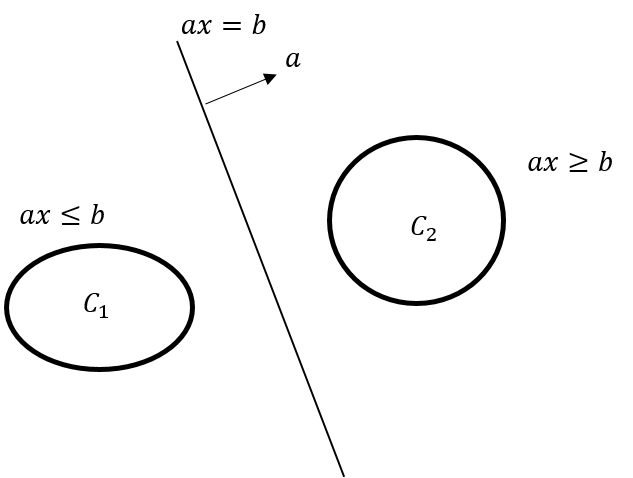
\includegraphics[width=0.5\linewidth]{figures/optimization/separingHyperplaneTheoremDemo}
\caption{An illustration of separating hyperplane theorem for two convex bodies.}
\label{fig:separingHyperplaneTheoremDemo}
\end{figure}


\begin{corollary}
	For every closed convex set $X\subseteq \R^d$ there exists a family of tuples $(a^i,\delta^i),a^i\in \R^d,\delta^i\in \R, i\in I$(where $I$ may be an uncountable index set) such that $X = \cap_{i\in I} H^{-}(a^i,\delta^i)$. In otherwise, every closed convex set can written as the intersection of some family of halfspaces.
\end{corollary}


\begin{corollary}
Every closed convex set $C$ can e written as the intersection of some family of halfspaces.
\end{corollary}
\begin{proof}
Consider all the points $x_i$ outside $C$, then based on separating hyperplane theorem, there exists an halfspaces $H^-(a_i,\delta_i)$, such that $C\subseteq H^-(a_i,\delta_i)$. The intersection of all such halfspaces will be $C$ since every point outside $C$ will not be included in the intersection.
\end{proof}

\begin{definition}[supporting hyperplane]
Given a set $C\subseteq \R^n$. If a vector $x_0$ belongs to $cl(C)$, a hyperplane with parameter $a\in \R^n,\delta\in R$ such that
$$\ip{a,x}\leq \delta, \ip{a,x_0}=\delta$$
is called a supporting hyperpalne for $C$.
\end{definition}

\begin{theorem}[supporting hyperplane theorem]\index{supporting hyperplane theorem}\cite[67]{bertsekas2009convex}
	Let $C\subseteq \R^d$ be a convex set and let $x\in bd(C)$ (the boundary of $C$). Then there exists $a\in\R^d, \delta\in \R$ such that 
	\begin{itemize}
		\item $\ip{a,y}\leq \delta$ for all $y\in C$; that is, $C\subseteq H^-(a,\delta)$
		\item $\ip{a,x} = \delta$
	\end{itemize}
	The hyperplane $\{y\in \R^d:\ip{a,y} = \delta\}$ is called a supporting hyperplane for $C$ at $x$.
\end{theorem}
\begin{proof}
	TODO	
\end{proof}


\subsection{Farka's lemma}
\begin{theorem}[Farkas's lemma, analog in linear equation theory]
	Let $A\in \R^{m\times d}$ and $b\in \R^m$. Exactly one of the following is true:
	\begin{itemize}
		\item $Ax = b$ has a solution
		\item There exists $u\in \R^m$ such that $A^Tu = 0$ and $u^Tb\neq 0$
	\end{itemize}
\end{theorem}
\begin{proof}
(1) If $Ax=b$ has a solution, then $b\in \cR(A)$. Suppose there exists a $u$ such that $A^Tu = 0$, which implies $u\in \cN(A^T)$. Since $b\in \cR(A),u\in \cN(A^T),\cR(A)\perp \cN(A^T)$, it is impossible to have $u^Tb\neq 0$; \\
(2) If $A^Tu = 0$ has a solution $u$ and $u^Tb \neq 0$. Then $b$ has nonzero component in $\cN(A^T)$, and therefore $b$ cannot lie in the $\cR(A)$.
\end{proof}



\begin{theorem}[Farkas' lemma]\index{Farkas' lemma}\label{ch:convex-analysis:th:Farkaslemma}
Let $A\in \R^{m\times d}$ and $b\in \R^m, b\neq 0$. Exactly one of the following is true:
\begin{itemize}
	\item $Ax = b,x\geq 0$ has a solution.
	\item There exists $u\in \R^m$ such that $A^Tu \leq 0$ and $u^Tb > 0$.
\end{itemize}

Or equivalently, exactly one of the following sets must be empty
\begin{itemize}
	\item $\{x|Ax = b, x\geq 0 \}$.
	\item $\{u|A^Ty\leq 0, b^Ty > 0\}$.
\end{itemize}

\end{theorem}
\begin{proof}
(1) Suppose $Ax=b,x\geq 0$ holds, then we suppose that there exists $u\in \R^m$ such that $A^Tu \leq 0$. Multiply $x^T$, we have $(Ax)^Tu \leq 0 \Rightarrow b^Tu \leq 0$, which contradicts $u^Tb > 0$. Therefore, when the first case holds, the second case cannot hold at the same time.
(2) We can view each column $a_i$ of $A$ is a point in $\R^m$, then the set $C = \{y=Ax,x\geq 0\}$ form a cone. $Ax=b,x\geq 0$ has a solution can be interpreted as $b$ is lying in the cone. Suppose $b$ lying outside the cone, then use \autoref{ch:convex-analysis:th:separatinghyperplane} we know that there exists $u\in \R^m,\delta \in \R$ such that
$$\ip{y,u}\leq \delta, \forall y\in C, \ip{u,b} > \delta$$

Also, $0$ is in the cone, we have $\delta \geq 0$, therefore $\ip{u,b} > 0$. To show $\ip{a_i,u}\leq 0,\forall i$, suppose there exist some  $\ip{a_i,u} > 0$, then there exists some scalar $\lambda > 0$ (we can always choose $\lambda$ large enough) such that $\lambda \ip{a_i,u} > \delta$, then $\ip{\lambda a_i,u} > \delta$, contradicting the fact that every point in $C$ satisfying $\ip{\lambda a_i,u} \leq \delta$. Therefore, $\ip{a_i,u}\leq 0,\forall i$
\end{proof}

\begin{figure}[H]
\centering
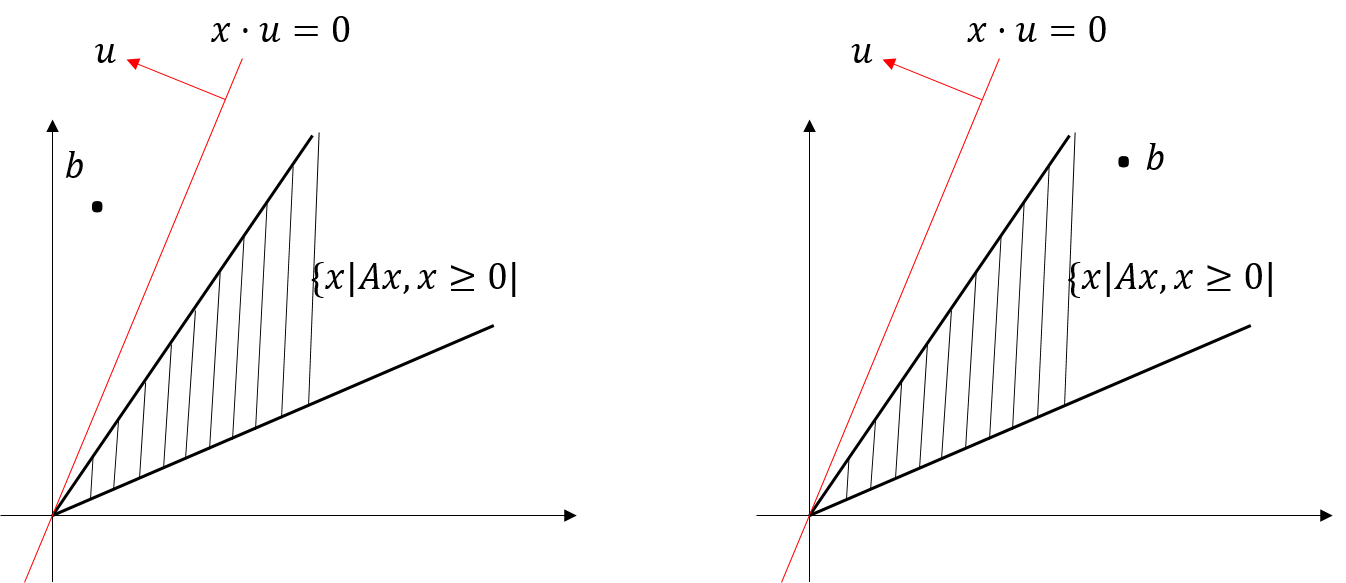
\includegraphics[width=0.7\linewidth]{figures/optimization/FarkasLemmaDemo}
\caption{An illustration of Farkas' lemma. (left) When $b$ lies outside the cone (that is, $Ax = b, x\geq 0$ has no solution), there exists a hyperplane, characterized by normal vector $y$, seperating $b$ and the cone. (right) When $b$ lies inside the cone (that is, $Ax = b, x\geq 0$ has a solution), there does not exist a hyperplane, characterized by normal vector $y$, seperating $b$ and the cone. }
\label{fig:FarkasLemmaDemo}
\end{figure}

\begin{corollary}[Farkas' lemma variant]\index{Farkas' lemma}\label{ch:convex-analysis:th:FarkaslemmaVariant}
	Let $A\in \R^{m\times d}$ and $b\in \R^m, b\neq 0$. Exactly one of the following is true:
	\begin{itemize}
		\item $Ax = b,x > 0$ has a solution.
		\item There exists $u\in \R^m$ such that $A^Tu \leq 0$ and $u^Tb > 0$ (or $A^Tu < 0$ and $u^Tb \geq 0$).
	\end{itemize}
\end{corollary}


\begin{figure}[H]
	\centering
	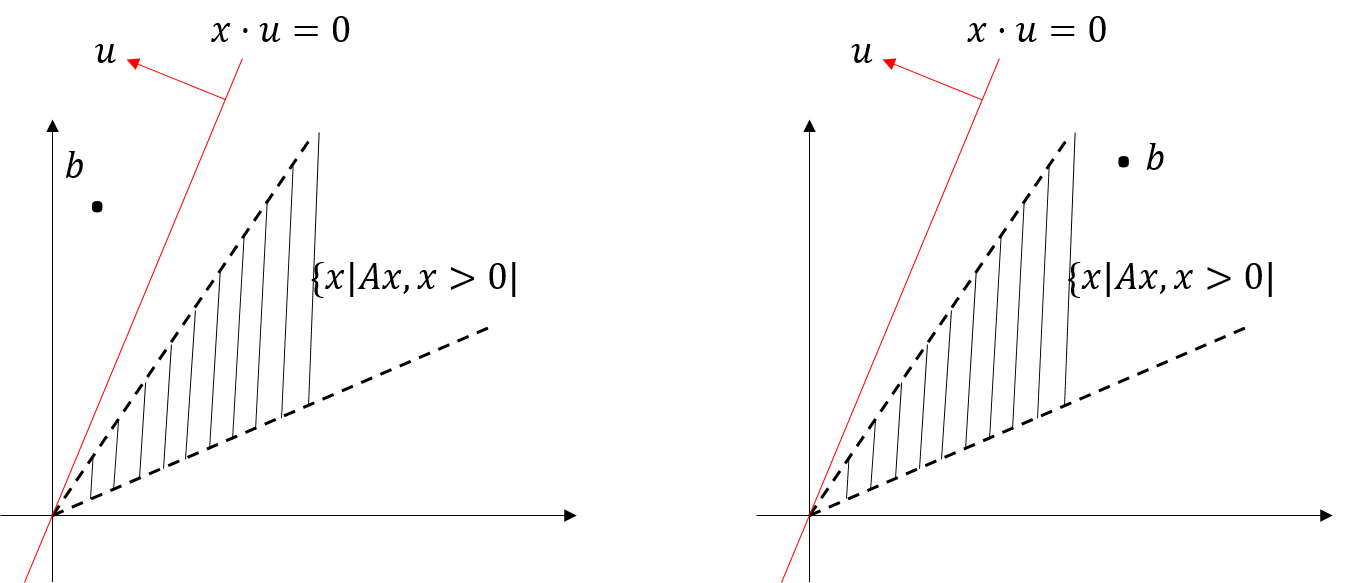
\includegraphics[width=0.7\linewidth]{figures/optimization/FarkasLemmaDemo2}
	\caption{An illustration of Farkas' lemma variant where the cone is open set. (left) When $b$ lies outside the cone (that is, $Ax = b, x> 0$ has no solution), there exists a hyperplane, characterized by normal vector $y$, seperating $b$ and the cone. (right) When $b$ lies inside the cone (that is, $Ax = b, x> 0$ has a solution), there does not exist a hyperplane, characterized by normal vector $y$, seperating $b$ and the cone. }
\end{figure}

\begin{remark}[financial application]
Farkas' lemma in no-arbitrage pricing can be found in \cite[168]{bertsimas1997introduction}.
\end{remark}


\section{Polar set}
\begin{definition}[Polar]\index{polar}
Let $X\in \R^d$ be any set. The set defined as
$$X^\circ = \{y\in \R^d: \ip{y,x}\leq 1,\forall x\in X\}$$
is called the polar of $X$.
\end{definition}

\begin{theorem}
	Let $X\in \R^d$ be any set. Then the following are all true:
	\begin{itemize}
		\item $X^\circ$ is closed, convex set for any $X\subseteq \R^d$(not necessarily convex)
		\item $(X^\circ)^\circ = cl(conv(X\cup \{0\}))$. In particular, if $X$ is a closed convex set containing the origin, then $(X^\circ)^\circ = X$
		\item If $X$ is a linear subspace, then $X^\circ = X^\perp$
		\item If $X$ is a convex cone, then $X^\circ = \{y\in \R^d: \ip{y,x}\leq 0, \forall x\in X\}$
	\end{itemize}
\end{theorem}
\begin{proof}
	(1);(2);(3) Let $z\in X^\perp$, then $\ip{z,x} = 0$ implies $X^\perp \subseteq X^\circ$. For any $y\in R^d$, we can decompose uniquely as $y = y_1 + y_2,y_1\in X,y_2\in X^\perp$. It can be showed that $y_1$ has to be 0 otherwise we can choose $x\in X$ to make $\ip{y,x} = \ip{y_1,x}$ to be arbitrarily large. Therefore, $X^\perp \subset X^\perp$. \\
	(4)
\end{proof}

\begin{remark}
	Polar is a generalization of the orthogonal complement in linear subspace.
\end{remark}


\begin{definition}[polyhedron]\index{polyhedron}
	A finite intersection of halfspaces is called a polyhedron. A polyhedron $P$ can usually be written as
	$$P=\{x\in \R^d, Ax \leq b, A\in \R^{m\times n},b\in \R^n\}$$
	representing the intersection of $m$ halfspaces.
\end{definition}

\begin{remark}
	The unit ball in standard Euclidean norm in $\R^d$ is not a polyhedron because it cannot be represented as finite intersection of halfspaces.
\end{remark}


\section{Extreme subsets}
\begin{definition}[face as an extreme subset]\index{face}\index{extreme subset}
Let $C$ be a convex set. A \textbf{convex subset} $F\subseteq C$ is called an \textbf{extreme subset or a face} of $C$, if for any $x\in F$ the following holds: $x_1,x_2 \in C, \frac{1}{2}(x_1+x_2) = x$ implies that $x_1,x_2\in F$. In otherwise, a convex subset $F$ of $C$ is a face if every point in $F$ cannot be expressed as a convex combination of points in $C-F$. 
\end{definition}

\begin{remark}
	For any convex set $C\in \R^d$, $C$ itself is the face of $C$. Moreover, \textbf{any empty set} is a face of $C$.
\end{remark}

\begin{definition}[proper face]\index{proper face}
Any face $F$ of a convex set $C$ is called proper face if $F\neq C,\emptyset$.
\end{definition}



\begin{definition}[extreme points]\index{extreme point}
	A face of dimension 0 is called an extreme point. More formally, a point $x\in C$ is called an extreme point if $x_1,x_2 \in C$ and $x = \frac{1}{2}(x_1+x_2)$ implies $x_1=x_2=x$. 
\end{definition}
\begin{remark}
	A face is a convex set, and therefore it has dimensionality equaling the affine hull of itself. The face of dimension 0 will simply be a point in $\R^d$.
\end{remark}

\begin{lemma}[extreme point/subsets inclusion principle]
	Let $C$ be a convex set and let $F$ be a face of $C$, then if $x\in F$ is an extreme point of $F$ then $x$ is also an extreme point of $C$.
	Moreover, a face $F'$ of $F$ is also an face of $C$.
\end{lemma}
\begin{proof}
(1)From definition, if $x$ is an extreme point of $F$, then it cannot be written as convex combination of points in $F-\{x\}$; Suppose $x$ can be written as the convex combination of point in $C-F$, then this contradict with the fact that every point in $F$, including $x$, cannot be written written as the convex combination of point in $C-F$.
(2) Same as (1).
\end{proof}

\begin{lemma}[characterize/construct face via halfspace]
Let $C \subseteq \R^d$ be convex. Let $a\in \R^d$ and $\delta \in \R$ be such that $C\subseteq \{x\in \R^d:\ip{a,x}\leq \delta \}$. Then, the set $F = C\cap \{x\in \R^d:\ip{a,x}=\delta\} $ is a face of $C$.
\end{lemma}
\begin{proof}
Let $F$ be nonempty(otherwise, it is trivial). Let $x\in F$, then suppose $x = \frac{1}{2}(x_1+x_2),x_1,x_2 \in C$, then
$$\ip{a,x}=0.5 \ip{a,x_1} + 0.5\ip{a,x_2} \leq \delta$$
to make the equality holds, we must have $\ip{a,x_1} = \ip{a,x_2} = \delta$, which implies $x_1,x_2\in F$.
Therefore, $F$ is a face. 
\end{proof}

\begin{remark}
	This lemma says \textbf{extremal subsets are results of intersection of supporting hyperplanes and convex sets.}
\end{remark}


\begin{definition}[exposed face]\index{exposed face}
A face $F$ of a convex set $C\subseteq \R^d$ is called an exposed face if there exists $a\in \R^d,\delta \in \R$ such that $C\subseteq H^-(a,\delta)$ and $F = C\cap H^-(a,\delta)$
\end{definition}

\begin{remark}
	Exposed face can be empty set.
\end{remark}

\begin{definition}[facets and edges]\index{facet}\index{edge}
Let $C\subseteq \R^d$ be a convex set. Let $F\subseteq C$ be a face, then 
\begin{itemize}
	\item If $F$ has dimension of 1, then $F$ is called an \textbf{edge}.
	\item If $F$ has dimension of $dim(C)-1$, then $F$ is called a \textbf{facet}.
\end{itemize} 
\end{definition}

\section{Relative interior}

\begin{definition}[relative interior]\index{relative interior}
	Let $C\subseteq \R^n$ be a convex set. The \textbf{relative interior} of $C$ as a subset $relint(C)$ of $C$ such that for all point in $relint(C)$, there exists an $\epsilon > 0$ such that for all $y \in aff(C)$, $x + \epsilon \frac{y-x}{\norm{y-x}} \in relint(C)$.
\end{definition}

\begin{definition}[relative interior, relative open, alternative]\cite[23]{bertsekas2009convex}
Let $C$ be a nonempty convex set, the relative interior $relint(C)$ of $C$ is a subset of $C$ such that for every point $x\in relint(C)$, there exists an open ball $B(x,\delta)$ with radius $\delta >0$, such that $B(x,\delta)\cap aff(C) \subseteq C$.
We say $relint(C)$ is relatively open in $aff(C)$. 
\end{definition}



\begin{definition}[relative boundary]\index{relative boundary}
Let $C\subseteq \R^n$ be a convex set. 	The relative boundary of a set $C$ is $$relbd(C) = cl(C) - relint(C)$$
\end{definition}

\begin{remark}[interpretation and implications]\hfill
	\begin{itemize}
		\item Relative interior provides convenient definition for interior when the convex set is the low dimensional embedding of the ambient space.  For example, consider $C=\R^2\subset \R^3$, a point is in the interior of the set $C$ if we can draw a small open ball centering on it and the open ball is still contained in $C$. Based on this definition, we have it has empty interior. However, we can have relative interior of $C = \R^2$.
		\item The relative interior of $C$ is equal to its interior if $dim(C) = dim(\R^n)$; that is, $C$ is not a low dimensional embedding.
	\end{itemize}
\end{remark}


\begin{lemma}[line segment principle]\cite[24]{bertsekas2009convex}
Let $C$ be a nonempty convex. If $x\in relint(C)$ and $\bar{x} \in cl(C)$, then all points on the line segment connecting $x$ and $\bar{x}$, except possibly $b\bar{x}$, belong to $relint(C)$.
\end{lemma}
\begin{proof}
(1) consider the case $\bar{x}\in C$. Because $x$ is in relative interior, then there exists an open ball $B(x,\epsilon)$ such that $B\cap aff(C)\subseteq C$. Let $y = ax + (1-a)\bar{x} = \bar{x} + a(x-\bar{x})$, and let the open ball be $B_a(y,a\epsilon)$, then $B_a(y,a\epsilon) \cap aff(C) \subseteq C$ because $C$ is convex. Therefore, for every point except $\bar{x}$ in the segment, there exists an open ball $B$ centering on it such that $B\cap aff(C) \subseteq C$.

(2) consider $\bar{x}\notin C$, then for every $a\in (0,1]$, the point $y = ax + (1-a)\bar{x}$ can be approached via a convergent sequence $\{x_n\} \to \bar{x}$ in $C$. Note that $y_n = ax + (1-a)x_n$ belongs to the relative interior because of (1) since $x_n\in C$.
\end{proof}



\begin{theorem}[nonemptiness and dimensionality of relative interior and closure]\cite[24]{bertsekas2009convex}
Let $C$ be nonempty convex set. Then
\begin{itemize}
    \item $relint(C)$ is a \textbf{nonempty convex} set, and has the same affine hull as $C$
    \item If $dim(C) = m > 0 $, then $dim(relint(C)) = m$ has the same dimensionality of $relint(C)$; that is, there exists $x_0,x_1,...,x_m \in relint(C)$ such that $x_1-x_0,...,x_m-x_0$ span the subspace associated with $aff(C)$.  
\end{itemize}
\end{theorem}
\begin{proof}
TODO
\end{proof}


\begin{remark}[interpretation]\hfill
\begin{itemize}
    \item when $dim(C)=0$, and $C$ is nonempty, then $C$ and $aff(C)$ are both a single point. In this case, $relint(C)$ is also this single point, since for any open all $B$, $B\cap aff(C) = C\subset C$.
    \item when $dim(C)=1$, (i.e., $C$ is a line), then $relint(C)$ is also a line.
\end{itemize}
\end{remark}









\begin{lemma}
	Let $C$ be a convex set of dimension $k$. The only $k$ dimensional face of $C$ is $C$ itself. In otherwise, all proper face of $C$ will have smaller dimensionality.
\end{lemma}
\begin{proof}
	TODO
\end{proof}


\begin{theorem}[supporting hyperplane theorem]\index{supporting hyperplane theorem}
	Let $C\subseteq \R^d$ be a convex set and let $x\in bd(C)$ (the boundary of $C$). Then there exists $a\in\R^d, \delta\in \R$ such that 
	\begin{itemize}
	\item $\ip{a,y}\leq \delta$ for all $y\in C$; that is, $C\subseteq H^-(a,\delta)$
	\item $\ip{a,x} = \delta$
	\item $C$ is not completely contained in $H^-(a,\delta)$; that is, there exist $y\in C$ such that $\ip{a,y}<\delta$.
	\end{itemize}
The hyperplane $\{y\in \R^d:\ip{a,y} = \delta\}$ is called a supporting hyperplane for $C$ at $x$.
\end{theorem}
\begin{proof}
TODO	
\end{proof}



\begin{theorem}[Krein-Milman Theorem] If $C$ is a compact convex set, then $C = conv(ext(C))$, where $ext(C)$ is all the extreme points of $C$. 
\end{theorem}



\section{Recession cone}
\begin{definition}[recession direction and recession cone]\index{recession direction}\index{recession cone}
	Given a nonempty convex set $C$, a vector $d$ is a recession direction if for any $x\in C$, $x+\lambda d \in C,\forall \lambda \geq 0$.
	\textbf{Recession cone} of $C$, denoted as $R_C$, is the set of all recession direction of $C$.
\end{definition}

\begin{lemma}[recession cone is a cone]\cite[43]{bertsekas2009convex}\cite{Basu2016introduction}
Given a nonempty closed convex set $C$, we have
\begin{itemize}
    \item its recession cone is a closed and convex cone containing the origin.
    \item a direction $d$ belongs to $R_C$ if and only if there exists a point $x\in C$ such that $x + \alpha d \in C, \forall \alpha \geq 0$.
\end{itemize}
\end{lemma}
\begin{proof}
(1) (convex cone)Let $d$ in $R_C$, then we have 
	$$x+\lambda d \in C,\forall x,\forall \lambda \geq 0.$$
	Consider $\beta d,\beta \geq 0$, then we also have
	$$x+\lambda \beta d \in C,\forall x,\forall \lambda \geq 0,$$
	which implies $\beta d\in R_C$
	Finally, consider $d_1 + d_2, d_1,d_2\in R_C$, then
	we have 
	$$x + \lambda d_1 + \lambda d_2 = \frac{1}{2}(x + 2\lambda d_1) + \frac{1}{2}(x + 2\lambda d_2) \in C$$
	since
	$$(x + 2\lambda d_1), (x + 2\lambda d_2) \in C$$
	and therefore its convex combination will be in $C$.
	(closed) we know that $d \in \frac{1}{\lambda} (C-x), \forall \lambda >0$, therefore
	$rec(C) = \cap_{\lambda > 0} \frac{1}{\lambda} (C-x)$, which is closed set since the intersection of arbitrary closed set is closed.
(2) We only prove forward direction. Suppose there is another $x'\in C$ such that there exists a $\lambda$ such that $y = x' + \lambda d \notin C$. Then there exists a hyperplane separating $y$ and $C$. Moreover, the ray $x'+td,t\geq 0$ will hit the hyperplane. Now consider another ray $x+td,t\geq 0$, which will hit the hyperplane at some $t'$, then $x+t'd$ will be outside of $C$, leading to contradiction.
\end{proof}

\begin{remark}
This lemma shows one remarkable property of recession direction. One point's recession direction will be the recession direction of all points.
\end{remark}

\begin{theorem}[recession cone of compact set]\cite{Basu2016introduction}
	A closed convex set $C$ is compact if and only if $rec(C) = \{0\}$
\end{theorem}
\begin{proof}
(1) (forward) Suppose $rec(C)=\{0\}$ and $C$ is not bounded. Then there exists a sequence $x_n$ diverging to infinity. Construct a sequence of unit direction $\lambda_n = \frac{x_n-x_0}{\norm{x_n-x_0}}$, which belongs to a compact set(unit sphere). Then there exists a converging subsequence in the unit direction, and the limiting nonzero unit direction will be a recession direction, which contradicts $rec(C)$ only contains $0$.
(2) (converse)If $C$ is bounded and suppose $R_C$ contains nonzero direction $d$, then $x + \lambda d,\lambda \to \infty$ cannot be contained in a bounded set $C$. Therefore $R_C$ cannot contain nonzero direction.
\end{proof}



\begin{theorem}[recession cone theorem]\cite[45]{bertsekas2009convex}
Let $C$ be a nonempty closed convex set.
\begin{itemize}
    \item The recession cone $R_C$ is a closed convex cone
    \item $R_C$ contains a nonzero direction if and only if $C$ is unbounded. In other words, if $C$ is bounded, then $R_C$ contains only zero direction(by contrapositive).
    \item The recession cone $R_C$ and the relative interior $R_{relint(C)}$ are equal
    \item If $D$ is another closed convex set such that $C\cap D \neq \emptyset$, we have
    $$R_{C\cap D} =R_C \cap R_D$$
    More generally, if $\cap_{i\in I} C_i \neq \emptyset$
    $$R_{\cap_{i\in I} C_i} = \cap_{i\in I}R_{C_i}$$
    \item Let $W$ be a compact and convex subset of $\R^m$, let $A$ be an $m\times n$ matrix. The recession cone of the set 
    $$V=\{x\in C| Ax \in W\}$$
    (assuming this set is nonempty) is $R_C \cap \cN(A)$.                   
\end{itemize}
\end{theorem}
\begin{proof}
(1)
(2) (forward) If $C$ is unbounded (converse) If $R_C$ contains nonzero direction $d$, then $C$ must be unbounded. Suppose it is bounded, then $x + \lambda d,\lambda \to \infty$ cannot be contained in a bounded set $C$. 
(3) 
(5) Since $W$ is bounded, then recession direction for $A^{-1}(W)$ must lie in th e null space of $A$. Since $V = C\cap A^{-1}(W)$, we can use (4) to finish proof.
\end{proof}




\subsection{Linearity space}\index{linearity space}
\begin{definition}[linearity space]\index{linearity space}
The \textbf{linearity space} $L_C$ of the convex set $C$ is a \textbf{subset} of $C$ given as 
$$L_C = R_C \cap -R_C$$
The linearity space is the set that the recession direction $d$, and its opposite direction $-d$, are both in $R_C$.
\end{definition}


\begin{theorem}[properties of the linearity space]\cite[47]{bertsekas2009convex}
Let $C$ be a nonempty closed convex subset of $\R^n$. We have
\begin{itemize}
    \item $L_C$ is a subspace of $\R^n$ (thus is also a convex set)
    \item $L_C = L_{relint(C)}$
    \item For any collection of closed convex sets $C_i,i\in I$, where $I$ is an arbitrary index set and $\cap_{i\in I} C_i \neq \emptyset$, we have
        $$L_C = R_C \cap -R_C$$
    \item Let $W$ be a compact and convex subset of $\R^m$, and let $A$ be an $m\times n$ matrix. The linearity space of the set
    $$V = \{x\in C| Ax \in W\}$$
    (assuming it is nonempty) is $L_C \cap \cN(A)$.
\end{itemize}
\end{theorem}
\begin{proof}
(1) It is easy to see $L_C$ is closed under scalar multiplication. consider $d_1 + d_2, d_1,d_2\in L_C$, then
	we have 
	$$x + \lambda d_1 + \lambda d_2 = \frac{1}{2}(x + 2\lambda d_1) + \frac{1}{2}(x + 2\lambda d_2) \in C$$
	since
	$$(x + 2\lambda d_1), (x + 2\lambda d_2) \in C$$
	and therefore its linear combination will be in $C$. Finally, $L_C$ contains zero. 
(2) 
\end{proof}







\section{Convex functions}
\subsection{Basic concepts}
\begin{definition}[convex function, concave function]\index{convex function}\index{concave function}
	(convex function) A function $f:\R^n \rightarrow \R$ is convex function is for $x_1,x_2 \in \R^n, \alpha \in [0,1]$, then
	$$f(\alpha x_1 + (1-\alpha) x_2) \leq \alpha f(x_1) + (1-\alpha) f(x_2).$$

A function $f$ is concave if $-f$ is convex.
\end{definition}

\begin{definition}[epigraph]\index{epigraph}
	Consider a function $f:\R^n \rightarrow \R$, the epigraph of $f$ is defined as the set of points in $\R^n\times \R$:
	$$\{(x,y)|x\in \R^n,y \in \R, y \geq f(x)\}$$
\end{definition}

\begin{definition}[convex function, epigraph definition]
A function $f:\R^n \rightarrow \R$ is convex if and only if its epigraph is convex set.
\end{definition}

\begin{definition}[convex function on general set]
	\cite[784]{bertsekas2016nonlinear}A function $f: C\to \R$ is convex if $C$ is convex and the epigraph of $f$ is convex.
\end{definition}




\begin{note}[the domain needs to convex]
	\textbf{Note that the domain $C$ here also has to be convex.} We emphasize that the domain have to convex to avoid the situation that when $x_1$ and $x_2$ are in $S$ but their convex combination is not in $S$. 

\end{note}





\begin{example}
	\textbf{Examples of convex and concave functions}
	\begin{itemize}
		\item affine functions $Ax+b$ are both convex and concave.
		\item power function $x^a$ is convex for $a \geq 1$. concave if $a\in (0,1]$.
		\item negative entropy $x\ln(x),x>0$ is convex
		\item $\log(x)$ is concave.
	\end{itemize}
\end{example}





\begin{definition}[proper and closed convex functions]\cite[8]{bertsekas2009convex}
Let $\cX \subseteq \R^n$($\cX$ is not necessarily a convex set) and $f:\cX\to \bar{\R}$ with
$$\bar{\R} \triangleq \R\cup \{-\infty,\infty\}.$$
We have the following definitions.
\begin{itemize}
	\item The \textbf{effective domain} of $f$ is
	$$dom(f) \triangleq \{x\in\cX: f(x) < \infty\}.$$
	\item The function $f$ is said to be \textbf{proper} if 
	$$f(x)>-\infty, \forall x\in \R^n, ~and~ f(x) < \infty ~for~some~ x\in\R^n .$$ 
	\item The function $f$ is said to closed if its epigraph is closed.
\end{itemize}
\end{definition}

\begin{remark}
A affine function with nonzero slope is not a proper function.
\end{remark}

\subsection{Strongly convex functions}\label{ch:convex-analysis:sec:stronglyConvexFunctions}
\begin{definition}[strongly convex function]
Let $\cX \subseteq \R^n$ be a convex set and $f:\cX \to \bar{\R}$ be a proper convex function. $f$ is \textbf{strongly convex} if and only if
$$f(\alpha x + (1 - \alpha)y) \leq \alpha f(x) + (1 - \alpha)f(y) - \gamma \frac{\alpha(1-\alpha)}{2}\norm{x - y}_2^2$$
for some strongly convexity parameter $\gamma > 0$ and all $\{x,y\}\subseteq \cX$ and $\alpha \in [0,1]$.
\end{definition}

\begin{lemma}[strongly convex is strictly convex]
	If $f$ is strongly convex, then $f$ is strictly convex.
\end{lemma}
\begin{proof}
	$$f(\alpha x + (1 - \alpha)y) \leq \alpha f(x) + (1 - \alpha)f(y) - \gamma \frac{\alpha(1-\alpha)}{2}\norm{x - y}_2^2 < \alpha f(x) + (1 - \alpha)f(y)$$
when $x\neq y, \alpha \in (0,1).$
\end{proof}


\begin{definition}[strongly convex function, differentiable function]\index{strongly convex functions}
	A differentiable function $f:X\to \R$ is said to be $\sigma$-strongly convex if there exist some $\sigma>0$ such that
	$$f(y) \geq f(x) + \nabla f(x)^T(y-x) + \frac{\sigma}{2}\norm{x-y}^2,\forall x,y \in X.$$
\end{definition}

\begin{lemma}[relation to convex function]
	A differentiable function $f:X\to \R$ is said to be $\sigma$-strongly convex if and only if the function $$f(x) - \frac{\sigma}{2}\norm{x}^2$$
	is convex. 
		A differentiable function $f:X\to \R$ with $\sigma$ convexity parameter satisfies 
	$$(\nabla f(x) - \nabla f(y))^T(x - y) \geq \sigma \norm{x - y}, \forall x,y \in \cX.$$
\end{lemma}
\begin{proof}
(1)
Let $f(x) - \frac{\sigma}{2}x^Tx$ be a convex function, then

$$f(y) - \frac{\sigma}{2}y^Ty \geq f(x) - \frac{\sigma}{2}x^Tx + (\nabla f)^T(y-x) - \sigma x^T(y-x)$$
that is
$$f(y) \geq f(x) + \nabla f(x)^T(y-x) + \frac{\sigma}{2}\norm{x-y}^2.$$

The other direction is similar.
(2) 
$$f(y) \geq f(x) + \nabla f(x)^T(y-x) + \frac{\sigma}{2}\norm{x-y}^2.$$
$$f(x) \geq f(y) + \nabla f(y)^T(x-y) + \frac{\sigma}{2}\norm{x-y}^2.$$
Add together, we get
$$(\nabla f(x) - \nabla f(y))^T(x - y) \geq \sigma \norm{x - y}.$$
\end{proof}

\begin{remark}[interpretation]
A strongly convex function means that the curvature of $f$ is not too close to zero. The shape is more bowl-like.
\end{remark}

\begin{example}
The function $f(x) = \frac{\lambda}{2}\norm{x}^2$ is $\lambda$-strongly convex. 
It can be showed that
$$\frac{\lambda}{2}\norm{x + y - x}_2^2 = \frac{\lambda}{2}\norm{x}_2^2 + \lambda x^T(y-x) + \frac{\lambda}{2}\norm{y-x}_2^2.$$
that is
$$f(y) = f(x) +  \nabla f(x)^T(y-x) + \frac{\lambda}{2}\norm{x-y}^2.$$
\end{example}





\begin{note}[convex, strictly convex, strongly convex]
If $f \in C^2$ and the domain is $\R$, then
\begin{itemize}
	\item $f$ is convex if and only if $f''(x) \geq 0, \forall x$.
	\item $f$ is strictly convex if and only if $f''(x) > 0, \forall x$.
	\item $f$ is strongly convex if and only if $f''(x) \geq m > 0, \forall x$. 
\end{itemize} 
Note that for strongly convex function, $f''(x)$ is uniformly bounded away from 0; however, for strictly convex function, $f''(x)$ might approach 0 infinitely closely.  
\end{note}



\begin{example}\hfill
\begin{itemize}
	\item $f(x) = x^4$ has $f''(x) = 12x^2 \geq 0$, so $f$ is a convex function and strictly convex function. It is not strongly convex because $\{f''(x_n)\} \to 0$ for the sequence $\{1/n\}$.
	  
\end{itemize}
\end{example}



\subsection{Operations preserve convexity}
\begin{lemma}\cite[12]{bertsekas2009convex}
	The following operations preserve convexity:
	
	\begin{itemize}
		\item (addition) If $f_1$ and $f_2$ are convex functions, then $f_1+f_2$ is convex. 
		\item (maximization) If $f_1,f_2,...,f_k$ are convex functions, then $\max(f_1,f_2,...,f_k)$ is convex function.
		\item (composition) If $g:\R\rightarrow \R$ is non-decreasing and convex, $h:\R^n\rightarrow \R$ is convex, then $g\circ h$ is convex. 
	\end{itemize}
\end{lemma}



\subsection{convexity and continuity}
\begin{theorem}
	(convexity implies continuity) If $f$ is convex, then it is continuous.
\end{theorem}
\begin{proof}
	(informal) consider the epigraph a discontinuous function, then we can find out near the discontinuous point, the convexity condition will be violated. 
\end{proof}


\subsection{Convexity and derivatives}
\begin{theorem}[first derivative and linear under-estimator]\label{ch:convex-analysis:th:firstderivativeaslinearunderEstimaor}\cite[14]{bertsekas2009convex}
Let $\cD$ be an open set and convex set in $\R^n$, and let $f:\cD \to \R$ be differentiable on $\cD$. Then, 
	\begin{itemize}
	    \item $f$ is convex on $\cD$ if and only if $$y - x \geq \nabla f (y-x),\forall x,y \in \cD $$ 
	    \item $f$ is strictly convex on $\cD$ if and only if above inequality is strict whenever $x\neq z$
	\end{itemize}
\end{theorem}
\begin{proof}
	
\end{proof}



\begin{lemma}[convexity and second derivative]

If $f$ is a $\sigma$-strongly convex function, then
$$\nabla^2 f \geq \sigma I.$$
\end{lemma}


\begin{remark}
If $f$ is a $\sigma$-strongly convex function, the smallest eigenvalue of the Hessian of $f$ is uniformly
lower bounded by $\sigma$ everywhere.
\end{remark}


\section{Quasiconcavity \& quasiconvexity}\index{quasiconcavity}\index{quasiconvexity} 
\subsection{Concepts and characterizations}
\begin{remark}[sources on the topic]\hfill
	\begin{itemize}
		\item 	\url{http://mjo.osborne.economics.utoronto.ca/index.php/tutorial/index/1/qcc/t}
		\item 
		\url{http://scottmccracken.weebly.com/uploads/9/0/6/6/9066859/convexity-print_version.pdf} 
		\item \cite{simon1994mathematics}
	\end{itemize}
	
\end{remark}


\begin{definition}[upper contour set, lower contour set]
	Let $\cD\subseteq \R^n$ and $\cD$ be convex. Let $f:\cD\to \R$ be a function.
	\begin{itemize}
		\item The \textbf{upper contour set} of $f$ at $a\in\R$, denoted $U_f(a)$, is the set
		$$U_f(a) = \{x\in\cD|f(x)\geq a\}.$$
		\item The \textbf{lower contour set} of $f$ at $a\in\R$, denoted $L_f(a)$, is the set
		$$L_f(a) = \{x\in\cD|f(x)\leq a\}.$$
	\end{itemize}
\end{definition}

\begin{definition}[quasiconvex function, quasiconcave function]\cite[523]{simon1994mathematics}
	Let $\cD\subseteq \R^n$ and $\cD$ be convex. Let $f:\cD\to \R$ be a function. 
	\begin{itemize}
		\item We say $f$ is quasiconcave on $\cD$ if $U_f(a)$ is convex set for all $a\in\R$. 
		\item We say $f$ is quasiconcave on $\cD$ if $L_f(a)$ is convex set for all $a\in\R$. 
		
	\end{itemize}
\end{definition}

\begin{lemma}[quasi-convexity characterization for single-variable function]
	A function $f:\cI \to \R$, where $\cI \subseteq \R$, is quasiconcave(quasiconvex) if and only if there exists a number $x^*$ such that $f$ is nondecreasing(nonincreasing) on $\{x\in \cI: x\leq x^* \}$ and nonincreasing(nondecreasing) on $\{x\in \cI: x\geq x^* \}$  
\end{lemma}
\begin{proof}
	(proof of quasiconcavity)It is easy to see that $x^*$ is a maximizer. Consider the lower contour set at all $a < f(x^*)$. They are all single intervals and thus convex sets.  
\end{proof}

\begin{remark}[geometric interpretation]
	The graph of $f(x)$ will have at most one bump/valley, which is also known as unimodal.
\end{remark}

\begin{example}\hfill
	\begin{itemize}
		\item Any single-variable monotonic function is both quasiconvex and quasiconcave. $x, x^3, x^(2n+1)$ are all quasiconvex and quasiconcave.
		\item $f(x) = x^2$ is quasiconvex since it is nonincreasing on the left of $x^* = 0$ and nondecreasing on the right of $x^* = 0$.
	\end{itemize}
\end{example}


\begin{lemma}[characterization of quasiconcavity, general case]\cite[523]{simon1994mathematics}
	Let $f$ be a function defined on a convex set $U\subseteq \R^n$. Then the following statements are equivalent each other:
	\begin{itemize}
		\item $f$ is a quasiconcave function on $U$.
		\item For all $x,y \in U$ and all $t \in [0,1]$, 
		$$f(x)\geq f(y) \implies f(tx + (1-t)y) \geq f(y).$$
		\item For all $x,y \in U$ and all $t \in [0,1]$, 
		$$ f(tx + (1-t)y) \geq \min\{f(x), f(y)\}.$$
	\end{itemize}
\end{lemma}
\begin{proof}
	(1) to (2): Let $f$ be quasiconcave, if $f(x) \geq f(y)$, then the lower contour sets $U_f(f(x))$ and $U_f(f(y))$ are both convex sets and $U_f(f(x)) \subset U_f(f(y))$. Note that $x,y \in U_f(f(y))$, and $tx + (1-t)y \in U_f(f(y))$, or $f(tx + (1-t)y) \geq f(y) $.
	(2) to (3): If $f(x)\geq f(y)$, then $f(x)\geq f(y) \implies f(tx + (1-t)y) \geq f(y) = \min\{f(x), f(y)\}$. Same for $f(x) < f(y)$ cases. (3)	Let $a = \min\{f(x),f(y)\}$. If $x,y \in U_f(a)$, then $$f(tx + (1-t)y) \geq \min\{f(x), f(y)\} = a$$
	indicates that $(tx + (1-t)y)$ is also in $U_f(a)$; that is, $f$ is quasiconcave.
\end{proof}

\begin{note}[local monotonicity nature]
	The bullet 2 shows an essential property of quasiconcave functions. If $f(x) \geq f(y)$, then as we move from the $y$ to $x$, the function must be no smaller than $f(y)$.  
\end{note}

\begin{lemma}
	A concave function is quasiconcave; a convex function is quasiconvex. The converse is not true.
\end{lemma}
\begin{proof}
	Let $f$ be a concave function. Consider $x,y$ in the domain and assume $f(x)\geq f(y)$. We have
	$$f(tx + (1-t)y) \geq tf(x) + (1-t)f(y) \geq tf(y) + (1-t)f(y) = f(y),$$
	that is $f$ is quasiconcave.	
\end{proof}

\begin{example}\hfill
	\begin{itemize}
		\item the function $f(x) = x^3$ is not convex or concave on $\R$; it is quasiconcave.
	\end{itemize}
	
\end{example}


\begin{definition}[strict quasiconvexity]\index{strict quasiconvexity}
	Let $\cD$ be a convex subset of $\R^n$ and let $f:\cD\to \R$ be a function.
	\begin{itemize}
		\item We say $f$ is \textbf{strictly quasiconcave} if for all $x, y\in \cD$ with $x\neq y$, and all $\lambda \in (0,1)$, we have
		$$f(\lambda x + (1-\lambda)y) > \min\{f(x), f(y)\}.$$
		\item We say $f$ is \textbf{strictly quasiconcave} if for all $x, y\in \cD$ with $x\neq y$, and all $\lambda \in (0,1)$, we have
		$$f(\lambda x + (1-\lambda)y) < \max\{f(x), f(y)\}.$$ 
	\end{itemize}		
\end{definition}

\begin{remark}
	Similar to quasiconvexity case, any strictly increasing function on $\R$ is both strictly quasiconvex and strictly quasiconcave. 
\end{remark}




\begin{lemma}[relationship between quasiconvexity and quasiconcavity]
	Let $\cD$ be a convex subset of $\R^n$ and let $f:\cD\to \R$ be a function. Then,
	\begin{itemize}
		\item $f$ is quasiconvex if and only if $-f$ is quasiconvex. 
		\item $f$ is strictly quasiconcave if and only if $-f$ is strictly quasiconvex. 
	\end{itemize}
\end{lemma}
\begin{proof}
	Straight forward.
\end{proof}


\subsection{Continuity and derivative properties}

\begin{note}[quasiconcavity/quasiconvexity does not implies continuity]
	We know that convexity/concavity implies continuity. However, it is not true for 	quasiconcavity/quasiconvexity.
\end{note}

\begin{example}
	Let $f:\R\to \R$ be given by
	$$f(x) = \begin{cases}
	x^3, x\leq 1 \\
	1, x\in (1,2] \\
	x^3, x > 2  
	\end{cases}$$
	since $f$ is non-decreasing, it is both quasiconcave and quasiconvex. However, it has a discontinuity at $x = 2$.
\end{example}


\begin{lemma}[first derivative characterization of quasiconcavity/quasiconvexity]\cite[526]{simon1994mathematics}
	Suppose that $F$ is a $C^1$ function on an open convex subset $U$ of $\R^n$. Then $F$ is quasiconcave on $U$ if and only if 
	$$F(y) \geq F(x) \implies \nabla F \cdot (y-x) \geq 0.$$
	$F$ is quasiconcave on $U$ if and only if 
	$$F(y) \leq F(x) \implies \nabla F \cdot (y-x) \leq 0.$$
\end{lemma}
\begin{proof}
	(1)(forward)
	Suppose $F$ is quasiconcave on $U$ and that $F(y)\geq F(x)$ for some $x,y\in U$. Then for all $t\in [0,1]$, we have
	$$F((1-t)x + ty) =F (x + t(y-x)) \geq  F(x) \implies \frac{F(x + t(y-x)) - F(x)}{t} \geq 0.$$
	Take $t\to 0^+$, we have $$\nabla F \cdot (y - x) \geq 0.$$
	(2)(backward) see reference.
\end{proof}

\begin{remark}[interpretation]
	It is a local version of the fact: if $f(y) \geq f(x)$, then as we move from the $x$ to $y$ the function must be no smaller than $f(x)$. 
\end{remark}


\subsection{Quasiconcavity and optimization}

\begin{theorem}[local optimality is global optimality for strict quasiconcavity]\cite[363]{jiang2000advanced}\label{ch:convex-analysis:th:localOptimalityIsGlobalOptimalityStrictQuasiconcavity}
	Let $\cD$ be a convex subset of $\R^n$ and let $f:\cD\to \R$ be \textbf{strictly} quasiconcave. Then any local maximizer is global maximizer.	
\end{theorem}
\begin{proof}
	For the purpose of contradiction, we assume there exists two local maximizers $x_1$ and $x_2$ such that $f(x_1) < f(x_2)$. Since $f$ is strictly quasiconcave, as we move from $x_1$ and $x_2$, $f$ has to be strictly increasing, which contradicts with the fact that $x_1$ is local maximizer. 
\end{proof}


\begin{note}
	Quasiconcavity alone is insufficient Consider an example of  a 'stair-like' function:
	$$f(x) = \begin{cases}
	-1, x < 0 \\
	0, 0\leq x < 1 \\
	1, 1\leq x
	\end{cases}.$$
	This is a quasiconcave function, but not concave or strictly quasiconcave. It has local maximizer at $x = 0$ and $x=1$.
\end{note}


\begin{theorem}[uniqueness of global optimizer]\cite[364]{jiang2000advanced}\label{ch:convex-analysis:th:uniqueGlobalOptimizerStrictQuasiconcavity}
	Let $\cD$ be a convex subset of $\R^n$ and let $f:\cD\to \R$ be quasiconcave.If one of the following condition holds, then if the maximizer exists, the maximizer is unique.
	\begin{itemize}
		\item $\cD$ is strictly convex. 
		\item $f$ is strictly quasiconcave. 
		\item (1) and (2) both hold.
	\end{itemize}		
\end{theorem}
\begin{proof}
	See reference. 
\end{proof}


\section{Conjugate functions}

\begin{definition}[conjugate function]\index{conjugate function}\cite[82]{bertsekas2009convex}
Consider an extended real-valued function $f:\R^n\to [-\infty,\infty]$. The conjugate function of $f$ is the function $f^*:\R^n \to [-\infty,\infty]$ defined by
$$f^*(y) = \sup_{x\in \R^n}\{x^Ty - f(x)\}, y\in \R^n$$
\end{definition}


\section{Notes on bibliography}

\cite{mordukhovich2013easy}

Convex Analysis and Optimization

For convex analysis, see \cite{bertsekas2009convex}.
For convex optimization algorithms, see \cite{bertsekas2015convex}.

For proximal algorithms, see \cite{parikh2014proximal}.

For finance optimization, see Optimization Methods in Finance


A great online  resource is the course page from Professor Stephen Boyd(\url{http://stanford.edu/class/ee364b/resources.html})(about financial application, see \url{http://web.stanford.edu/~boyd/cvxbook/bv_cvxbook_extra_exercises.pdf}). 

\printbibliography

\end{refsection}
\begin{refsection}
\startcontents[chapters]
\chapter{Convex Optimization}\label{ch:convex-optimization}
\printcontents[chapters]{}{1}{}
\section{Nonsmooth analysis}
\subsection{Subgradient}
\begin{definition}[subgradient, subdifferential] \index{subgradient}\index{subdifferential}Let $f:\R^n\to (-\infty,\infty]$ be a proper convex function and $x\in dom(f)$. Any $g\in \R^n$ satisfying 
	$$f(y) \geq f(x) + g^T(y-x), \forall y\in \R^n$$
	is called a \textbf{subgradient} of $f$ at $x$. 
	
	The set of all subgradients of $f$ at $x$ is called \textbf{subdifferential} of $f$ at $x$, denoted as $\Pa f(x)$.
\end{definition}

\begin{remark}\hfill
	\begin{itemize}
		\item If $g\in \Pa f(x)$, then the epigraph of $f$ lies above the linear underestimator
		$$l(y) \triangleq f(x) + g^T(y-x).$$
		\item By convention, if $x\notin dom(f)$, then $\Pa f(x) = \emptyset$.
	\end{itemize}
\end{remark}

\begin{example}
Consider $f(z) = \abs{z}$. For $x\neq 0$, $\Pa f(x) = \{1\}$; For $x = 0$, $\Pa f(0) = [-1, 1]$.
\end{example}

\begin{lemma}[basic properties of subgradient]\hfill
\begin{itemize}
	\item $g\in \R^n$ is a subgradient of $f:\R^n\to \R$ at $x_0\in \R^n$ if and only if a hyperplane with normal vector $(g,-1)\in \R^{n+1}$ supports $epi(f)$ at $(x_0,f(x_0))$.
	\item  If $f$ is convex and differentiable, then $\nabla f(x)$ is a subgradient of $f$ at $x$.
\end{itemize}
\end{lemma}
\begin{proof}
(1) The hyperplane supporting at $(x_0,f(x_0))$ is given by the set $\{(x,y)|(g,-1)(x,y)^T = (g,-1)(x_0,f(x_0))\}$. (forward) Let $(x,y)$ be a point in the $epi(f) = \{(x,y)|x\in \R^n,y \in \R, y \geq f(x)\}$, then we have $(g,-1)(x,y)^T \leq (g,-1)(x_0,f(x_0))$; this, the every point in $epi(f)$ is belonging to the half-space of $\{(x,y)|(g,-1)(x,y)^T \leq (g,-1)(x_0,f(x_0))\}$. Therefore, we have showed that 
$g$ is subgradient by definition.
since $(x,f(x))$ is in the epigraph. And $g$ is a subgradient by definition.
(backward) If $g$ is subgradient, then 
$$f(x) \geq f(x_0) + g^T(x-x_0)$$
and 
$$y\geq f(x) \geq f(x_0) + g^T(x-x_0)$$
where $(x,y)$ are in epigraph. Then, $epi(f)$ is supported by the hyperplane.
(2) From \autoref{ch:convex-analysis:th:firstderivativeaslinearunderEstimaor}.
\end{proof}



\subsection{Directional derivative}
\begin{definition}[directional derivative]
	The directional derivative of $f$ at $x$ along the direction $d$ is given by
	$$f'(d;x) \triangleq \lim_{\alpha\to 0}\frac{f(x+\alpha d) - f(x)}{\alpha},$$
	when \textbf{this limit exists}.
\end{definition}

\begin{remark}[interpretation]\hfill
	\begin{itemize}
		\item We do not require $f$ to be differentiable; we only require the limit exists.
		\item If $f$ is differentiable, then 
		$$f'(d;x) = \nabla f^T d.$$
	\end{itemize}
	
\end{remark}



\begin{definition}[steepest descent direction]
	For a convex function $f:\R^n\to (-\infty,\infty]$ satisfying $\Pa f(x) \neq \emptyset$, the direction of steepest descent at $x$ is a direction $d$ such that
	$$\hat{d} = \arg\min_{\norm{d}_2 \leq 1} f'(d;x)$$
	
\end{definition}

\begin{lemma}
	Let $f:\R^n\to (-\infty,\infty]$ be a convex function. If $0\notin \Pa f\neq \emptyset$ and we let $g$ denote the minimum norm element of $\Pa f(x)$, then the direction 
	$$\hat{d} \triangleq -\frac{g}{\norm{g}}$$
	satisfies
	$$\hat{d} = \arg\min_{\norm{d}_2\leq 1} f'(d;x),$$
	that is, $\hat{d}$ is the direction of steepest descent.
\end{lemma}





\section{Optimality conditions}\label{ch:convex-optimization:sec:optimality-conditions}
\subsection{Local optimality vs. global optimality}


\begin{lemma}[local minimum implies global minimum I]
If $X$ is a convex subset of $\R^n$ and $f:\R^n\to \R$ is convex over $X$, then a local minimum of $f$ over $X$ is also a global minimum. 
\end{lemma}
\begin{proof}
let $x^*$ be a local minimum, suppose there is a point $x' \neq x^*$ being a global minimum. Then
$$f(x^* + a(x'-x^*)) \leq a f(x^*) + (1-a) f(x') < af(x^*) + (1-a)f(x^*) <f(x^*)$$
for $a\in [0,1]$ which contradicts that $x^*$ is local minimum.
\end{proof}





\begin{lemma}[local minimum implies global minimum II]
\cite[187]{sundaram1996first}
Let $\cD\subseteq \R^n$ be an open convex, and $f: \cD\to \R$ be a convex and \textbf{differentiable} function on $\cD$. Then $x$ is an unconstrained global minimum of $f$ on $\cD$ if and only if $\nabla f = 0$.
\end{lemma}
\begin{proof}
(1) Because $f$ is differentiable, then for any $y\in \cD$, we have $f(y)-f(x) \geq \nabla f \cdot (y-x)$, when $\nabla f=0$, we have $y\geq x$; (2) The converse part: since $x$ is global minimum, then it must be local minimum, then the first order necessary condition will apply.
\end{proof}


\begin{remark}
This theorem requires the differentiable compared to its previous theorems.
\end{remark}

\begin{mdframed}
\textbf{Note: The domain of convex function has to be convex}, which is the definition of convex functions on a general set. Otherwise, for  $f(\lambda x + (1 - \lambda)y) \leq \lambda f(x) + (1-\lambda)f(y)$, the element $(\lambda x + (1-\lambda) y)$
\end{mdframed}

\begin{lemma}[uniqueness of global minimum under strict convexity]\label{ch:convex-optimization:th:uniqueglobalminimumUnderStrictConvexity}\cite[17]{bertsekas2016nonlinear}
If $X$ is a convex subset of $\R^n$ and $f:\R^n\to \R$ is \textbf{strictly convex} over $X$, then $f$ over $X$ has at most one global minimum. In other words, \textbf{the set of minimizers is either empty or a singleton.}
\end{lemma}
\begin{proof}
Suppose there are two global minimum at $x_1,x_2$, then the middle $(x_1+x_2)/2$ will have a smaller value based on the definition of \textbf{strict convexity}.
\end{proof}

\begin{remark}[global minimizer might not exist]
Consider $f(x) = e^{-x}$. It is strictly convex since $f''(x) = e^{-x}$. The global minimizer is $-\infty \notin \R$. However, for strongly convex function, the global minimizer will exist on closed convex set.
\end{remark}


\begin{lemma}[existence and uniqueness of global minimizer under strongly convexity]\label{ch:convex-optimization:th:existenceUniqueglobalminimumUnderStrongConvexity}\cite[17]{bertsekas2016nonlinear}
	If $X$ is a \textbf{ convex and closed} subset of $\R^n$ and $f:\R^n\to \R$ is \textbf{strongly convex} over $X$, then $f$ over $X$ has one and only one global minimum. 
\end{lemma}
\begin{proof}
Note that from the properties of strongly convex function(\autoref{ch:convex-analysis:sec:stronglyConvexFunctions}), it can be showed that it is a coercive function. A coercive function on a closed set has a global minimizer(\autoref{ch:calculus:th:WeierstrassCoerciveFunc}). Moreover, strongly convex function is also strictly convex function, therefore, the minimizer is unique.
\end{proof}



\subsection{Optimality condition: unconstrained optimization}
\begin{theorem}[necessary and sufficient optimality condition via subdifferential, nonsmooth function]\label{ch:convex-optimization:th:optimalityconditionnonsmoothfunctionuncontrainedoptimization}
	Let $f:\R^n\to \R$ be a convex function and consider the problem
	$$\min_{x\in \R^n} f(x).$$
	Then $x^*$ is a global minimizer if and only if $$0\in \Pa f(x^*)$$.
\end{theorem}
\begin{proof}
Let $g \in \Pa f(x^*)$, then
$$f(y) \geq f(x^*) + g^T(y-x^*),\forall y\in \cX.$$
Take $g = 0$, then
$$f(y) \geq f(x^*),\forall y\in \cX.$$
\end{proof}

\begin{corollary}[necessary and sufficient optimality condition, differentiable function]\label{ch:convex-optimization:th:optimalityconditiondifferentialfunctionuncontrainedoptimization}
	Let $f:\R^n\to \R$ be a convex function and consider the problem
	$$\min_{x\in \R^n} f(x).$$
	Then $x^*$ is a global minimizer if and only if $$0 = \nabla f(x^*)$$.
\end{corollary}






\subsection{Optimality condition: constrained optimization}
\begin{definition}[general constrained convex optimization]
The convex constrained optimization problem is given as
$$\min_{x\in \R^n} f(x), x\in \cX,$$
for some nonempty set $\cX \subseteq \R^n$ and function $f:\R^n \to (-\infty,\infty]$
\end{definition}


\begin{theorem}[necessary and sufficient condition]\label{ch:convex-optimization:th:FirstOrderNecessarySufficientConditionUnderConvexSet}
\cite[17]{bertsekas2016nonlinear}Let $X$ be a convex set and let $f:\R^n\to \R$ be a convex function over $X$.
\begin{enumerate}
    \item If $f$ is continuously differentiable, then
    $$\nabla f(x^*)^T(x-x^*) \geq 0, \forall x \in X$$
    is a necessary and sufficient condition for $x^*$ to be a global minimum of $f$ over $X$.
    \item If $X$ is open and $f$ is continuously differentiable, then
    $$\nabla f(x^*) = 0, \forall x \in X$$
    is a necessary and sufficient condition for $x^*$ to be a global minimum of $f$ over $X$
\end{enumerate}
\end{theorem}
\begin{proof}
(1) (a)From $f(x) - f(x^*) \geq f(x^*)(x-x^*)$ and $f(x^*)(x-x^*) \geq 0$, we have $f(x)\geq f(x^*),\forall x\in X$;(b) If $f(x^*)(x-x^*) < 0$, then $(f(x+a(x^*-x))-f(x)) = \nabla a f(x^*)^T(x-x^*) + o(a(x-x^*))<0$, as $a>0, a\to $, therefore, we can decrease the function, which is a contraction.
(2)(a) If $\nabla f(x^*) = 0$, from (1) we can prove the forward direction (b) suppose $\nabla f(x^*) > 0$, then we can decrease it by move in $-\nabla f(x^*)$ in sufficiently small steps.
\end{proof}



\begin{remark}\hfill
\begin{itemize}
\item If $X$ is not a open set, then we cannot guarantee there is a neighborhood around $x^*$, and therefore we have to use the first item, because $\nabla f(x^*)$ might not exist if $x^*$ is at the boundary of $X$.
\item No matter $X$ is open or not, as long as $X$ is convex, we can always use the first item. 
\item For unconstrained optimization on $\R^m$, we usually use the the second item because $\R^m$ is considered open.    
\end{itemize}
\end{remark}


\begin{remark}[Why we do not need second order condition]\hfill
\begin{itemize}
    \item We do not need second order necessary condition because if $f$ is twice differentiable, then $\nabla^f \geq 0$ as implies by convexity of $f$.
    \item We do not need second order sufficient condition like because $\nabla^f > 0$ if $f$ is twice differentiable because we rely on the condition $f(y) \geq f(x) +\nabla f(x)^T(y-x)$ in the proof, which is a much stronger condition.
    \item The second order sufficient condition $\nabla^f > 0$ in general nonlinear optimization is a 'strong' condition that directly guarantees the existence of 'strict' local minimum, which does not direct counterpart in convex optimization. In convex optimization, if we want 'strict' local minimum, we certainly need 'extra information/conditions'. 
\end{itemize}
\end{remark}


\begin{theorem}
Let $f:\R^n\to \R$ be a convex function and $\cX \subseteq \R^n$ be a nonempty convex set. A vector $x^*$ is the optimal solution if and only if
$$x^*\in \cX, g^T(x-x^*)\geq 0, ~for~some~g\in \Pa f(x^*), \forall x\in \cX.$$
Or equivalently, 
$$x^*\in \cX, -g \in \cN_{\cX}(x^*), for~some~ g\in \Pa f(x^*),$$
where $\cN_{cX}(x^*)$ is the normal cone defined as
\end{theorem}




\begin{remark}[interpretation]\hfill
\begin{itemize}
	\item This theorem is more of theoretical application than practical application. Therefore, we need more concrete condition for practical applicaiton, for example, the KKT condition under convexity.
\end{itemize}
\end{remark}


\subsection{KKT condition under convexity}
\begin{theorem}[KKT condition, inequality constraint]\label{ch:convex-optimization:KKTconditionunderconvexityinequalityconstraint}
\cite[187]{sundaram1996first} Let $f$ be a concave $C^1$ function mapping from $U$ into $\R$, where $U\subseteq \R^n$ is open and convex. For $i=1,...,l$, let $h_i: U\to \R$ also be concave $C^1$ functions. 
Then $x^*$ minimize $f$ over
$$\cD = \{x\in U| h_i(x) \leq 0,i=1,...,l\}$$
if and only if there is a pair of $(x^*,\lambda^*) $ the following conditions holds:
\begin{align*}
\nabla f(x^*) + \nabla h \lambda = 0\\
\lambda^*\geq 0~(dual feasibility)\\
h_i(x^*) \leq 0, \forall i, ~(primal feasibility)\\
\lambda^*_i h_i(x^*) = 0,\forall i, ~(complementary condition)
\end{align*}
\end{theorem}
\begin{proof}
See \autoref{ch:convex-optimization:th:optimalconditiondualitytheory}.
\end{proof}

\begin{remark}[compare with KKT conditions in nonlinear constrained optimization]\hfill
\begin{itemize}
	\item For convex optimization with inequality constraints, we only need first order condition, whereas general nonlinear optimization will require second order condition.
\end{itemize}
\end{remark}


\begin{corollary}[KKT condition, equality constraint]\label{ch:convex-optimization:KKTconditionunderconvexityequalityconstraint}
	\cite[187]{sundaram1996first} Let $f$ be a concave $C^1$ function mapping from $U$ into $\R$, where $U\subseteq \R^n$ is open and convex. For $i=1,...,l$, let $h_i: U\to \R$ also be concave $C^1$ functions. Then $x^*$ minimize $f$ over
	$$\cD = \{x\in U| h_i(x) = 0,i=1,...,l\}$$
	if and only if there is a pair of $(x^*,\lambda^*) $ the following conditions holds:
	\begin{align*}
	\nabla f(x^*) + \nabla h \lambda = 0\\
	h_i(x^*) \leq 0, \forall i, ~(primal feasibility)\\
	\lambda^*_i h_i(x^*) = 0,\forall i, ~(complementary condition)
	\end{align*}
\end{corollary}
\begin{proof}
Note that we .
\end{proof}

\section{Duality theory}\index{duality theory}
\begin{definition}[constrained convex optimization problem]\label{ch:convex-optimization:def:constrainedconvexoptimization}
Let $f:\cX \to \R$ and $c_i:\cX\to \R, i=1,...,m$ be convex functions, and let $\cX\subseteq \R^n$ be a nonempty convex set. We consider the following convex optimization problem.
$$\min_{x\in \R^n} f(x), ~\text{subject to}~ x\in \cX = \{x: c(x)\leq 0 \}$$
where
$$c(x) = \begin{bmatrix}
c_1(x)\\
c_2(x)\\
\dots\\
c_m(x)
\end{bmatrix}.$$
\end{definition}


\begin{definition}[primal function and dual function]\index{primal function}\index{dual function}
For convex optimization problem(\autoref{ch:convex-optimization:def:constrainedconvexoptimization}), define the Lagrangian $\cL:\cX\times \R^m \to \R$ as
$$\cL(x,y) = f(x) + c(x)^Ty = f(x) + \sum_{i=1}^m c_i(x)y_i $$
where $y\in\R^m , y\geq 0$ is called dual variables and $x\in \cX$ is called primal variables. 
The \textbf{primal} function $p(x)$ is defined as
$$p(x) = \begin{cases}
\sup_{y\in \cY} \cL(x,y), ~\text{if}~ x\in \cX\\
\infty, ~\text{if}~ x\notin \cX
\end{cases},$$
and the \textbf{dual function} is defined as
$$d(y) = \begin{cases}
\inf_{x\in \cC} \cL(x,y), ~\text{if}~ y\in \cY\\
-\infty, ~\text{if}~ y\notin \cY
\end{cases},$$
where $\cY =\{y:y_i\geq 0, \forall i=1,2,...,m\}$.
\end{definition}


\begin{definition}[primal problem and dual problem]\label{ch:convex-analysis:def:PrimalAndDualProblem}
The \textbf{primal problem} is defined as
$$\min_{x\in \R^n} p(x) = \min_{x\in \cX} \{\sup_{y\in \cY} \cL(x,y)\}.$$	
The \textbf{dual problem} is defined as
$$\max_{y\in \R^m} d(y) = \max_{y\in \cY} \{\inf_{x\in \cX} \cL(x,y)\}.$$	
\end{definition}


\begin{lemma}[primal function "is" original function]
The primal function is equivalent to
$$p(x) = \begin{cases}
f(x),\text{if}~ x\in \cX, c(x)\leq 0\\
\infty,\text{otherwise}
\end{cases}$$
\end{lemma}
\begin{proof}
When $c(x)\leq 0$, $y$ will take 0 to maximize $\cL(x,y)$ in $y$; that is $p(x) = \sup_{y\in \cY} \cL(x,y) = \cL(x,0) = f(x)$. When there exist one $c_i(x) > 0$, $p(x) = \sup_{y\in \cY} = \infty$.
\end{proof}



\begin{remark}[dual function is explicit only for simple cases]
Note that dual function has explicit form only for simple optimization problems, such as linear optimization(\autoref{ch:linear-optimization:ch:dualitytheorylinearprogramming}).
\end{remark}



\begin{lemma}[The dual function is a concave function]
	 The dual function defined as
	$$d(y) = \begin{cases}
	\inf_{x\in \cC} \cL(x,y), ~\text{if}~ y\in \cY\\
	-\infty, ~\text{if}~ y\notin \cY
	\end{cases},$$
	where $\cY =\{y:y_i\geq 0, \forall i=1,2,...,m\}$, is a concave function.
\end{lemma}
\begin{proof}
\begin{align*}
d(\lambda y_1 + (1-\lambda)y_2) &= \inf_{x} \cL(x,\lambda y + (1-\lambda)y) \\
&=\inf_{x} \cL(x,\lambda y)+\cL(x,(1-\lambda)y)\\
&\geq \inf_{x} \cL(x,\lambda y) + \inf_{x}\cL(x,(1-\lambda)y)\\
&\geq d(\lambda y_1) + d((1-\lambda) y_2)c.
\end{align*}
\end{proof}

\begin{example}[linear programming]\cite[lec 2]{Robinson2015convex}
Let $A \in \R^{m\times n}$ and $b\in \R^n$ and consider the linear program 
$$\min_{x\in \R^n} f(x) = g^Tx, ~subject~to~ Ax - b \leq 0$$
and assume that $Ax - b \leq 0$ is feasible. The Lagrangian and dual functions are given by
$$\cL(x,y) = g^Tx + (Ax - b)^Ty$$
and
$$d(y) = \begin{cases}
\inf_{x\in \R^n} g^Tx + (Ax - b)^Ty = \inf_{x\in \R^n} x^T(g + A^Ty) - b^Ty, if~ y\geq 0\\
-\infty, otherwise
\end{cases}$$ 
Note that for linear optimization $\inf_{x\in \R^n} x^T(g + A^Ty) - b^Ty$, if $g + A^Ty \neq 0$, then $\inf_{x\in \R^n} x^T(g + A^Ty) - b^Ty = -\infty$. Therefore, we can further simplify the dual function to
$$d(y) = \begin{cases}
 - b^Ty, if~ y\geq 0, g+A^Ty = 0\\
-\infty, otherwise
\end{cases}$$
Maximize the dual function can be written as
$$\max_{y\in \R^m} -b^Ty, subject~to~ g+A^Ty = 0, y\geq 0.$$
\end{example}



\begin{theorem}[weak duality I]
	For any $x\in \cX$ and $y\in \cY$, we have$$d(y)\leq p(x).$$
Moreover, if $x$ is a primal feasible point, then
$$d(y)\leq f(x)$$
\end{theorem}
\begin{proof}
(1)	$$d(y) = \inf_x L(x,y) \leq L(x,y) \leq \sup_y L(x,y) = p(x)$$
(2) When $x$ is primal feasible, then $p(x) = f(x)$.
\end{proof}

\begin{theorem}[weak duality II]
	Let $f_{opt} = \inf_{x\in \cX} f(x), \text{subject to} x\in \cX, c(x)\leq 0$.
	If it is feasible, then
	$$\sup_{d\in \R^m} d(y) \leq f_{opt} < \infty.$$
\end{theorem}
\begin{proof}
Take $\sup$ on the left side.
\end{proof}

\begin{lemma}[nonlinear Farkas' lemma]
	
	
	
\end{lemma}


\begin{definition}
	
\end{definition}

\begin{theorem}[optimality condition]\cite{bertsekas2009convex}\cite[lec 2]{Robinson2015convex}\label{ch:convex-optimization:th:optimalconditiondualitytheory}
Consider the optimization problem(\autoref{ch:convex-optimization:def:constrainedconvexoptimization}). There holds $p^*=f^*$, and $(x^*,y^*)$ is a primal and dual optimal solution pair if and only if
\begin{itemize}
	\item (primal feasibility)$x^*\in \cX, c(x^*)\leq 0$.
	\item (dual feasibility)$y^*\geq 0, x^* \in \arg\min_{x\in \cX} \cL(x,y^*)$.
	\item (complementary slackness) $y^*_i c_i(x^*) = 0,\forall i=1,...,m.$
\end{itemize}
\end{theorem}


\begin{remark}[interpretation, reduction to KKT condition]
Let $\cX = \R^n$, consider the following two cases:
\begin{itemize}
	\item If $c$ is differentiable but $f$ is not differentiable, then 
	$$x^* = \arg\min_{x\in \cX} \cL(x,y^*) \Leftrightarrow 0 \in \Pa f(x^*) + c^T(x^*)y^*,$$
	where $\cL(x,y) = f(x) + c^Ty$, and we use optimality condition \autoref{ch:convex-optimization:th:optimalityconditionnonsmoothfunctionuncontrainedoptimization}. 
	\item If both $f$ and $c$ are differentiable functions, then 
	$$x^* = \arg\min_{x\in \cX} \cL(x,y^*) \Leftrightarrow 0 \in \Pa f(x^*) + c^T(x^*)y^*,$$
	where $\cL(x,y) = f(x) + c^Ty$, and we use optimality condition \autoref{ch:convex-optimization:th:optimalityconditiondifferentialfunctionuncontrainedoptimization}. 
	
\end{itemize}
	
\end{remark}




\section{Subgradient method}
\begin{mdframed}
	\textbf{notation:}\\
	$$f^* = \inf_{x\in \cX} f(x)$$
	$$\cX^* = \{x\in \cX: f(x) = f^*\}$$
\end{mdframed}

\subsection{Algorithm and setup}
\begin{algorithm}[H]\label{ch:convex-optimization:alg:generalSubgradientAlgorithm}
	\SetAlgoLined
	\KwIn{Initial guess $x_0\in \R^n$}
	Set $k = 0$
	\Repeat{ termination condition}{
		Obtain a subgradient $g_k \in \Pa f(x_k)$\\
		\If{ $g_k = 0$ }{\textbf{return} a global minimizer $x_k$.}
		
		Choose $\alpha_k > 0$\\
		
		Set $x_{k+1} = Proj_{\cX}(x_k - \alpha_k g_k)$\\
		set $k = k+1$
	}
	\caption{General subgradient algorithm}
\end{algorithm}

\begin{remark}[choice of step size $\alpha_k$]\hfill
The choice of step size $\alpha_k$ is critical to the success of the algorithm. Common choices are constant step size(\autoref{ch:convex-optimization:sec:subgradientNonConstantstepsize}) and non-constant step size(\autoref{ch:convex-optimization:sec:subgradientNonConstantstepsize}).
\end{remark}


\begin{definition}[assumption on boundedness of subgradient]\label{}
The sequence of subgradients $\{g_k\}$ is uniformly bounded, i.e., they satisfy 
$$\norm{g_k}_2 \leq \kappa_g < \infty$$
for all $k$ and some positive scalar $\kappa_g$.
\end{definition}



\begin{lemma}[fundamental inequality in subgradient method]\label{ch:convex-optimization:th:fundamentalinequalitysubgradientmethod}
$$\norm{x_{k+1} - x}_2^2\leq \norm{x_k - x}_2^2 - 2\alpha_k (f(x_k) - f(x)) + \alpha_k^2 \norm{g_k}_2^2$$
for all $x\in \cX$ and for all $k$. Moreover, if $x\in \cX$ and $f(x) < f(x_k)$, then
$$\norm{x_{k+1} - x}_2 \leq \norm{x_k - x}_2$$
for all $\alpha_k$ satisfying
$$0< \alpha_k < \frac{2(f(x_k) - f(x))}{\norm{g_k}_2^2}$$ 
\end{lemma}
\begin{proof}
From the definition of $g_k$ being a subgradient to $f$ at $x_k$ that
$$f(x)\geq f(x_k) + g_k^T(x - x_k), \forall x\in \cX.$$

Then, we have
\begin{align*}
\norm{x_{k+1}-x}_2^2 &= \norm{Proj_{\cX}(x_k - \alpha_kg_k) - Proj_{\cX}(x)} \leq \norm{x_k - \alpha_k g_k - x}_2^2 \\
&= \norm{x_k - x}_2^2 - 2\alpha_kg_k^T(x_k-x) + \alpha_k^2\norm{g_k}_2^2\\
&\leq \norm{x_k - x}_2^2 - 2\alpha_k(f(x_k) - f(x)) + \alpha_k^2\norm{g_k}_2^2 \forall x\in \cX.
\end{align*}
where we have used the non-expansive property of convex set projection(\autoref{ch:convex-analysis:th:projectionconvexset}). 
\end{proof}


\begin{lemma}[fundamental inequality in subgradient method with bounded subgradient]\label{ch:convex-optimization:th:fundamentalinequalitysubgradientmethodboundedsubgradient}
$$\norm{x_{k+1} - x^*}_2^2\leq \norm{x_k - x^*}_2^2 - 2\alpha_k (f(x_k) - f^*) + \alpha_k^2 \kappa_g^2$$
for any solution $x^*\in \cX^*$. Moreover, it follows that
$$\norm{x_{k+1} - x^*} < \norm{x_k - x^*}_2$$
for all $\alpha_k$ satisfying
$$0 < \alpha_k < \frac{2(f(x_k) - f^*)}{\kappa_g^2}$$
\end{lemma}
\begin{proof}
	
\end{proof}

\begin{remark}[more theoretical importance than practical implications]
This theorem gives the guidance on how to choose the step size such that in every iteration, we can get to optimal solution $x^*$ closer. However, the calculation of $\alpha_k$ requires the unknown quantity $x^*$ and $f^*$.

However, this theorem can be used to prove that if we use constant step size, we can converge to the neighborhood of the solution set.

Suppose we know $f^*$, and if we choose $\alpha_k$ based on this inequality, we \textbf{do not necessarily have convergence} because we cannot guarantee sufficient decrement in every iteration.
\end{remark}

\subsection{Constant step size}\label{ch:convex-optimization:sec:subgradientConstantstepsize}
\begin{theorem}[convergence to a neighborhood of the solution set for constant step size]\cite[154]{bertsekas2015convex}
If the subgradient boundedness assumption holds and we choose $\alpha_k = \alpha > 0$ for all $k$, then \textbf{exactly} one of the following hold:
\begin{itemize}
	\item If $f^* = -\infty$, then $f^* = f_{\infty} = -\infty$.
	\item If $f^* > -\infty$, then
	$$f_\infty \leq f^* + \frac{\alpha \kappa_g^2}{2}.$$
\end{itemize}
\end{theorem}
\begin{proof}
If neither of the two holds, then there would exists a $\epsilon > 0$ such that
$$f_\infty > f^* + \frac{\alpha \kappa_g^2}{2} + 2\epsilon.$$

Because of $f^*$ is a limit value, then there exists a $\hat{x}\in \cX$, such that
$$f_\infty > f(\hat{x}) + \frac{\alpha \kappa_g^2}{2} + 2\epsilon.$$

From the definition of $f_{\infty}$, we know that there exists a constant $k_\infty$ such that
$$f(x_k) \geq f_\infty - \epsilon, \forall k > k_\infty.$$

Add above two inequality together, we have
$$f(x_k) - f(\hat{x}) > \frac{\alpha \kappa_g^2}{2} + \epsilon , \forall k > k_\infty.$$

Use the inequality (\autoref{ch:convex-optimization:th:fundamentalinequalitysubgradientmethodboundedsubgradient}), we have
\begin{align*}
\norm{x_{k+1} - \hat{x}}^2 &\leq \norm{x_{k} - \hat{x}}^2 - 2\alpha (f(x_k) - f(\hat{x})) + \alpha^2 \kappa_g^2 \\
& \leq \norm{x_{k} - \hat{x}}^2 - 2\alpha(\frac{\alpha \kappa_g^2}{2} + \epsilon) + \alpha^2 \kappa_g^2 \\
&=\norm{x_{k} - \hat{x}}^2 - 2\alpha \epsilon, \forall k > k_\infty
\end{align*}

Add above inequality from $k$ to $\infty$, the left is $\norm{x_\infty - \hat{x}}^2 \geq 0$, but the right is $-\infty$. This is a contradiction.
\end{proof}



\subsection{Non-constant step size}\label{ch:convex-optimization:sec:subgradientNonConstantstepsize}
\begin{theorem}[convergence in subsequence]\cite[157]{bertsekas2015convex}
Let the subgradient boundedness assumption hold. If the step lengths $\{\alpha_k\}$ in algorithm (\autoref{ch:convex-optimization:alg:generalSubgradientAlgorithm}) satisfy
	$$\lim_{k\to \infty}\alpha_k = 0, \sum_{k=1}^\infty \alpha_k = \infty$$
then 
$$f_\infty \triangleq \lim_{k\to \infty}\inf f(x_k) = f^*.$$
\end{theorem}
\begin{proof}
For a proof by contraction, we assume $f_\infty > f^*$ (note that we always have $f^* \leq f^\infty$, therefore we assume there exists a gap between $f_\infty$ and $f^*$).

It follows that there exists some $\epsilon > 0$ such that 
$$f_\infty - f^* > 2\epsilon.$$

Since $f^*$ is a inf value, there exists a point $\hat{x} \in \cX$ such that
$$f_\infty - f(\hat{x}) > 2\epsilon.$$

Based on the definition of $f_\infty$, there exists a constant $k_\infty$ such that
$$f(x_k) > f_\infty - \epsilon, \forall k > k_\infty.$$

Add above two together, we have
$$f(x_k) - f_\infty > \epsilon, \forall k > k_\infty.$$

Use the inequality in \autoref{ch:convex-optimization:th:fundamentalinequalitysubgradientmethod}, we have

$$\norm{x_{k+1} - \hat{x}}^2 \leq \norm{x_k - \hat{x}} - 2\alpha_k\epsilon + \alpha_k^2 c^2,\forall k > k_\infty.$$

Since $\lim_{k\to\infty} \alpha_k = 0$, we also assume the previous $k_\infty$ is large enough such that $$2\epsilon -\alpha_k c^2 \geq \epsilon.$$

Therefore, 
$$\norm{x_{k+1} - \hat{x}}^2 \leq \norm{x_k - \hat{x}} - \alpha_k\epsilon ,\forall k > k_\infty .$$

Add above inequality from $k$ to $\infty$, the left is $\norm{x_\infty - \hat{x}}^2 \geq 0$, the right is $-\infty$, thus contradiction.
\end{proof}


\begin{remark}[implication on step size and convergence]\hfill
\begin{itemize}
	\item Typical step size choices include $\alpha_k = c/k, \alpha_k = c/\sqrt{k}$, where $c>0$ is a preselected constant. Note that we cannot choose $\alpha_k = c/k^2$. 
	The idea is that \textbf{we choose diminishing step size but not diminishing too fast}.
	\item The convergence is $\liminf$ instead of $\lim$.
\end{itemize}
\end{remark}


\begin{theorem}[convergence, stronger version]\cite[157]{bertsekas2015convex}
If $\cX^* \neq \emptyset$ and the step length $\{\alpha_k\}$ in algorithm(\autoref{ch:convex-optimization:alg:generalSubgradientAlgorithm}) satisfy
$$\sum_{k=1}^\infty \alpha_k = \infty, \sum_{k=1}^\infty \alpha_k^2 < \infty $$
then the iterates $\{x_k\}$ generated converges to the optimal solution.	
Note that $\sum_{k=1}^\infty \alpha_k^2 < \infty$ already implies $\lim_{k\to \infty}\alpha_k = 0$, from \autoref{ch:sequences-series:th:importantseriesconvergenceresult}.
\end{theorem}
\begin{proof}
Let $x^*$ be any optimal solution. From \autoref{ch:convex-optimization:th:fundamentalinequalitysubgradientmethod}, we have 
$$\norm{x_{k+1} - x^*}^2 \leq \norm{x_k - x^*} - 2\alpha_k(f(x_k) - f^*) + \alpha_k^2 \kappa_g^2.$$
Since $f^*$ is the optimal value, we have
$$\norm{x_{k+1} - x^*}^2 \leq \norm{x_k - x^*} + \alpha_k^2 \kappa_g^2, \forall k \geq 0.$$

Summing this inequality over all $1\leq k \leq p$ for any $p \geq 1$ yields

$$\norm{x_{p+1} - x^*}^2 \leq \norm{x_1 - x^*} + \kappa_g^2 \sum_{k=1}^p \alpha_k^2 \leq \norm{x_1 - x^*} + \kappa_g^2 \sum_{k=1}^\infty \alpha_k^2.$$

Since $\sum_{k=1}^\infty \alpha_k^2$ is a finite value from assumption, the sequence $\{x_k\}$ is a bounded sequence.
 
Use the subsequence convergence result() that there exists a subsequence $\cK_1$ such that
$$\lim_{k\to \infty,k\in\cK_1} x_k = \bar{x}.$$

Consider the sequence $\{x_k\}_{\cK_1}$, which is bounded. 
Then from \autoref{ch:sequences-series:th:Bolzano-Weierstrasstheorem}, there exists a bounded convergent sequence $\cK_2 \subseteq \cK_1$ such that
$$\lim_{k\to \infty,k\in\cK_2} x_k = \bar{x}, f(\bar{x}) = f^*.$$
That is, the limit point of the subsequence is the minimizer.

We now show the \textbf{entire sequence} converges to $\bar{x}$. Note that we have

$$\norm{x_{p+1} - \bar{x}}^2 \leq \norm{x_m - \bar{x}} + \kappa_g^2 \sum_{k=m}^\infty \alpha_k^2 , 1\leq m \leq p,$$
where $m\in\cK_2$ is chosen to be sufficiently large such that for any $\epsilon > 0$,
$$\norm{x_m - \bar{x}}\leq 2\epsilon, \kappa_g^2 \sum_{k=m}^\infty \alpha_k^2 \leq 2\epsilon.$$

Therefore, 
$$\norm{x_{p+1} - \bar{x}}^2 < \epsilon, \forall p > m;$$
that is, $\{x_k\}$ is convergent to $\bar{x}$.
\end{proof}


\begin{remark}
	
\end{remark}


\section{Proximal methods}
\subsection{Fundamental framework}
\begin{definition}[problems to be solved]
The goal is to solve \textbf{unconstrained problem}
$$\min_{x\in \R^n} f(x)$$
where
\begin{itemize}
	\item $f:\R^n \to \bar{\R}$ is a \textbf{proper, closed, and convex} function.
	\item The optimal objective value and optimal solution set are defined as
	$$f^* = \inf_{x\in \R^n} f(x), \cX^* = \{x\in \R^n, f(x) = f^*\}$$
\end{itemize}
\end{definition}

\begin{remark}\hfill
\begin{itemize}
	\item $f$cannot be  $-\infty$ because it is a proper function. However, $f^*$ can be $-\infty$ because it is taking a limit.
	\item $\cX^*$ can be $\emptyset$. For example, consider $\cX = \R$, $f(x) = e^{-x}$. $f^* = 0$ but $\cX^* = \emptyset$.
\end{itemize}	
\end{remark}



\begin{algorithm}[H]
	\SetAlgoLined
	\KwIn{Initial guess $x_0\in \R^n$}
	\Repeat{ termination condition}{
		compute next iterate via:
			$$x_{k+1} = \arg\min_{x\in \R^n} f(x) + \frac{1}{2\rho_k}\norm{x-x_k}^2_2.$$
		choose $\rho_{k+1} > 0$.\\
		set $k = k+1$
	}
	\caption{General proximal point algorithm}
\end{algorithm}

\begin{definition}[new iterate from proximal method]\label{ch:convex-optimization:def:newiteratefromProximalMethod}
Given $x_k$ as the current $k$th iterate, the new iterate generated from proximal method is given by
$$x_{k+1} = \arg\min_{x\in \R^n} f(x) + \frac{1}{2\rho_k}\norm{x - x_k}_2^2.$$
\end{definition}


\begin{theorem}[fundamental results of proximal method]\cite[236]{bertsekas2015convex}
Let $f:\R^n \to \bar{\R}$ a closed proper convex function $f:\R^n\to (\infty,\infty]$ function, and let the iterates generated via
	$$x_{k+1} = \arg\min_{x\in \R^n} f(x) + \frac{1}{2\rho_k}\norm{x-x_k}^2_2.$$
Then, we have:
\begin{enumerate}
	\item $$\frac{x_k-x_{k+1}}{\rho_k} \in  \Pa f(x_{k+1})$$
	\item Objective values are monotonically decreasing, that is,  $$f(x_{k+1}) \leq f(x_k) -\frac{1}{2\rho_k}\norm{x_{k+1}-x_k}^2 $$
	\item $$\norm{x_{k+1}-x}_2^2 \leq \norm{x_{k+1}-x}_2^2 -2\rho_k(f(x_{k+1})-f(x)) - \norm{x_{k}-x_{k+1}}_2^2),\forall x\in \R^n$$
	\item The distance to optimal solution $x^*$ is \textbf{monotonically decreasing}.
	\begin{align*}
	\norm{x_{k+1}-x^*}_2^2 & \leq \norm{x_{k}-x^*}_2^2 -2\rho_k(f(x_{k+1}-f(x_k)) - \norm{x_{k}-x_{k+1}}_2^2),\\
	& \leq \norm{x_{k}-x^*}_2^2 -2\rho_k(f(x_{k+1}-f(x^*))
	\end{align*}

	\item (\textbf{convergence})If $\sum_{k=0}^\infty \rho_k = \infty$, then $$\lim_{k\to \infty } f(x_k) = f^*,$$
	where $f^*$ could be $-\infty$ or a finite number;
	and if $\cX^*$ is nonempty, then $x_k$ converges to some point in $\cX^*$.
\end{enumerate}
\end{theorem}
\begin{proof}
(1) From the optimality condition of unconstrained convex optimization(\autoref{ch:convex-optimization:th:optimalityconditionnonsmoothfunctionuncontrainedoptimization}), we have
$$0 \in \Pa(f(x_{k+1} + \frac{1}{2\rho_k}\norm{x_{k+1}-x_k}_2^2)) = \Pa f(x_{k+1}) + \frac{x_{k+1} - x_k}{\rho_k}.$$	
(2) 
\begin{align*}
f(x_{k+1}) + \frac{1}{2\rho_k}\norm{x_{k+1}-x_k}^2 &= \min_{x\in \R^n} f(x) + \frac{1}{2\rho_k}\norm{x-x_k}^2 \\
&\leq f(x_k) + \frac{1}{2\rho_k}\norm{x_k-x_k}^2 = f(x_k)
\end{align*}
(3)
\begin{align*}
\norm{x_k - x}_2^2 &= \norm{x_k - x_{k+1} + x_{k+1} - x}_2^2 \\
&= \norm{x_{k+1} - x}_2^2 + 2(x_k-x_{k+1})^T(x_{k+1}-x) + \norm{x_k - x_{k+1}}_2^2
\end{align*}
Note that $1/\rho_k (x_k - x_{k+1}) \in \Pa f $ is a subgradient, and we have
\begin{align*}
&f(x) \geq f(x_{k+1}) + \frac{1}{\rho_k}(x_k - x_{k+1})^T(x - x_{k+1}) \\
\implies &  2(x_k-x_{k+1})^T(x_{k+1}-x) \geq 2\rho_k(f(x_{k+1}) - f(x))
\end{align*}
Substitute and rearrange, and we will get the result.
(4) Replace $x$ with $x^*$ in (2). 	
(5) 
From (2) we known that the sequence
$\{f(x_k)\}$ is monotonically nonincreasing. Therefore, 
$f(x_k)\to f_{\infty}$, where $f_{\infty}$ is either a finite number or $-\infty$ such that $f_{\infty} \geq f^*$.

From (3), we have
$$\norm{x_{k+1}-x}_2^2 \leq \norm{x_{k+1}-x}_2^2 -2\rho_k(f(x_{k+1})-f(x)),\forall x\in \R^n.$$

By adding this inequality over $k=0,1,...,N$, we obtain
$$\norm{x_{N+1} - y}^2 + 2\sum_{k=0}^N \rho_k (f(x_{k+1}) - f(x) \leq \norm{x_0 - x}^2, \forall N\geq 0, x\in \cX.$$

Taking the limit as $N\to \infty$, we have
$$2\sum_{k=0}^\infty \rho_k (f(x_{k+1}) - f(x) \leq \norm{x_0 - x}^2, \forall x\in \cX$$

For purpose of contradiction, we assume $f_\infty > f^*$, and let $\hat{x}$ be such that
$$f_\infty > f(\hat{x}) > f^*.$$
Since $f(x_k)$ is monotonically decreasing in $k$, we have
$$f(x_{k+1}) - f(\hat{y}) \geq f_{\infty} - f(\hat{y}) > 0.$$

When $\sum_{k=0}^\infty c_k = \infty$, we have
$$2\sum_{k=0}^\infty \rho_k (f(x_{k+1}) - f(\hat{y}) \leq \norm{x_0 - \hat{y}}^2, $$
where left is $\infty$ and right is finite, thus a contradiction. Therefore, $f_\infty = f^*$.

Note that from (4), we have
$$
\norm{x_{k+1}-x^*}_2^2 
 \leq \norm{x_{k}-x^*}_2^2 -2\rho_k(f(x_{k+1}-f(x^*)),$$
there is, $\norm{x_k - x^*}^2$ is monotonically decreasing, and bounded(can be proved by adding a series inequality show for any $k$, $\norm{x_k - x^*} < \norm{x_0 - x^*}$). Therefore, from \autoref{ch:sequences-series:th:Bolzano-Weierstrasstheorem}, there exists a convergent subsequence $\cK$ such that 
$$x_m \to \bar{x}, m\to \infty, m\in \cK.$$
We have
$$f(\bar{x}) = \lim_{k\to \infty, k\in \cK} f(x_k) = f^*.$$ 
Since $f$ is closed, then the subsequence $\cK$ must converge to some point in $\cX^*$(if $\cX^*$ is nonempty).

Further, since  $\norm{x_k - x^*}$ is monotonically decreasing in $k$. If one subsequence converges, then all subsequences will converge.

\end{proof}


\begin{remark}[implication and convergence rate]\hfill
\begin{itemize}
	\item This theorem shows that once proper step sizes $\rho_k$ are chosen, then we are guaranteed to arrive $f^*$, even if $f^*$ is $-\infty$. 
	\item For convergence rate, see \cite[236]{bertsekas2015convex}.
\end{itemize}
	

\end{remark}


\subsection{Fixed-point iteration interpretation}
\begin{definition}[nonexpansive operator]\index{nonexpansive operator}
A function map $P:\R^n\to \R^n$ is called nonexpansive operator is
$$\norm{P(x) - P(x')} \leq \norm{x-x'},$$
for all $x,x'\in\R^n$. 
\end{definition}


\begin{theorem}[Krasnosel'skii-Mann Theorem for nonexpansive operators]
Consider any mapping $T:\R^n\to \R^n$ that is nonexpansive and has at least one fixed point. Then, it holds that the iterates $\{x_k\}$ defined by
$$x_{k+1} = (1-\alpha_k)x_k + \alpha_k T(x_k)$$
with $\alpha_k \in [0,1]$ satisfying
$$\sum_{k=1}^\infty \alpha_k(1-\alpha_k) = \infty$$
converges to a fixed point of $T$ from any starting point $x_0$.
\end{theorem}



\begin{lemma}[Nonexpansive properties]

\end{lemma}









\begin{definition}[Proximal operator and reflector operator]
The mapping $P_{\rho,f}(z): \R^n \to \R^n$ defined by
$$P_{\rho,f}(z) \triangleq \arg\min_{x\in \R^n} f(x) + \frac{1}{2\rho_k}\norm{x - z}_2^2,$$
is called the \textbf{proximal operator}.
A related mapping 
$$N_{\rho,f}(z) \triangleq 2P_{\rho,f}(z) - z,\forall z\in \R^n$$
is called the \textbf{reflector operator}.
\end{definition}


\begin{lemma}[Basic properties of Proximal and reflector operator]\hfill
\begin{itemize}
	\item The set of fixed points of $P_{\rho,f}$ are the minimizers of $f$.
	\item $N_{\rho,f}$ and $P_{\rho,f}$ have the same fixed points.
\end{itemize}
\end{lemma}
\begin{proof}
(1)From the definition 
$$x = \arg\min_{x\in \R^n} f(x) + \frac{1}{2\rho_k}\norm{x - x^*}_2^2$$	
holds when $x = x^*$. Moreover, if $x\neq x^*$, then the equality cannot hold since $$f(x) + \frac{1}{2\rho_k}\norm{x - x^*}_2^2 > f(x^*) + \frac{1}{2\rho_k}\norm{x^* - x^*}_2^2.$$
(2) Straightforward.
\end{proof}

\cite[246]{bertsekas2015convex}


\section{Gradient projection method}
\subsection{Foundations}
\begin{definition}[target problem]
The target problem is
$$\min_{x\in\cX} f(x),$$
where
\begin{itemize}
	\item $f:\R^n\to \R$ is \textbf{continuously differentiable.}
	\item $\cX \subseteq \R^n$ is a closed convex set.
\end{itemize}
\end{definition}

\begin{note}
Note that gradient projection method does not require $f$ to be convex; it only requires $\cX$ to be convex.
\end{note}



\begin{definition}[gradient projection arc]
For any $x_k \in \cX$, the \textbf{gradient projection arc} is defined as the set of vectors
$$\{x_k(\alpha):\alpha>0\},$$
where $x_k(\alpha) \triangleq Proj_\cX (x_k - \alpha \nabla f(x_k))$ and 
$$Proj_\cX(y) \triangleq \arg\min_{x\in\cX} \norm{x-y}_2.$$ 
\end{definition}



\begin{lemma}[descent properties of gradient projection arc]\cite[304]{bertsekas2015convex}\label{ch:convex-optimization:th:descentPropertyGradientProjectionArc}
If $f:\R^n\to \R$ is a continuously differentiable function and $\cX \subseteq \R^n$ is a closed and convex set, then the following properties hold:
\begin{itemize}
	\item If $x_k(\alpha) \neq x_k$ for any $\alpha > 0$, then $d_k(\alpha) \triangleq x_k(\alpha) - x_k$ is a feasible direction satisfying
	$$\nabla f(x_k)^T(x_k(\alpha) - x_k) \leq -\frac{1}{\alpha} \norm{x_k(\alpha) - x_k}_2^2 < 0, \forall \alpha > 0.$$
	That is, $\nabla f(x_k)^T d_k(\alpha) < 0$, \textbf{$d_k(\alpha)$ is descent direction for all $\alpha > 0$ such that $x_k(\alpha)\neq x_k$}
	\item If $x_k(\alpha) = x_k$ for some $\alpha > 0$, then $x_k$ is first-order minimizer for the target problem.
\end{itemize}
\end{lemma}
\begin{proof}
(1)
From the obtuse angle theorem(\autoref{ch:convex-analysis:th:projectionconvexset}),we have
$$(x_k - \alpha \nabla f(x_k) - x_k(\alpha))^T(x - x_k(\alpha)) \leq 0, \forall x\in \cX.$$
Choose $x = x_k$, we obtain
$$(x_k - - \alpha \nabla f(x_k) - x_k(\alpha))^T(x_k - x_k(\alpha)) \leq 0.$$
Rearrange, we have
$$\nabla f(x_k)^T(x_k(\alpha) - x_k) \leq -\frac{1}{\alpha} \norm{x_k(\alpha) - x_k}_2^2 < 0, \forall \alpha > 0.$$
(2)
From the obtuse angle theorem(\autoref{ch:convex-analysis:th:projectionconvexset}),we have
$$(x_k - \alpha \nabla f(x_k) - x_k(\alpha))^T(x - x_k(\alpha)) \leq 0, \forall x\in \cX.$$
If there exists $\alpha > 0$ such that $x_k(\alpha) = x_k$, then
$$\alpha \nabla f(x_k)^T(x - x_k(\alpha)) \geq 0, \forall \alpha > 0.$$
This is exactly the first-order optimality condition(\autoref{ch:convex-optimization:th:FirstOrderNecessarySufficientConditionUnderConvexSet}). 
\end{proof}

\begin{remark}
	Note that $f$ does not need be to convex. 
	
\end{remark}




\begin{definition}[Lipschitz continuous gradient assumption]
The objective function $f$ has a Lipschitz continuous gradient, i.e., there exists a constant $L\geq 0$ such that 
$$\norm{\nabla f(x) - \nabla f(y)}_2 \leq L\norm{x-y}_2, \forall x,y \in \cX .$$ 
\end{definition}


\begin{example}
Consider a quadratic function $$f(x) = \frac{1}{2}x^TBx + c^Tx, x\in \R^n.$$
We have (\autoref{ch:linearalgebra:th:propertiesMatrixNorm}) 
$$\nabla f(x) = Bx + c, \norm{\nabla f(x) - \nabla f(y)}_2 = \norm{B(x - y)} \leq \norm{B}_2\norm{x-y}.$$
Therefore, if the max magnitude of eigenvalues, i.e., $\max_{1\leq i\leq n} \abs{\lambda_i}$ equals $L$, then $f$ has a Lipschitz continuous gradient constant $L$.
\end{example}


\begin{remark}[interpretation]


\begin{align*}
\frac{\norm{\nabla f(y) - \nabla f(x)}_2}{\norm{x-y}_2} &= \frac{\norm{\nabla f(x+\alpha p) - \nabla f(x)}_2}{\norm{\alpha p}_2} \\
\frac{\norm{\nabla f(x)^T \alpha p - \nabla f(x)}_2}{\norm{\alpha p}_2} & \leq L
\end{align*}

	
\end{remark}

\begin{lemma}[boundedness of convex function with Lipschitz continuous gradient]\cite[305]{bertsekas2015convex}
If $f:\R^n\to \R$ is a continuously differentiable function satisfying the Lipschitz continuous gradient assumption and $\cX$ is a closed convex set, then
$$f(y) \leq l(y;x) + \frac{L}{2}\norm{y-x}_2^2, \forall x,y \in \cX,$$
where $l$ is the linear approximation of $f$ at $x$ given by
$$l(y;x) = f(x) + \nabla f(x)^T(y - x).$$  
\end{lemma}




\begin{theorem}[convergence with constant step size]
If 
\begin{itemize}
	\item $f:\R^n\to \R$ is a continuously differentiable function
	\item $\nabla f$ is Lipschitz continuous with constant $L$
	\item $\cX \subseteq \R^n$ be a closed and convex set
	\item $\alpha \in (0,2/L)$.
	\item The sequence $\{x_k\}$ is generated by
	$$x_{k+1} = Proj_\cX(x_k - \alpha\nabla f(x_k)).$$
\end{itemize}	
Then, 
\begin{itemize}
	\item \textbf{monotonically decreasing along $x_k$}:
	$$f(x_{k+1}) \leq f(x_k) - (\frac{1}{\alpha} - \frac{L}{2})\norm{x_{k+1}-x_k}_2^2.$$
	\item Every limit point of $\{x_k\}$ is a \textbf{first order solution}.
\end{itemize}
\end{theorem}
\begin{proof}
	$$f(x_{k+1}) \leq f(x_k) + \nabla f(x_k)^T(x_{k+1}-x_k) + \frac{L}{2}\norm{x_{k+1}-x_k}_2^2.$$
	
From the descent property lemma(\autoref{ch:convex-optimization:th:descentPropertyGradientProjectionArc}), we have
	$$\nabla f(x_k)^T(x_{k+1}) - x_k) \leq -\frac{1}{\alpha} \norm{x_{k+1} - x_k}_2^2 < 0, \forall \alpha > 0.$$
Then,
$$f(x_{k+1}) \leq f(x_k) + (\frac{L}{2} - \frac{1}{\alpha})\norm{x_{k+1}-x_k}_2^2 = f(x_k) - c\norm{x_{k+1}-x_k}_2^2,c > 0.$$
\end{proof}

\begin{remark}[interpretation]
	
\end{remark}

\begin{lemma}[connections between gradient projection and proximal method]\cite[307]{bertsekas2015convex}
If $f:\R^n\to \R$ is a continuously differentiable function and $\cX$ is a closed convex set, then, for all $x_k\in \cX$ and $\alpha > 0$, the gradient projection point
$$x_k(\alpha) \triangleq Proj_\cX (x_k - \alpha \nabla f(x_k))$$
is the unique minimizer to the problem
$$\min_{x\in \cX} [l(x;x_k) + \frac{1}{2\alpha} \norm{x - x_k}_2^2],$$
where $l(x;x_k)$ is the linear under-estimator of $f$ given by
$$l(x;x_k) = f(x_k) + \nabla f(x_k)^T (x - x_k).$$
\end{lemma}
\begin{proof}
We can write the LRS as
\begin{align*}
l(x;x_k) + \frac{1}{2\alpha} \norm{x - x_k}_2^2 &= f(x_k) + \nabla f(x_k)^T (x - x_k) + \frac{1}{2\alpha} \norm{x - x_k}_2^2 \\
& = f(x_k) + \frac{1}{2\alpha}\norm{x - (x_k - \alpha \nabla f(x_k))}_2^2 - \frac{\alpha}{2}\norm{\nabla f(x_k)}_2^2.
\end{align*}
where we rearrange terms by manipulating on squares. 

Note that when we optimize the LRS over $x$, the first and the third term are constant. The minimization of the middle term is the definition of Projection.
\end{proof}



\subsection{Algorithms}

\begin{algorithm}[H]
	\SetAlgoLined
	\KwIn{Input any $x_{in}\in \R^n$}
	Set $x_0 = Proj_\cX(x_{in})$ such that $x_0$ is feasible and set $k = 0$. \\
	Choose $\epsilon > 0$, $\alpha_0 > 0$, and $\eta_d\in (0,1)$.
	\Repeat{ termination condition}{
		compute next iterate via:
		$$x_{k+1} = Proj_\cX (x_k - \alpha_k \nabla f(x_k)).$$
		
		\While{ $f(x_{k+1}) > l(x_{k+1};x_k) + \frac{1}{2\alpha_k} \norm{x_{k+1} - x_k}^2$}{
		Set $\alpha_k = \eta_d \alpha_k$.\\
		Compute $x_{k+1} = Proj_\cX (x_k - \alpha_k \nabla f(x_k))$.	
		}
		Set $\alpha_{k+1} = \alpha_k$.\\
		set $k = k+1$.
	}
	\caption{Gradient projection algorithm}
\end{algorithm}

\begin{remark}\hfill
\begin{itemize}
	\item Reference \cite{Robinson2015convex}.
	\item Choose $\alpha_0 \approx 1/L$ if an estimate of the Lipschitz constant $L$ is available.
	\item Reasonable stopping condition 
	$$\norm{x_{k+1} - x_k}_\infty \leq \epsilon \max(1,\norm{x_0}_\infty)$$
	for some small $\epsilon \approx 10^{-6}$.
	\item We cannot use $\norm{\nabla f(x_k)} \approx 0$ as the termination condition, because we are doing constrained optimization.
\end{itemize}
	
\end{remark}


\begin{lemma}[properties of gradient projection algorithm]
Assume
\begin{itemize}
	\item $f:\R^n\to \R$ is a continuously differentiable function
	\item $\nabla f$ is Lipschitz continuous with constant $L$
	\item $\cX \subseteq \R^n$ be a closed and convex set
\end{itemize}
The gradient projection algorithm has the following properties:
\begin{enumerate}
	\item The inner loop searching for $\alpha_k$ will terminate in finite steps. And $\alpha_k = \alpha > 0$ for all sufficiently large $k$.
	\item The sequence $\{f(x_k)\}$ is monotonically decreasing. The decrease of objective function for all $k$ given by
		$$f(x_{k+1}) \leq f(x_k) - (\frac{1}{\alpha} - \frac{1}{2\alpha_k})\norm{x_{k+1}-x_k}_2^2.$$
	\item Every limit point of $\{x_k\}$ is a \textbf{first order solution}.

\end{enumerate} 
\end{lemma}

\subsection{Convergence analysis for convex function}
\begin{theorem}
Assume
\begin{itemize}
	\item $f:\R^n\to \R$ is a convex differentiable function
	\item $\nabla f$ is Lipschitz continuous with constant $L$
	\item $\cX \subseteq \R^n$ be a closed and convex set
	\item $\cX^*$ is nonempty.
\end{itemize}
The gradient projection algorithm has the following properties:
\begin{enumerate}
	\item The inner loop searching for $\alpha_k$ will terminate in finite steps. And $\alpha_k = \bar{\alpha} > 0$ for all sufficiently large $k$.
	\item $\{x_k\}$ converges to a \textbf{first order solution}.
	\item The sequence $\{f(x_k)\}$ is monotonically decreasing. The decrease of objective function for all $k$ given by
	$$f(x_{k+1}) \leq f(x_k) - (\frac{1}{\alpha} - \frac{1}{2\alpha_k})\norm{x_{k+1}-x_k}_2^2.$$
	\item 
	$$f(x_{k+1}) - f_{opt} \leq \frac{\min_{x^*\in \cX^*}\norm{x_0 - x^*}_2^2}{2(k+1)\bar{\alpha}}$$
	
\end{enumerate}
\end{theorem}


\subsection{Convergence analysis for strongly convex function}
\begin{lemma}[gradient projection operator for strongly convex function is a contraction]
Assume
\begin{itemize}
	\item $f:\R^n\to \R$ is a convex differentiable function.
	\item $\nabla f$ is Lipschitz continuous with constant $L$.
	\item $f$ is \textbf{strongly convex} with parameter $\gamma > 0$.
	\item $\cX$ is a closed convex subset of $\R^n$.
\end{itemize}	
Then, the gradient projection operator $G_\alpha(x) \triangleq Proj_\cX (x - \alpha \nabla f(x))$ satisfies
$$\norm{G_\alpha(x) - G_\alpha(y)}_2 \leq \max\{\abs{1-\alpha L},\abs{1-\alpha \gamma}\} \norm{x - y}_2,$$
and it therefore a contraction for all $\alpha \in (0,2/L)$.
\end{lemma}


\begin{lemma}[existence and uniqueness of global minimizer, convergence rate]
Assume
\begin{itemize}
	\item $f:\R^n\to \R$ is a convex differentiable function.
	\item $\nabla f$ is Lipschitz continuous with constant $L$.
	\item $f$ is \textbf{strongly convex} with parameter $\gamma > 0$.
	\item $\cX$ is a closed convex subset of $\R^n$.
	\item $\cX^*$ is nonempty.
\end{itemize}	
Then,
\begin{itemize}
	\item There exists a unique minimizer $x^*\in\cX$.
	\item The iterate $\{x_k\}$ generated by the gradient projection operator with $\alpha\in (0,2/L)$ satisfies
	$$\norm{x_k - x^*} \leq \beta^k \norm{x_0 - x^*},$$
	where $\beta= \max\{\abs{1-\alpha L},\abs{1-\alpha \gamma}\}.$
\end{itemize}
\end{lemma}
\begin{proof}
(1)\autoref{ch:convex-optimization:th:existenceUniqueglobalminimumUnderStrongConvexity}
(2)\autoref{ch:functional-analysis:th:BanachFixedPointTheorem}
\end{proof}


\begin{remark}[connection to ordinary gradient descent method]\hfill
\begin{itemize}
	\item If $\cX = \R^n$, then gradient projection method is the same as steepest gradient descent.
	\item However, steepest gradient descent for ordinary function is not necessarily a contraction operator on $\R^n$.
\end{itemize}
\end{remark}



\section{Proximal gradient method}
\subsection{Foundations}
\begin{definition}[target problem]
	The target problem is
	$$\min_{x\in\R^n} f(x) + r(x),$$
	where
	\begin{itemize}
		\item $f:\R^n\to \R$ is \textbf{differentiable convex function}.
		\item $\nabla f$ is Lipschitz continuous with constant $L$.
		\item $r: \R^n \to \bar{\R}$ is a closed proper convex function.
	\end{itemize}
\end{definition}

\begin{remark}[different cases of $r(x)$]\hfill
\begin{itemize}
	\item $r(x) = \delta_{\cX}(x)$ will give the constrained optimization on $f$, and the proximal gradient projection iteration is equivalent to project gradient iteration.
	\item $r(x) = \lambda \norm{x}_1$ gives the sparsity problem.See \autoref{ch:convex-optimization:sec:sparsityRegularization}.
	\item $r(x) = \lambda \norm{x}_2$ gives the following iteration:
	$$x_{k+1} = (\frac{1}{1+\alpha_k})z_k.$$
\end{itemize}
\end{remark}



\begin{definition}[proximal gradient method iteration]
	$$x_{k+1} = \arg\min_{x\in\R^n} f(x_k) + \nabla f(x_k)^T(x-x_k) + r(x) + \frac{1}{2\alpha_k}\norm{x-x_k}_2^2.$$
\end{definition}

\begin{lemma}[proximal gradient method iteration decomposition]
	The proximal gradient method iteration is equivalent to a two step iteration:
	\begin{align*}
	z_k &= x_k - \alpha \nabla f(x_k) \\
	x_{k+1} &= r(x) + \frac{1}{2\alpha_k}\norm{x - z_k}_2^2.
	\end{align*} 
\end{lemma}
\begin{proof}
\begin{align*}
\arg\min_{x\in\R^n} & r(x) + \frac{1}{2\alpha_k}\norm{x - z_k}_2^2 \\
=\arg\min_{x\in\R^n} & r(x) + \frac{1}{2\alpha_k}\norm{x - (x_k - \alpha \nabla f(x_k))}_2^2 \\
=\arg\min_{x\in\R^n} & r(x) + \frac{1}{2\alpha_k}\norm{x - x_k }_2^2 + \nabla f(x_k)^T(x - x_k) + \frac{1}{2}\norm{\nabla f(x_k))}_2^2 
\end{align*}	
\end{proof}


\subsection{Algorithms}

\begin{algorithm}[H]
	\SetAlgoLined
	\KwIn{Input any $x_0\in \R^n$}
	Set $k = 0$, and choose $\epsilon > 0, \alpha_0 > 0,$ and $\eta_d \in (0,1)$ \\
	\Repeat{ termination condition}{
		Set $z_k = x_k - \alpha_k \nabla f(x_k)$.\\
		Compute next iterate via:
		$$x_{k+1} = \arg\min_{x\in\R^n} r(x) + \frac{1}{2\alpha_k}\norm{x - x_k}_2^2.$$
		
		\While{ $f(x_{k+1}) > l(x_{k+1};x_k) + \frac{1}{2\alpha_k} \norm{x_{k+1} - x_k}^2$}{
			Set $\alpha_k = \eta_d \alpha_k$.\\
			Set $z_k = x_k - \alpha_k \nabla f(x_k)$.\\
	Compute
$$x_{k+1} = \arg\min_{x\in\R^n} r(x) + \frac{1}{2\alpha_k}\norm{x - x_k}_2^2.$$	
		}
		Set $\alpha_{k+1} = \alpha_k$.\\
		set $k = k+1$.
	}
	\caption{Proximal gradient algorithm}
\end{algorithm}	

\begin{remark}\hfill
	\begin{itemize}
		\item Reference \cite{Robinson2015convex}.
		\item Choose $\alpha_0 \approx 1/L$ if an estimate of the Lipschitz constant $L$ is available.
		\item Reasonable stopping condition 
		$$\norm{x_{k+1} - x_k}_\infty \leq \epsilon \max(1,\norm{x_0}_\infty)$$
		for some small $\epsilon \approx 10^{-6}$.
		\item We cannot use $\norm{\nabla f(x_k)} \approx 0$ as the termination condition, because we are doing constrained optimization.
	\end{itemize}
	
\end{remark}

\subsection{Convergence analysis for convex functions}
\begin{theorem}
	Assume
	\begin{itemize}
		\item $f:\R^n\to \R$ is a convex differentiable function
		\item $\nabla f$ is Lipschitz continuous with constant $L$
		\item $\cX \subseteq \R^n$ be a closed and convex set
		\item $\cX^*$ is nonempty.
	\end{itemize}
	The gradient projection algorithm has the following properties:
	\begin{enumerate}
		\item The inner loop searching for $\alpha_k$ will terminate in finite steps. And $\alpha_k = \bar{\alpha} > 0$ for all sufficiently large $k$.
		\item $\{x_k\}$ converges to a \textbf{first order solution}.
		\item The sequence $\{f(x_k)\}$ is monotonically decreasing. The decrease of objective function for all $k$ given by
		$$f(x_{k+1}) \leq f(x_k) - (\frac{1}{\alpha} - \frac{1}{2\alpha_k})\norm{x_{k+1}-x_k}_2^2.$$
		\item 
		$$f(x_{k+1}) - f_{opt} \leq \frac{\min_{x^*\in \cX^*}\norm{x_0 - x^*}_2^2}{2(k+1)\bar{\alpha}}$$	
	\end{enumerate}
\end{theorem}

\subsection{Convergence analysis under strong convexity}

\begin{lemma}
Assme $f$ is strongly convex. 
\begin{itemize}
	\item The proximal gradient operator is given by
	$$x_{k+1} \triangleq P_{\alpha,f}(G_\alpha(x_k)),$$
	where $$G_\alpha (x) = x - \alpha \nabla f(x), P_{\alpha,r}(z) = \arg\min_{x\in \R^n} r(x) + \frac{1}{2\alpha}\norm{x-z}_2^2.$$
	\item The fixed point of $P_{\alpha,f}\circ G_\alpha$ is the unique global minimizer.
	\item $P_{\alpha,f}\circ G_\alpha$ is a contraction.
\end{itemize}
\end{lemma}
\begin{proof}
	
\end{proof}


\begin{lemma}[existence and uniqueness of global minimizer, convergence rate]
	Assume
	\begin{itemize}
		\item $f:\R^n\to \R$ is a convex differentiable function.
		\item $\nabla f$ is Lipschitz continuous with constant $L$.
		\item $f$ is \textbf{strongly convex} with parameter $\gamma > 0$.
		\item $\cX$ is a closed convex subset of $\R^n$.
		\item $\cX^*$ is nonempty.
	\end{itemize}	
	Then,
	\begin{itemize}
		\item There exists a unique minimizer $x^*\in\cX$.
		\item The iterate $\{x_k\}$ generated by the gradient projection operator with $\alpha\in (0,2/L)$ satisfies
		$$\norm{x_k - x^*} \leq \beta^k \norm{x_0 - x^*},$$
		where $\beta= \max\{\abs{1-\alpha L},\abs{1-\alpha \gamma}\}.$
	\end{itemize}
\end{lemma}
\begin{proof}
	(1)\autoref{ch:convex-optimization:th:existenceUniqueglobalminimumUnderStrongConvexity}
	(2)\autoref{ch:functional-analysis:th:BanachFixedPointTheorem}
\end{proof}



\subsection{Case study: sparsity regularization problem}\index{sparsity regularization}\label{ch:convex-optimization:sec:sparsityRegularization}
\begin{definition}[target problem]
	The target problem is
	$$\min_{x\in\R^n} f(x) + \lambda \norm{x}_1,$$
	where
	\begin{itemize}
		\item $f:\R^n\to \R$ is \textbf{continuously differentiable convex function}.
		\item $\lambda > 0, \lambda\in \R$ is the regularization parameter. 
	\end{itemize}
\end{definition}

\begin{lemma}[solution to the subproblem for iteration generation]
The proximal gradient iteration $x_{k+1}$ is given by(component-wise):
$$[x_{k+1}]_i = \cS(x_k-\alpha\nabla f(x_k),\alpha_k\lambda) \triangleq \begin{cases}
[x_k - \alpha_k \nabla f(x_k)]_i - \alpha_k \lambda, ~if~ [x_k - \alpha_k \nabla f(x_k)]_i > \alpha_k \lambda \\
[x_k - \alpha_k \nabla f(x_k)]_i + \alpha_k \lambda, ~if~ [x_k - \alpha_k \nabla f(x_k)]_i <- \alpha_k \lambda \\
0, otherwise
\end{cases}.$$
That is, $x_{k+1}$ is the solution to
$$
\min_{x\in\R^n} f(x_k) + \nabla f(x_k)^T(x-x_k) + \lambda \norm{x}_1 + \frac{1}{2\alpha_k}\norm{x-x_k}_2^2$$
\end{lemma}
\begin{proof}
	
\end{proof}



\begin{algorithm}[H]
	\SetAlgoLined
	\KwIn{Input initial $x_0\in \R^n$ and Lipschitz constant $L$ for $\nabla f$}
	
	Set $k = 0$, and choose $\alpha \in (0,1/L]$ \\
	\Repeat{ termination condition}{
		Evaluate $\nabla f(x_k)$.\\
		Compute $x_{k+1} = \cS(x_k-\alpha \nabla f(x_k); \lambda \alpha)$.\\
		set $k = k+1$.
	}
	\caption{Iterative Shrinkage-Thresholding Algorithm with constant step size}
\end{algorithm}	



\begin{algorithm}[H]
	\SetAlgoLined
	\KwIn{Input initial $x_0\in \R^n$ and Lipschitz constant $L$ for $\nabla f$}
	
	Set $k = 0$, and choose $\alpha \in (0,1/L]$ \\
	\Repeat{ termination condition}{
		Evaluate $\nabla f(x_k)$.\\
		Compute $x_{k+1} = \cS(x_k-\alpha \nabla f(x_k); \lambda \alpha)$.\\
		set $k = k+1$.
	}
	\caption{Fast Iterative Shrinkage-Thresholding Algorithm with constant step size}
\end{algorithm}	

\begin{remark}
Reference \cite{beck2009fast}.	
\end{remark}


\section{Stochastic gradient descent}


\begin{theorem}\href{https://www.cs.rochester.edu/u/jliu/CSC-576/class-note-10.pdf}{link}
Assume that $E[\norm{g_k}^2]\leq G^2$ and $f(x)$ is strongly convex; that is, there exists a positive number $l>0$ satisfying 
$$f(x)-f(y) \geq \nabla f(y) \cdot(x-y) + \frac{l}{2}\norm{x-y}^2. $$
Choose the stepsize $\gamma_k = \frac{1}{lk}$. we have 
$$E[\norm{x_k - x^*}^2] \leq \frac{\max(\norm{x_1 - x^*}^2, G^2/l^2)}{k},$$
where $x^*$ is the optimizer.
\end{theorem}
\begin{proof}
From the strong convexity, we have
\begin{align*}
f(x^*) - f(x_k) &\geq \nabla f(x_k) \cdot(x^*-x_k) + \frac{l}{2}\norm{x_k-x^*}^2 \\
f(x_k) - f(x^*) &\geq \nabla f(x^*) \cdot(x_k-x^*) + \frac{l}{2}\norm{x^*-x_k}^2 .
\end{align*}
Sum them up and we have
$$(\nabla f(x_k)-\nabla f(x^*))\cdot (x_k - x^*) \geq l^2 \norm{x^*-x_k}^2.$$
Since $\nabla f(x^*) = 0$, we have
$$\nabla f(x_k)\cdot (x_k - x^*) \geq l^2 \norm{x^*-x_k}^2 ~~(*).$$

We have
\begin{align*}
E[\norm{x_{k+1} - x^*}^2] &= E[\norm{x_{k} - \gamma_k g_k - x^*}^2] \\
						  &= E[\norm{x_{k}- x^*}^2] - 2\gamma_k E[g_k\cdot {x_{k} - x^*}] + \gamma_k^2 E[\norm{g_k}^2]\\
						  &\leq E[\norm{x_{k}- x^*}^2] - 2\gamma_k E[g_k\cdot {x_{k} - x^*}] + \gamma_k^2 G^2 \\
						  &\leq E[\norm{x_{k}- x^*}^2] - 2l\gamma_k  E[\norm{x^* - x_k}^2] + \gamma_k^2 G^2 \\
						  &\leq (1 - l\gamma_k)E[\norm{x_{k}- x^*}^2] + \gamma_k^2 G^2.
\end{align*}

We prove the convergence rate by induction. First it is easy to see that
$$\norm{x_1 - x^*}^2 \leq \frac{\max(\norm{x_1 - x^*}^2, G^2/l^2)}{1}.$$

Then we assume that the convergence rate holds with $k$. Next we only need to show that it holds with $k+1$. Denote $L = \max(\norm{x_1 - x^*}^2, G^2/l^2)$. We have
\begin{align*}
E[\norm{x_{k+1} - x^*}^2] &\leq (1 - \frac{2}{k}) E[\norm{x_{k}-x^*}^2] + \frac{1}{l^2k^2}G^2 \\
						  &\leq  (1 - \frac{2}{k})\frac{L}{k} + \frac{1}{l^2k^2}G^2\\
						  &\leq (\frac{1}{k} - \frac{2}{k^2})L + \frac{L}{k^2} \\
						  &\leq (\frac{1}{k} - \frac{2}{k^2})L \\
							&\leq \frac{L}{k+1}.
\end{align*}

\end{proof}


\begin{example}
Consider the following least squares problem	
$$\min_{x\in \R^N} f(x) = \frac{1}{2M}\sum_{m=1}^M (a_m^Tx - b_m)^2 = \frac{1}{2M}\norm{Ax - b}^2.$$
\begin{itemize}
	\item The regular gradient descent algorithm gives an update 
	$$x_{k+1} = x_k - \gamma_k \nabla f(x_k),$$
where $\nabla f(x_k) = \frac{1}{M}\sum_{m=1}^M a_m(a_m^T x_k - b_m) = A^TAx_k - A^Tb$, and $a_m \in \R^N$ is the feature vector of $m$ example.
	\item A stochastic gradient desent algorithm gives an update
	$$x_{k+1} = x_k - \gamma_k a_m(a_m^T x - b_m),$$
	where $m$ is \textbf{uniformly randomly selected} from $\{1,2,...,M\}$. One can verify that
	$$E[a_m(a_m^T x_k - b_m)] = \frac{1}{M}\sum_{i=1}^M a_i(a_i^T x_k - b_m) = \nabla f(x).$$
\end{itemize}
\end{example}



\section{Notes on bibliography}

\cite{mordukhovich2013easy}

Convex Analysis and Optimization

For convex analysis, see \cite{bertsekas2009convex}.
For convex optimization algorithms, see \cite{bertsekas2015convex}.

For proximal algorithms, see \cite{parikh2014proximal}.

For finance optimization, see Optimization Methods in Finance


A great online  resource is the course page from Professor Stephen Boyd(\url{http://stanford.edu/class/ee364b/resources.html})(about financial application, see \url{http://web.stanford.edu/~boyd/cvxbook/bv_cvxbook_extra_exercises.pdf}). 

\printbibliography




\end{refsection}
\begin{refsection}
\startcontents[chapters]
\chapter{Linear optimization}\label{ch:linear-optimization}
	
\printcontents[chapters]{}{1}{}
\section{Basic concepts and applications}
\subsection{Formulation}
\begin{definition}[canonical form linear optimization]
	A linear programming canonical form is:
	\begin{align*}
	\text{minimize} ~ &c^Tx\\
	\text{subject to} ~ & Ax\geq b
	\end{align*}
	where $A\in \R^{m\times n},x\in \R^n$.
\end{definition}

\begin{remark}[generality of canonical form]
	Consider a linear programming with inequality constraints and equality constraint $\{a_i^T x = b_i,i=1,...,q\}$, we can only convert these equality constraints to inequality constraints as $\{a_i^T x \geq b_i, -a_i^T x \leq -b_i,i=1,...,q\}$
\end{remark}


\begin{definition}[standard form linear optimization]
\cite[4]{bertsimas1997introduction} A linear programming standard form is:
\begin{align*}
    \text{minimize} ~ &c^Tx\\
    \text{subject to} ~ & Ax=b\\
    & x\geq 0\\
\end{align*}
 where $A\in \R^{m\times n},x\in \R^n$

\end{definition}

\begin{mdframed}
	\textbf{Reductions to standard forms from canonical form in two steps:\cite[5]{bertsimas1997introduction}}\\
	\begin{itemize}
		\item For an unrestricted $x_i$, replaced with $x = x_i^+ - x_i^-$ and add constraint $x_i^+ \geq 0, x_i^- \geq 0$
		\item For an inequality constraint $a^Tx \geq b_i$, replaced with
		$$a^Tx - s =b$$
		$$s \geq 0$$
	\end{itemize}
\end{mdframed}

\begin{definition}[Affine subspace/set]\index{affine subspace}
\cite[30]{bertsimas1997introduction}
Let $S_0$ be a subspace of $\R^n$, and let $x_0$ be some vector. The set
$$S = \{x+x_0|x\in S_0\}$$
is called an affine subspace/set
\end{definition}

\begin{remark}\hfill
\begin{itemize}
    \item An affine subspace is not a subspace since it does not contain $0$.
    \item Consider the set $S=\{x\in \R^n | Ax=b\}$, which assume to be non-empty(i.e., the linear equation has solution). If $Ax=0$ has non-zero null space, and $x_0$ is the particular solution for $Ax_0 = b$, then the set $x_0 + \cN(A)$ is an affine set. 
\end{itemize}
\end{remark}


\subsection{Application examples}
\subsubsection{Optimization on linear piecewise functions}

\begin{lemma}
	The optimization problem
$$\min_{x}[\max_{1\leq j\leq k} \{l_j(x)\}]$$
where $x\in \R^n, l_j(x) = a^T_j x + b_j, a_j\in \R^n, b_j \in \R$
is equivalent to 
$$\min_{x,v} v, ~s.t.~ l_j(x) \leq v,  \forall 1\leq j\leq k.$$	
\end{lemma}
\begin{proof}
Note that the constraints	
$$l_j(x) \leq v,  \forall 1\leq j\leq k, \forall x, v,$$
implies
$$v \geq \max_{1\leq j\leq k} l_j(x), \forall v, x$$

Note that left side is a function of $v$ and right side is a function of $x$. We therefore minimize both sides on $v$ and $x$ simultaneously and we get
$$\min_{v,x} v = \min_{x}[\max_{1\leq j\leq k} \{l_j(x)\}]. $$

\end{proof}

\section{Equality constrained linear programming}

\begin{definition}\index{euality constrained linear programming}
	A equality constrained linear programming is given as:
	\begin{align*}
	\text{minimize} ~ &c^Tx\\
	\text{subject to} ~ & Ax=b
	\end{align*}
	where $x\in \R^n,c\in \R^n, A\in \R^{m\times n}$ and assuming $rank(A) = m<n$
\end{definition}


\begin{remark}
	\textbf{Assuming $rank(A) = m$ will not cause lose of generality}, since if we can always make $A$ full rank by removing linear dependent rows.
\end{remark}


\begin{remark}
	The situation $m\geq n$ is trivial: either we have only one feasible solution or we do not have any feasible solution.
\end{remark}




\begin{theorem}[solution properties]\label{ch:linear-optimization:th:EqualityConstraintSolutionProperty}
	\cite[lec 5]{Robinson2015nonlinear2}The solution to the equality constrained linear programming problem has exactly three possibilities:
	\begin{enumerate}
		\item If $Ax=b$ is inconsistent, then there is no solutions.
		\item If $Ax=b$ is consistent and $c \perp \cN(A)$, then every solution to $Ax=b$ is a minimizer; moreover, these minimizers are all equal and they are all global minimizers.
		\item If $Ax=b$ is consistent and $c \not\perp \cN(A)$, then the optimization problem is unbounded blow.      
	\end{enumerate}
	Moreover, check $c\perp \cN(A)$ is equivalent to whether $c \in \cR(A^T)$ or the consistence of linear equation $c=A^Tz$.
\end{theorem}
\begin{proof}
	we only prove (2)(3)(4). (2) We can decompose every feasible solution $x = x_0+y$ uniquely, where $y$ is a vector in the null space of $A(y\in \cN(A))$, $x_0$ is a solution to $Ax_0=b$ and $x_0 \perp \cN(A), x_0 \in \cR(A^T)$(note that $\cR(A^T)\perp \cN(A)$ by the fundamental theorem of linear algebra). Then we have minimum $c^Tx = c^Tx_0 + c^Ty = c^Tx_0$ because $c \perp \cN(A)$, with $x_0$ being the minimizer. Other feasible solution can be written as $x+w$, where $w\in \cN(A)$ and $c^Tw = 0$;
	
	(3) The objective function can be written as $c^Tx = c^Tx_0 + c^Ty$, which can be made to $-\infty$, since $y$ can be an arbitray vector in the null space of $A$;
	
	(4) Since $\cR(A^T)\perp \cN(A), \cN(A)^\perp = \cR(A^T)$, from fundamental theorem of linear algebra.
\end{proof}

\begin{remark}[more insights from dual form]
Check \autoref{ch:linear-optimization:th:dualFormEqualityConstraint} for the dual formulation of the problem.
\end{remark}

\section{Inequality constrained linear programming}
\begin{mdframed}
\textbf{Notations:}\\
	
\end{mdframed}



\begin{definition}[canonical form linear optimization, recap]\label{ch:linear-optimization:def:canonicallinearoptimization}
	A linear programming canonical form is:
\begin{align*}
\text{minimize} ~ &c^Tx\\
\text{subject to} ~ & Ax\geq b\\
\end{align*}
where $A\in \R^{m\times n},x\in \R^n$.
\textbf{And we require $rank(A) = n \leq m$ (tall and thin)}
\end{definition}


\begin{remark}[Why we require $rank(A) = n$ and $m\geq n$]\hfill
\begin{itemize}
	\item If $rank(A) < n$, then $Ax = b$ has the solution being an affine set. If $c$ is not perpendicular to the $\cN(A)$, then $c^Tx$ will be unbounded(then the minimizer might not exist).
	\item If $m < n$, then $rank(A)\leq m < n$, we end up with the situation of (1).
\end{itemize}
\end{remark}

\begin{note}[The geometry of feasible set when  $rank(A) = n$ and $m\geq n$]\label{ch:linear-optimization:remark:geometryofcanonicalconstraints}
The feasible set can be viewed the intersection of finite half spaces. Under the assumption $rank(A) = n$ and $m\geq n$, we have 
\begin{itemize}
	\item the feasible set cannot contain a line extends from $-\infty$ to $\infty$, since $dim(\cN(A)) = 0$.
	\item the feasible set has exactly two possibilities:
	\begin{itemize}
		\item it is a 'close' polyhedron. That is, starting with a feasible point, tracing down with any direction $p\in \R^n$ will move out the feasible region.
		\item it is a 'half-close-half-open' polyhedron. That is, starting with a feasible point, tracing down with some directions $p\in \R^n$ will still remain in feasible set. In this case, \textbf{the objective function might be unbounded}.
	\end{itemize}
\end{itemize}
\end{note}


\begin{theorem}[first-order KKT conditions are sufficient and necessary]\cite[lec 6]{Robinson2015nonlinear2}\label{ch:linear-optimization:th:KKTconditioninequalityCanonicalform}
If there exists a KKT point, i.e., a point $(x^*,\lambda_a), x^*\in \R^n$ that satisfies
$$Ax^* \geq b, c = A^T_ay_a, y_a \geq 0,$$
where $A_a$ is the active constraint matrix at $x^*$, then $(x^*,\lambda_a)$ is a minimizer. 

Moreover, the objective function is unbounded below on the feasible region if and only if there does not exists a $y_a \geq 0$ such that $c = A^T_a y_a$. 
\end{theorem}
\begin{proof}
(1)
	The first order KKT necessary condition directly from \autoref{ch:constrained-nonlinear-optimization:th:inequalityconstraintKKTcondition}\autoref{ch:constrained-nonlinear-optimization:firstordernecessaryconditionequalityconstraint}. We have the kkT condition on $(x^*,y^*)$ given by,
\begin{align*}
Ax^* &\geq b, x^*\in \R^n (primal feasibility)\\
A^Ty^* &= c, y^*\geq 0, y^* \in \R^m (dual feasibility)\\
[Ax^* - b]_i[y^*]_i &= 0, \forall i=1,...,m (complementarity)
\end{align*}
When a constraint $s$ is inactive, then $[y^*]_s = 0$, therefore $A^Ty^* = c$ can be simplified as $c = A^T_ay_a$. For active constraints, note that the complementarity conditions for these active index are automatically satisfied.  
(2)(sufficiency)
Note that since $y^*\geq 0, Ax^*\geq b$, the complementary condition is also equivalent to $$(Ax^* - b)^Ty^* = 0 \Leftrightarrow b^Ty^* = c^Tx^*.$$ Using this result, we can show the KKT condition is also sufficient:
	Let $\bar{x}$ be any other feasible point such that $A\bar{x} \geq b$. Then
	$$c^T\bar{x} = (A^Ty^*)^T\bar{x} = (A\bar{x})^Ty^* \geq b^Ty^* = c^Tx^*,$$
where we used the fact that $A\bar{x} \geq b, y^*\geq 0$.
\end{proof}


\begin{definition}[vertex, degeneracy]
Given a set of $m$ linear constraints in $n$ variables, a vertex is a feasible point for which the active-constraint matrix contains \textbf{at least one subset of $n$ linearly independent rows}, i.e., $rank(A_a) = n$.

If \textbf{exactly} $n$ constraints are active at a vertex, the vertex is said to be \textbf{non-degenerate}. If \text{more than} $n$ constraints are active at a vertex, then it is said to be \textbf{degenerate}.
\end{definition}
\begin{remark}[interpretation]\hfill
\begin{itemize}
	\item \textbf{Any vertex $x^*\in\R^n$ is a single point}, since $A_a x^* = b_a$ has an unique solution when $rank(A_a) = n$.
	\item A vertex can only exist when $m\geq n$. Algebraically, if $m < n$, and $rank(A_a) \leq m < n$. Geometrically, if $m< n$, then $Ax = 0$ has infinite solutions, and solution to $Ax*=b$ will a affine plane instead of a point.
\end{itemize}
\end{remark}





\begin{definition}[adjacent vertex]\label{ch:linear-optimization:def:adjacentvertex}
Let $x_1$ and $x_2$ be two vertices of the feasible region $\cF$ for the constraints $Ax \geq b$, and let $A_1$ and $A_2$ denote their associated active-constraint matrices. We say that $x_1$ and $x_2$ are \textbf{adjacent vertices} if the matrix $B$ formed from the rows  common to both $A_1$ and $A_2$ has $rank(B) = n-1$.

In particular, if $x_1$ and $x_2$ are both \textbf{non-degenerate adjacent vertices}, then $A_1$ and $A_2$ has rank $n-1$.
\end{definition}


\begin{lemma}[existence of a vertex]\label{ch:linear-optimization:th:vertexexistencetheorem}
Consider the constraints $Ax \geq b$, where $A \in \R^{m\times n}$. If
\begin{itemize}
	\item there exists at least one feasible point;
	\item $rank(A) = n$
\end{itemize}
then a vertex exists.
\end{lemma}
\begin{proof}
	Suppose $x_0$ is a feasible but not a vertex. Let $A_{a(x_0)}$ be the active constraint matrix at $x_0$. Since $x_0$ is not vertex, then $dim(\cN(A_{a(x_0)})) > 0$. Therefore, we can select $p\in \R^n, p\in \cN(A_{a(x_0)})$ such that $x_1 = x_0 + \alpha p, \alpha \in \R$ will still satisfy the original $A_{a(x_0)}x_1 = b_{a(x_0)}$ since $A_{a(x_0)}p = 0$. More importantly, we can select $\alpha$ such that we activate one more constraint. (such $\alpha$ must exist since our feasible region does not contain an affine set( see \autoref{ch:linear-optimization:remark:geometryofcanonicalconstraints})).
	
	Therefore, as we continue the process,  as long as $x_k$ is not a vertex such that  $dim(\cN(A_{a(x_k)})) = 0$, we can always move to activate more constraint until we hit a vertex.
\end{proof}

\begin{lemma}[uniqueness of minimizer, affine geometry of minimizers]
If the linear optimization problem has a minimizer, then there are \textbf{exactly} two possibilities:
\begin{itemize}
	\item it has an unique minimizer.
	\item it has an infinitely many minimizers forming an convex hull; or equivalently, if it has more than one minimizers, then it has infinitely many minimizers.
\end{itemize}
\end{lemma}
\begin{proof}
Given two minimizers $(x_1,y_1)$ and $(x_2,y_2)$, then it is easy to see that the convex combination of the two will still satisfy the KKT condition\autoref{ch:linear-optimization:th:KKTconditioninequality}. It can be generalized to multiple minimizers.
\end{proof}




\begin{theorem}[existence of a vertex minimizer]\cite[lec 6]{Robinson2015nonlinear2}\label{ch:linear-optimization:th:existenceofvertexminimizer}
Consider the linear programming (\autoref{ch:linear-optimization:def:canonicallinearoptimization}). If 
\begin{itemize}
	\item at least one feasible point exists
	\item $rank(A) = n$
	\item the objective function is bounded blow on the feasible region (or equivalently, the objective function has a minimizer on the feasible region) 
\end{itemize}
Then, there will \textbf{exist a vertex being the minimizer.} 
\end{theorem}
\begin{proof}
Suppose $x_0$ is a minimizer but not a vertex. Let $A_{a(x_0)}$ be the active constraint matrix at $x_0$. Since $x_0$ is not vertex, then $dim(\cN(A_{a(x_0)})) > 0$. Therefore, we can select $p\in \R^n, p\in \cN(A_{a(x_0)})$ such that $x_1 = x_0 + \alpha p, \alpha \in \R$ will still satisfy the KKT condition \autoref{ch:linear-optimization:th:KKTconditioninequality} and will not change of value of the objective function since $c^Tp = y_a^TA_a p = 0$. More importantly, we can select $\alpha$ such that we activate one more constraint. (such $\alpha$ must exist since our feasible region does not contain an affine set( see \autoref{ch:linear-optimization:remark:geometryofcanonicalconstraints})).

Therefore, as we continue the process,  as long as $x_k$ is not a vertex such that  $dim(\cN(A_{a(x_k)})) = 0$, we can always move to activate more constraint until we hit a vertex.
\end{proof}


\begin{remark}[implications on optimization algorithms]\hfill
\begin{itemize}
	\item If the feasible set is not empty, then the vertex existence lemma(\autoref{ch:linear-optimization:th:vertexexistencetheorem}) guarantees that there are vertices in the feasible set.
	\item Further, the vertex minimizer theorem(\autoref{ch:linear-optimization:th:existenceofvertexminimizer}) guarantees that among these feasible vertices, one of them must be a minimizer.
	\item Therefore, we can either enumerate all vertices either by brute force or by smarter vertices search(simplex algorithm).
\end{itemize}
\end{remark}



\begin{theorem}[uniqueness of minimizer and vertex minimizer, non-degenerate case]
Let $x^*$ be a minimizer with active constraints matrix $A_a\in \R^{n\times n}$, that is
$$Ax^* \geq b, c = A^T_ay_a^*, y_a^* \geq 0.$$
If 
$$c = A^T_a y_a^*$$
and
$$y^*_a > 0 ~(strict~ complementarity),$$
then $x^*$ is the unique minimizer, and it is also a vertex minimizer. 	
\end{theorem}
\begin{proof}
(1)
From the equivalence between search direction and feasible directions(\autoref{ch:linear-optimization:th:SearchDirectionEqualFeasibleDirectionAtVertex}), for a non-zero feasible direction $p$ such that $A_a p > 0$(note that since $A_a$ is nonsingular, $A_a p \neq 0$ if $p\neq 0$). Therefore, 
$$c^T(x^* + \alpha p) = c^Tx + \alpha y_a^* Ap > c^Tx^*.$$


(2) Because of the fact that if there exists minimizer, then there must exist vertex minimizer, the unique minimizer must be vertex minimizer.
\end{proof}


\begin{theorem}[non-uniquenss of a non-degenerate vertex minimizer]
Let $x^*$ be a \textbf{non-degenerate vertex} for the canonical linear programming problem. If 
$$c = A^T_a y_a^*, y_a^* \geq 0, ~ and ~ [y_a^*]_i = 0 ~\text{for at least one index}~ i,$$
then $x^*$ is a vertex minimizer, but it is not unique. 
\end{theorem}
\begin{proof}
Consider a search direction(\autoref{ch:linear-optimization:th:simplexAlgorithmSearchDirectionProperty}) $p$ at $x^*$ such that
$$A_a p = e_i.$$
For $\alpha > 0$ sufficiently small, we have
$$c^T(x^*+\alpha p) = c^Tx^* + \alpha c^Tp = c^Tx^* + \alpha p^TA^T_ay_a^a = c^Tx^* + [y_a^*]_i = c^Tx^*.$$
Since $x^*+\alpha p$ is feasible, therefore it is also a minimizer. Therefore, $x^*$ is not unique.
\end{proof}



\section{Duality theory}\label{ch:linear-optimization:ch:dualitytheorylinearprogramming}
\subsection{Concepts}


\begin{definition}[primal function and dual function]\index{primal function}\index{dual function}
	Consider the Lagrangian for linear programming problem $\cL:\cX\times \R^m \to \R$ as
	$$\cL(x,y) = c^Tx - (Ax-b)^Ty $$
	where $y\in\R^m , y\geq 0$ is called dual variables and $x\in \cX$ is called primal variables. 
	The \textbf{primal} function $p(x)$ is defined as
	$$p(x) = \begin{cases}
	\sup_{y\in \cY} \cL(x,y) = \sup_{y\in \cY} c^Tx - (Ax-b)^Ty = c^Tx, ~\text{if}~ Ax\geq b\\
	\infty, ~otherwise
	\end{cases},$$
	and the \textbf{dual function} is defined as
	$$d(y) = \begin{cases}
	\inf_{x} \cL(x,y) = \inf_{x}(c^T-y^TA)x + y^Tb = y^Tb, ~\text{if}~ c^T-y^TA = 0\\
	-\infty, ~\text{otherwise}~ 
	\end{cases},$$
	where $\cY =\{y:y_i\geq 0, \forall i=1,2,...,m\}$.
\end{definition}

\begin{lemma}[Primal form and dual form of canonical form]\label{ch:linear-optimization:th:dualformCanonicalLinearOptimization}
	A linear programming primal canonical form is:
	\begin{align*}
	\min_{x\in \R^n} &c^Tx\\
	\text{subject to} ~ & Ax\geq b\\
	\end{align*}
	where $A\in \R^{m\times n}$.
	And its dual form is
	\begin{align*}
	\max_{y\in \R^m} y^Tb\\
	\text{subject to} ~ & A^Ty = c\\
	& y \geq 0.
	\end{align*}
\end{lemma}
\begin{proof}
(1)(Primal form)The Lagrangian is given by
$$\cL(x,y) = c^Tx - (Ax-b)^Ty, y\geq 0.$$
From the definition of primal function, we have $\sup_{y} \cL(x,y) =  c^Tx, Ax - b \geq 0$.
(2)(dual form)  The Lagrangian is given by
$$\cL(x,y) = c^Tx - (Ax-b)^Ty = x^T(c - A^Ty) + b^Ty, y\geq 0.$$
From the definition of dual function, we have $$d(y) = \inf_{x} \cL(x,y) = b^Ty, c = A^Ty, y\geq 0.$$
\end{proof}


\begin{lemma}[Primal form and dual form of standard form]
	A linear programming primal canonical form is:
	\begin{align*}
	\min_{x\in \R^n}  &c^Tx\\
	\text{subject to} ~ & Ax = b\\
	& x\geq 0
	\end{align*}
	where $A\in \R^{m\times n}$.
	And its dual form is
	\begin{align*}
	\max_{y\in \R^m} ~ &y^Tb\\
	\text{subject to} ~ & A^Ty \leq c
	\end{align*}
\end{lemma}
\begin{proof}
	(1)(Primal form)The Lagrangian is given by
	$$\cL(x,y,z) = c^Tx - (Ax-b)^Ty - x^Tz, z\geq 0.$$
	From the definition of primal function, we have $\sup_{y,z} \cL(x,y,z) =  c^Tx, Ax - b = 0, x\geq 0$.
	(2)(dual form)  The Lagrangian is given by
	$$\cL(x,y,z) = c^Tx - (Ax-b)^Ty - x^Tz = x^T(c - A^Ty - z) + b^Ty, z\geq 0.$$
	From the definition of dual function, we have $$d(y) = \inf_{x} \cL(x,y,z) = b^Ty, c \geq A^Ty + z, y\geq 0, z\geq 0,$$
	or simply $d(y) =  b^Ty, c \geq A^Ty, y\geq 0$.
\end{proof}


\begin{lemma}[Dual form of equality constraint linear optimization]\label{ch:linear-optimization:th:dualFormEqualityConstraint}
	A equality constrained linear programming is given as:
\begin{align*}
\text{minimize} ~ &c^Tx\\
\text{subject to} ~ & Ax=b
\end{align*}
where $x\in \R^n,c\in \R^n, A\in \R^{m\times n}$ and assuming $rank(A) = m<n.$

	Its dual form is (if $A^Ty = c$ is consistent)
	\begin{align*}
	\max_{y\in \R^m} ~ &b^Ty\\
	\text{subject to} ~ & A^Ty = c
	\end{align*}
Moreover, let $y^*$ be the solution of $A^Ty = c$, the solution to the minimization problem is $b^Ty^*$. 
If $A^Ty = c$ is inconsistent, then the primal problem is unbounded before.  
\end{lemma}
\begin{proof}
The Lagrangian is given by
	$$\cL(x,y,z) = c^Tx - (Ax-b)^Ty= (c^T - y^TA)x + b^Ty.$$
	From the definition of dual function, we have $$d(y) = \inf_{x} \cL(x,y,z) = 
	\begin{cases}
	b^Ty, c = A^Ty \\
	-\infty
	\end{cases}
	$$
Assume consistence. If  $A^T$ has full column rank, if $c\in \cR(A^T) \perp \cN(A)$, then $y$ has an unique solution. 
\end{proof}

\begin{remark}[more insights more the primal form]
Our dual formulation not just gives the exact conclusion as the primal formulation\autoref{ch:linear-optimization:th:EqualityConstraintSolutionProperty}, but also the solution.
\end{remark}




\subsection{Duality theorems}

\begin{theorem}[weak duality]\cite[146]{bertsimas1997introduction}\index{weak duality}
If $x$ is a feasible point to the primal form and $y$ is the feasible point to the dual form, then
$$b^T y \leq c^T x,$$
for all $y \in \cY,x \in \cX$. 
\end{theorem}
\begin{proof}
(1)(first method)Use dual and primal function, it is easy to see that $d(y) = b^Ty$ and $p(x) = c^Tx$.Then
$$d(y) = \inf_x L(x,y) \leq L(x,y) \leq \sup_y L(x,y) = p(x).$$
(2)(second method) The Lagrangian is given by 
$$L(x,y) = c^Tx - y^T(Ax - b).$$
To make the prime function and the dual function well defined, we have $y^T(Ax - b)\geq 0$ and $(c^T - y^TA)x\geq 0$. Add together, we have $c^Tx - b^Ty \geq 0$.
\end{proof}

\begin{remark}[implication]
This theorem shows the dual function is lower bound of the primal function, and primal function is the upper bound of the dual function.
\end{remark}


\begin{corollary}[infeasibility and optimality]
\begin{itemize}
	\item If the maximum in the dual problem is $\infty$, then the primal problem is infeasible.
	\item If the minimum in the primal problem is $-\infty$, then the dual problem is infeasible.
\end{itemize}
\end{corollary}


\begin{corollary}[equality holds implies optimality]
Let $x$ and $y$ be feasible solutions to the primal and the dual respectively. If at $x_0$ and $y_0$ such that $$y_0^T b = c^T x_0,$$
then $x_0$ and $y_0$ are optimal solution to the primal and the dual problems.
\end{corollary}
\begin{proof}
For all $x\in \cX$, $c^Tx \geq b^Ty_0 = c^Tx_0$. Therefore $x_0$ is a minimizer for the primal problem. Similarly, we can prove $y_0$ is the maximizer for the dual problem.
\end{proof}




\begin{theorem}[strong duality theorem, optimality implies equality]\index{strong duality}\cite[148]{bertsimas1997introduction}
If the primal problem has a finite optimal solution, so does the dual, and their optimal value are equal.	
\end{theorem}
\begin{proof}
The KKT condition for primal problem gives
$$c^* = A^Ty^*, y^*\geq 0, (Ax - b)^Ty^* \geq 0. $$
Then, $$c^Tx^* - b^Ty^* = (Ax - b)^Ty^* = 0.$$

\end{proof}




\begin{note}[interpret dual variable as marginal cost for non-degenerate case]\cite[155]{bertsimas1997introduction}
Consider that we obtain the optimal solution at $x^*$ and $y^*$. Note that dual form is given as $$\max_{y} y^T b$$
subject to $ A^Ty = c,y \geq 0$(\autoref{ch:linear-optimization:th:dualformCanonicalLinearOptimization}), where we can change $b$ without changing the feasible set of the dual problem. We can see that how perturbation of $b$ will change the optimal values in both primal and dual form.
\begin{itemize}
	\item If $y^*_i = 0$, then perturbation of $b_i$ will not change optimal value(because the constraint is inactive).
	\item If $y_i^* > 0$, then increase $b_i$ will increase optimal value at a ratio of $y_i^*$.
\end{itemize}
Note that above argument only applies when $b$ is slightly changed(large change will affect the solution $y^*$. For example, change $b$ might even make the original primal problem infeasible).

If the linear optimization is degenerate, then the dual variable not necessarily presenting the marginal cost. This is because shift one active constraint might not change the minimizer $x^*$.
\end{note}

\section{Simplex algorithm}

\subsection{Geometry and setup}
\begin{definition}[working set, working matrix]
	At the $k$th iterate $x_k$(a vertex). The \textbf{working set} $\cW_k$ is a index set such that
	\begin{itemize}
		\item $\cW_k$ contains \textbf{exactly} $n$ indices, i.e., $\cW_k = \{w_1,w_2,...,w_n\}$.
		\item For every $j\in \cW_k$, constraint $j$ is active, i.e. $j\in \cA(x_k)$.
	\end{itemize}
	
	The \textbf{working matrix} $A_k$ is the $n \times n$ square \textbf{non-singular} matrix such that each row is active constraint matrix row.
\end{definition}

\begin{remark}[geometry of working matrix and optimality]\hfill
	\begin{itemize}
		\item Under non-degeneracy assumption, the working matrix $A_k$ consists of the normals of hyperplanes intersecting at $x_k$. 
		\item If $y_k \geq 0, y_k\in \R^n$, then $x_k$ is the vertex minimizer(see the following lemma).
	\end{itemize}
\end{remark}

\begin{lemma}
	Let non-degeneracy assumption hold. Let $x_k$ be the $k$th iterate(a vertex), and $A_k$ be the working set. It follows that if
	$$y_k \geq 0, y_k \in \R^n$$
	where $y_k$ is the solution of
	$$A_k y_k = c,$$
	then 
	$x_k$ is the minimizer and $(x_k,y_k)$ is the KKT point. 	
\end{lemma}
\begin{proof}
	From the optimality condition(\autoref{ch:linear-optimization:th:KKTconditioninequalityCanonicalform}), since $x_k$ is feasible, then $A_kx_k\geq b$ is satisfied. 
\end{proof}


\begin{definition}[search direction at a vertex]
	Let $s$ be the index such that $[y_k]_s < 0,$, then  $p_k$, solved from $A_kp_k = e_s$, is called \textbf{search direction}. 	
\end{definition}


\begin{lemma}[properties of search direction]\label{ch:linear-optimization:th:simplexAlgorithmSearchDirectionProperty}
	Let $x_k$ be the $k$th iterate, $A_k$ be the working matrix, and $p_k, A_kp_k = e_s$ be the search direction, where $s$ is the index $[y_k]_s < 0$. Then, given $\alpha > 0$, we have
	\begin{itemize}
		\item $x = x_k + \alpha p_k$, with $\alpha$ sufficiently small, will be still in the feasible region, and \textbf{inactivate} the $s$th constraint and maintain the rest $n-1$ active constraints active. 
		\item moving in $p_k$ direction will decrease the objective value; that is, $L(x) < L(x_k)$.
		\item If no such $s$ exists, then $x_k$ is optimal.
	\end{itemize}
\end{lemma}
\begin{proof}
	(1)From
	$$A_k x = A_k (x_k + \alpha p_k) = b + \alpha e_s \geq b$$
	we know $s$th constraint is inactivated and the rest are still active.
	(2) $c^Tx = c^T(x_k + \alpha p_k) = c^Tx_k + \alpha c^Tp_k = c^Tx_k + \alpha (A_k^Ty_k)^Tp_k = c^Tx_k + [y_k]_s <c^Tx_k$.	
\end{proof}


\begin{note}[search direction is equivalent to the set of all feasible directions at a non-degenerate vertex]\label{ch:linear-optimization:th:SearchDirectionEqualFeasibleDirectionAtVertex}\hfill
\begin{itemize}
	\item Given a \textbf{vertex} $x_k$ such that $Ax_k = b$,for $\alpha > 0$ sufficiently small and for all directions $p$ such that $A_kp \geq 0$(note that $A_k \neq A$), the new point
	$$x_0 + \alpha p$$
	will still be a feasible point($A_k(x_0 + \alpha p)\geq 0$ and $x_0 + \alpha p$ will not hit other inactive constraint for $\alpha$ sufficiently small)  
	. Therefore, the set $\{p: A_kp \geq 0\}$ is a subset of the set of all possible feasible directions. 
	\item The set of all possible feasible directions is also given by $\{p: A_kp \geq 0\}$(see \autoref{ch:constrained-nonlinear-optimization:def:linearFeasibleDirectionInequalityConstraint}). 
\end{itemize}

\end{note}



\begin{definition}[decreasing constraints in the search direction, blocking constraints ]
	The set of \textbf{decreasing constraints} $\cD_k$ at the point $x_k$ is given by
	$$\cD_k \triangleq \{j: a_j^Tp_k < 0\},$$
	where $a_j^T$ is the $j$th row of the constraint matrix.
\end{definition}

\begin{remark}[geometry of decreasing constraints]
	When we move along direction $p_k$, we might encounter hyperplanes(i.e. other constraints). The set of hyperplanes encountered are $\cD_k$. 
	
	Moreover, if we do not encounter any hyperplanes, then \textbf{moving along direction $p_k$ will decrease the objective function to -$\infty$ and remain feasibility}.
\end{remark}


\begin{definition}[maximum feasible step]
	The maximum feasible step $\alpha_k$ along a direction $p_k$ is given by
	$$\alpha_k = \min_{j\in \cD_k} \sigma_j,$$
	where
	$$\sigma_j = \frac{a^T_jx_k - b}{-a^T_jp_k}.$$
	
	\textbf{If $\cD_k$ is an empty set, then move along direction $p_k$ will decrease the objective function to -$\infty$ and remain feasibility}.
\end{definition}

\begin{remark}[geometric interpretation]\hfill
	\begin{itemize}
		\item The maximum feasible step is the maximum length we can move along direction $p_k$ such that we can still maintain the feasibility of $x_{k+1} = x_k + \alpha_k p_k$. 
		\item If we take the maximum feasible step along $p_k$, we are moving from one vertex to an adjacent vertex(\autoref{ch:linear-optimization:def:adjacentvertex}) in the feasible region.
		\item If we do not take a step $\alpha > \alpha_k$, then we lose the feasibility $x = x_k + \alpha_k p_k$ because we are violating the first constraint we encounter along $p_k$.
	\end{itemize}
\end{remark}


\subsection{Algorithms}
\begin{algorithm}[H]
	\SetAlgoLined
	\KwIn{Initial {\color{red}\textbf{vertex}} $x_0$ with associated working set $\cW_0$ and working matrix $\cA_0$}
	Set $k = 0$ \\
	\Repeat{ termination condition satisfied }{
		Compute the unique Lagrange multiplier estimate $y_k$ from $A_k^Ty_k = c$.\\
		\If{ $y_k \geq 0$}{ \textbf{return} $x_k$ as the minimizer}
		
		Choose an index $s$ so that $[y_k]_s < 0$, and compute a search direction $p_k$ such that
		$$A_kp_k = e_s$$
		
		Compute the residual vector $r(x) = A_k x_k - b$\\
		
		Compute the set of decreasing constraints $\cD_k \{j:a^T_jp_k<0\}$
		where $a^T_j$ is the $j$th row of $A$.
		
		Compute the step lengths to the constraints as
		$$\sigma_j = \begin{cases}
		\frac{r_j(x_k)}{-a^T_jp_k}, if~ j\in \cD_k\\
		+\infty, otherwise 
		\end{cases}$$
		
		Set the maximum feasible step length as
		$$\alpha_k = \min_{1\leq j \leq m} \sigma_j.$$
		
		\If{ $\alpha_k = +\infty$ }{\textbf{return} because the objective function can reach -$\infty$ on the feasible region}
		
		Choose $t$ as the index of a blocking constraint satisfying $\sigma_t = \alpha_k$.\\
		
		Set $x_{k+1} = x_k +\alpha_k p_k, \cW_{k+1} = \cW_k - \{w_s\} + \{t\}$, and $A_{k+1} = A_{k}$ with the $s$th row replaced by the $t$th row of $A$.\\
		
		Set $k = k+1$.
		
	}
	\KwOut{approximate minimizer $x_k$}
	\caption{The Simplex algorithm (non-degenerate system)}
\end{algorithm}

\begin{lemma}
	
\end{lemma}




\section{Revised simplex algorithm}

\begin{remark}[revised simplex algorithm vs. simplex algorithm]\hfill
\begin{itemize}
	\item Revised simplex algorithm is designed for standard form linear programming; simplex algorithm is designed for canonical form linear programming.
	\item Revised simplex algorithm is often more efficient, especially when $A$ is sparse. Therefore in practice, we often convert canonical form to standard form.
\end{itemize}	
\end{remark}

\begin{definition}[standard form linear optimization]
	\cite[4]{bertsimas1997introduction}\cite[lec 6]{Robinson2015nonlinear2} A linear programming standard form is:
	\begin{align*}
	\min_{x\in \R^n} ~ &c^Tx\\
	\text{subject to} ~ & Ax=b\\
	& x\geq 0
	\end{align*}
	where 
	\begin{itemize}
		\item $c\in \R^n$
		\item $A\in \R^{m\times n}, m\leq n, rank(A) = m$
		\item $b\in \R^m$ 
	\end{itemize}
\end{definition}


\begin{remark}[Why requires $m\leq n$ and $rank(A) = m$]\hfill
	\begin{itemize}
		\item Assume consistence of $Ax = b$. If $A$ is not full row rank, then we can always eliminate dependence row.
		\item If $m\geq n, rank(A) = n$, then there is at most one feasible point, thus making the optimization trivial.
	\end{itemize} 
\end{remark}

\begin{lemma}[standard form linear programming, optimality condition]\label{ch:linear-optimization:th:standardformlinearprogrammingOptimalityCondition}\cite[359]{nocedal2006numerical}
	The optimality conditions are given by
	\begin{align*}
	c &= A^Ty + z,\\
	Ax &= b,\\
	x_i\cdot z_i &= 0, i=1,...,n \\
	x &\geq 0,\\ 
	z &\geq 0
	\end{align*}
	where $A\in \R^{m\times n}, x\in \R^n, y\in \R^m, z\in \R^n, b\in \R^m$.
\end{lemma}
\begin{proof}
	The first order KKT necessary condition directly from \autoref{ch:constrained-nonlinear-optimization:th:inequalityconstraintKKTcondition}\autoref{ch:constrained-nonlinear-optimization:firstordernecessaryconditionequalityconstraint}. This condition is also sufficient:
	Let $\bar{x}$ be any other feasible point such that $A\bar{x} = b, \bar{x}\geq 0$. Then
	$$c^T\bar{x} = (A^Ty + z)^T\bar{x} = b^Ty + \bar{x}^Tz \geq b^Ty^* = c^Tx^*.$$
\end{proof}


\subsection{Geometry of constraints}

\begin{definition}[polyhedron]\index{polyhdron}
	\cite[42]{bertsimas1997introduction} A polyhedron is a set that can be described in the form $\{x\in\R^n | Ax \geq b\}$, where $A$ is an $m\times n$ matrix, $b\in \R^n$.
\end{definition}

\begin{definition}[polyhedron in standard form]
	\cite[53]{bertsimas1997introduction}
	A polyhedron in standard form is given as
	$\{x\in\R^n | Ax = b, x\geq 0\}$, where $A$ is an $m\times n$ matrix, $b\in \R^n$.
\end{definition}

\begin{remark}
	The standard polyhedron is exactly the constraint of linear optimization in standard form.
\end{remark}


\begin{lemma}
	Every nonempty polyhedron is convex.
\end{lemma}
\begin{proof}
	Can be proved directly from the definition of convex set. Assume $x,y\in P$, then the convex combination will also satisfy the constraint and thus in $P$.
\end{proof}

\begin{mdframed}
	\textbf{note:}\\
	Since the feasible region and the objective function are both convex, then theorems in convex optimization applies. 
\end{mdframed}


\begin{definition}[boundedness]
	\cite[42]{bertsimas1997introduction} A set $S\subset \R^n$ is bounded if there exists a constant $K$ such that every component of every vector in $S$ is less than or equal $K$.
\end{definition}

\begin{remark}
	A polyhedron can either \textbf{extend to infinity} or can be confined in a finite region.
\end{remark}

\begin{definition}
	\cite[42]{bertsimas1997introduction} Let $a \in \R^n,b\in \R$:
	\begin{itemize}
		\item The set $\{x\in \R^n| a^T x =b\}$ is called a \textbf{hyperplane}.
		\item The set $\{x \in \R^n | a^T x \geq b\}$ is called a \textbf{halfspace}.
	\end{itemize}
\end{definition}

\begin{remark}
	A hyperplane of an n-dimensional space $V$ is a subspace of dimension $n − 1$. For other subspace with smaller dimensions, we \textbf{cannot use this term!}.
\end{remark}

\begin{remark}
	hyperplanes and halfspaces are degenerate cases of polyhedron.
\end{remark}


\begin{definition}[vertex in the standard form polytope]
	\cite[47]{bertsimas1997introduction}
	Let $P$ be a polyhedron. A vector $x\in P$ is a vertex point of $P$ if there exists some $c\in \R^n$, such that $c^T x < c^T y, \forall y\in P$.
\end{definition}

\begin{remark}
	Given a linear optimization problem, the goal will be to check whether a vertex point exists or not.
\end{remark}


\begin{definition}[basic feasible solution]
	Consider a polyhedron $P$ defined by linear equality and inequality constraints, and let $x^* \in \R^n$:
	\begin{itemize}
		\item $x^*$ is a \textbf{basic solution} if
		\begin{itemize}
			\item all equality constraints are active
			\item Out of the constraints that are active at $x^*$, there are $n$ of them are linear independent.
		\end{itemize}
		\item If $x^*$ is a basic solution that satisfies all constraints, then we say that it is a \textbf{basic feasible solution}.
	\end{itemize}
\end{definition}






\begin{theorem}[equivalence of extreme point, vertex and basic feasible solution]
	\cite[50]{bertsimas1997introduction}
	Let $P$ be a nonempty polyhedron and let $x^* \in  P$. Then the following are equivalent:
	\begin{itemize}
		\item $x^*$ is a vertex
		\item $x^*$ is an extreme point
		\item $x^*$ is a basic feasible solution.
	\end{itemize}
\end{theorem}
Proof: TODO


\begin{remark}
	Note that here the extreme point is not referring to the extremal point in the linear optimization objective function.
\end{remark}

\begin{corollary}
	\cite[52]{bertsimas1997introduction} Given a finite number of linear inequality constraints, there can only be a finite number of basic or basic feasible solutions.
\end{corollary}
\begin{proof}
	Because a basic solution requires the active constraints have $n$ linearly independent constraints, and the solution there is unique. In addition, given finite number of constraints, there can only be only finite number of combinations. 
\end{proof}


\begin{remark}[combinatorial nature]
	This theorem points out the combinatorial nature of linear programming.
\end{remark}

\begin{remark}[possible exponential number of basic solutions]
	Consider the unit cube $\{x\in [0,1]^n \}$, which defines 2$n$ constraints, but has $2^n$ basic feasible solutions. Usually, we can estimated by $\binom{m}{n}$, where $m$ is the number of constraints. 
\end{remark}


\begin{theorem}
	Consider the constraints $Ax = b, A\in \R^{m \times n},x\geq 0,x\in \R^n$(there are totally m+n constraints). A vector $x$ is a basic solution if and only if we have $Ax = b$, and there exist indices $B(1),B(2),...,B(m)$ such that
	\begin{itemize}
		\item The columns $A_{B(1)},...A_{B(m)}$ are linearly independent
		\item If $i\neq B(1),B(2),...,B(m)$, then $x_i = 0$
	\end{itemize}
\end{theorem}
\begin{proof}
	(1) The converse. Because the basic solution requires that all equality constraints are satisfied, then $Ax = b$. Because of uniqueness, then there must be $m$ columns in $A$ to be linearly independent
	(2) The forward is easy, we have $m + n- m = n$ linearly independent constraints. 
\end{proof}



\begin{definition}
	A basic solution $x\in \R^n$ is said to be degenerate if more than $n$ constraints are active at $x$.
\end{definition}

\begin{remark}
	The basic solution is obtained from a overdetermined system.
\end{remark}


\begin{definition}
	A polyhedron $P\subset \R^n$ \textbf{contains a line} if there exists a vector $x \in P$ and a nonzero $d\in \R^n$ such that $x+\lambda d \in P, \forall \lambda \in \R$. 
\end{definition}

\begin{example}
	A typical example of line-containing polyhedron is a polyhedron being the nonempty intersection of two parallel half-spaces.
\end{example}

\begin{lemma}
	A bounded polyhedron can not contain a line; in the other way, every polyhedron containing a line is unbounded.
\end{lemma}

\begin{theorem}[existence of extreme points, sufficient and necessary conditions]
	Suppose that the polyhedron $P = \{x\in \R^n| a_i^T x \geq b_i, i=1,2,...,m\}$ is nonempty, then the following are equivalent:
	\begin{itemize}
		\item The polyhedron $P$ has at least one extreme point
		\item The polyhedron $P$ does not contain a line
		\item There exist $n$ vectors out of the family $a_1,a_2,...,a_m$ which are linearly independent.
	\end{itemize}
\end{theorem}
\begin{proof}
	(2) \textbf{(a) $\to $ (c) }: The extreme point will be the basic solution(from above theorem of equivalence of extreme point and basic solution), and there exist $n$ linearly independent constraints that are active at $x^*$ based on the defintion of basic solution.
\end{proof}


\begin{theorem}[optimality of extreme points]
	\cite[27]{bertsimas1997introduction}
	Consider the linear programming problem of minimizing $c^Tx$ over a polyhedron $P$. Suppose $P$ has at least one extreme point, then there are exactly two cases:
	\begin{itemize}
		\item There exists no optimal solution (i.e. the optimal cost is $-\infty$)
		\item There exists one extreme point which is optimal solution.
	\end{itemize}
\end{theorem}
\begin{proof}
	TODO
\end{proof}



\begin{theorem}[existence of optimal solution for bounded nonempty polyhedron]
	The linear programming problem of minimizing $c^Tx$ over a bounded nonempty polyhedron $P$ must have an optimal solution which is also an extreme point of $P$
\end{theorem}
\begin{proof}
	Since a bounded non-empty $P$ will not contain a line and therefore it has at least one extreme points(From above theorems). Also, since $P$ is bounded, the objective function cannot take $-\infty$. Then the conclusion directly follows from above theorem.
\end{proof}

\begin{remark}[Implications]
	These two theorems motivates algorithm that simply searches extreme points(which is finite for finite number of constraints), since there exist one extreme point being optimal.
\end{remark}




\subsection{Algorithms}
\begin{mdframed}
\textbf{notation}:\\
$$I_\cN$$
is a $n\times (n-m)$ matrix with $i$ column being $e_{v_i}$.
\end{mdframed}

\begin{definition}[basic set and basic matrix]
A \textbf{basic set}, denoted by $\cB$, is an index set of $m$ distinct values chosen from $\{1,2,...,n\}$, given by
$$\cB=\{\beta_1,\beta_2,...,\beta_m\}.$$
The \textbf{basic matrix} $B$ associated with basic set $\cB$ is given by
$$B = A_{\cB}$$
is a \textbf{nonsingular(square)} matrix, consisting of \textbf{columns} of $A$ with index $\cB$.  
\end{definition}

\begin{definition}[non-basic set and non-basic matrix]
A \textbf{non-basic} set $\cN$ is the complementary index in $\{1,2,...,n\}$ to $\cB$, given by
$$\cN = \{1,2,...,N\} / \cB = \{v_1,v_2,...,v_{n-m}\}.$$
The \textbf{non-basic matrix} $N$ associated with basic set $\cN$ is given by
$$N = A_{\cN}$$
is a matrix, consisting of \textbf{columns} of $A$ with index $\cN$.
\end{definition}


\begin{definition}[basic feasible point]
A vector $x\in\R^n$ is a \textbf{basic feasible point} associated with a basic set $\cB$ and a non-basic set $\cN$ if
\begin{itemize}
	\item $x$ is feasible (i.e. $Ax = b$ and $x \geq 0$)
	\item If $i\in \cN$, then $x_i = 0$.
\end{itemize} 

In other words, a basic feasible point $x$ satisfies
$$Ax = b, x\geq 0, x_{\cN} = 0.$$
\end{definition}

\begin{lemma}
	If $x$ is a basic feasible point and $A$ has full row-rank, then the matrix
	$$C \triangleq \begin{bmatrix}
	A\\
	I^T_\cN
	\end{bmatrix}$$
	is nonsingular.
\end{lemma}
\begin{proof}
From $$\begin{bmatrix}
A\\
I^T_\cN
\end{bmatrix} y = 0 \implies Ay = 0, I^T_\cN y = 0.$$
From $I^T_\cN y = 0$, we have $y_\cN = 0$. 
From $Ay = By_\cB + Ny_\cN = By_\cB = 0 $ and $B$ is nonsingular, we have $y_\cB = 0$. Therefore, $y = 0$ and prove the result.
\end{proof}


\begin{lemma}[basic feasible point is vertex and vice versa]
A point $x\in \R^n$ is a basic feasible point if and only if $x$ is a vertex for the polytope
$$\cF=\{x\in\R^n: Ax = b, x\geq 0\}.$$
\end{lemma}
\begin{proof}
(1)(forward)Suppose that $x$ is a basic feasible point associated with a basis $\cB$, which we assume(WLOG) is $\cB=\{1,2,...,m\}$. Then from the definition of basic feasible point we have
$$x_i = 0, \forall m+1 \leq i \leq n.$$
Suppose $x$ lies on a straight line between two \textbf{distinct} feasible point $y$ and $z$ such that
$$x = \alpha y + (1-\alpha) z$$
for some $\alpha \in (0,1)$.
Since $x_\cN = 0$, we have $y_\cN = z_\cN = 0$. 
Also, 
$$Ax = Ay = Az = b \implies Bx = By = Bz = 0 \implies x_\cB = y_\cB = z_\cB$$
due to the non-singularity of $B$.
(2) 
 Let $x$ be a vertex. Since there are $m$ equality constraints, we need any $n-m$ inequality constraints to be active. Denote these active constraints by $\cN$. From previous lemma, we know that that for any active constraint index set $\cN$,
 $$\begin{bmatrix}
 A\\
 I^T_\cN
 \end{bmatrix}$$
  is nonsingular, thus $x$ is both a valid vertex and a basic feasible point. Note that a vertex requires there are at least $n$ linear independent constraints active at $x$, 
\end{proof}







\begin{definition}[degeneracy]
	A basic solution $x\in \R^n$ is said to be degenerate if more than $n$ constraints are active at $x$. Or equivalently, more than $n-m$ components of $x$ are zero. Or there exists $i\in \cB$ such that $x_i = 0$.
\end{definition}

\begin{remark}
	The basic solution is obtained from a overdetermined system.
\end{remark}



\begin{lemma}[criterion for basic feasible point to be vertex minimizer]
Let $x$ be a basic feasible point with associated $\cB$ and $\cN$ such that
$$Ax = b, x\geq 0, x_{\cN} = 0.$$
If we solve $z$ and $y$ from 
$$c = A^Ty + z \Leftrightarrow 
\begin{bmatrix}
c_\cB\\
c_\cN
\end{bmatrix} = [B ~ N]^Ty + \begin{bmatrix}
z_\cB\\
z_\cN
\end{bmatrix}
,~with~ z_\cB = 0.$$ 
or equivalently
$$c_\cB = B^Ty, c_\cN = N^Ty + z_\cN$$

If $z_\cN = c_\cN  - N^Ty \geq 0$, then $x$ is a vertex minimizer. 
\end{lemma}
\begin{proof}
If $z_\cB = 0$ and $z_\cN \geq 0$, then the optimality condition is satisfied(\autoref{ch:linear-optimization:th:standardformlinearprogrammingOptimalityCondition}). 
\end{proof}

\begin{remark}[interpretation]
Here we want to examine whether KKT conditions are satisfied. If not satisfied, our next lemma provides a way to examine other vertex. 
\end{remark}


\begin{lemma}[search direction and its properties]\label{ch:linear-optimization:th:revisedSimplexAlgorithmSearchDirectionProperty}
Let $x$ be a basic feasible point with associated $\cB$ and $\cN$ such that 
$$Ax = b, x\geq 0, x_{\cN} = 0.$$

Assume there exists $1\leq s \leq (n-m)$ such that $[z_\cN]_s < 0$.
Let a search direction $p$ be the solution to 
$$\begin{bmatrix}
A\\
I^T_\cN
\end{bmatrix} p = \begin{bmatrix}
0\\
e_s
\end{bmatrix}$$
or equivalently
$$Ap = 0, p_\cN = e_s \implies Bp_\cB = -a_{v_s}.$$

Then, $p$ has the following properties:
\begin{itemize}
	\item Movement along the search direction $p$ always satisfies equality constraint $Ax = b$ since $Ap = 0$.
	\item Movement along the search direction $p$ keeps all non-basic component in $x$ equal to zero, except $x_{v_s}$.
	It will make $x_{v_s}$ change to 0 to positive.
	\item Movement along the search direction $p$ is heading towards an adjacent vertex to towards $-\infty$.
	\item The objective value $c^Tx$ decreases along $p$ 
\end{itemize}
\end{lemma}
\begin{proof}
(1) $Ap = 0$. (2) $x_\cN + \alpha p_\cN = x_\cN + \alpha e_s$.	(3)
(4) 	
$$c^T(x + p) = (A^Ty + z)^T p = y^TAp + z^Tp = 0 + z^T_\cN e_s = [z_\cN]_s < 0.$$
\end{proof}

\begin{lemma}[feasibility and blocking constraints in search direction]Given a search direction $p$ computed from
$$\begin{bmatrix}
	A\\
	I^T_N
	\end{bmatrix} p = \begin{bmatrix}
	0\\
	e_s
\end{bmatrix} \Leftrightarrow Bp_\cB = -a_{v_s},$$	
if $p_i < 0$, then the $i$th $x_i \geq 0$ constraint is a blocking constraint. 
The $\cN$ indexed $x\geq 0$ constraint are not blocking constraints.
The distance to the $i$th blocking constraint ($i\in \cB$)is

$$\sigma_i = \begin{cases}
\frac{[x_\cB]_i}{-[p_\cB]_i}, if~ [p_\cB]_i < 0\\
+\infty, otherwise 
\end{cases}$$

Moreover, \textbf{if there is no blocking constraints in the search direction, then the linear programming is unbounded below} 
\end{lemma}
\begin{proof}
From \autoref{ch:linear-optimization:th:revisedSimplexAlgorithmSearchDirectionProperty}, we know that $p$ is a decreasing direction.
\end{proof}




\begin{algorithm}[H]
	\SetAlgoLined
	\KwIn{Initial a basic feasible point with valie basis $\cB$ and complementary set $\cN$}
	\Repeat{ termination condition satisfied }{
		Compute the Lagrange multiplier estimate $y$ and $z_{\cN}$ from $B^Ty = c_\cB, z_\cN = c_\cN - N^Ty$.\\
		\If{ $z_\cN \geq 0$}{ \textbf{return} $x$ as the minimizer}
		
		Choose an index $s$ so that $[z_\cN]_s < 0$, and compute a search direction $p$ such that
		$$Bp_\cB = -a_{v_s}$$
		where $a_{v_s}$ is the $v_s$th column of $A$.\\
		
		Define the step length to the basic variable constraints as
		$$\sigma_i = \begin{cases}
		\frac{[x_\cB]_i}{-[p_\cB]_i}, if~ [p_\cB]_i < 0\\
		+\infty, otherwise 
		\end{cases}$$
		
		Set the maximum feasible step length as
		$$\alpha = \min_{1\leq j \leq m} \sigma_j.$$
		
		\If{ $\alpha = +\infty$ }{\textbf{return} because the objective function can reach -$\infty$ on the feasible region}
		
		Choose $t$ as the index of a blocking constraint satisfying $\sigma_t = \alpha$.\\
		
		Set $x_\cB = x_\cB +\alpha p_\cB, x_{v_s} = \alpha, \cB = \cB - \{\beta_t\} + \{v_s\}, \cN = \cN + \{\beta_t\} - \{v_s\}$.\\
		
	}
	\KwOut{approximate minimizer $x$}
	\caption{Revised simplex algorithm}
\end{algorithm}


\section{Interior point method}
\subsection{Optimality condition}
\begin{definition}[standard form linear optimization]
	\cite[4]{bertsimas1997introduction}\cite[lec 6]{Robinson2015nonlinear2} A linear programming standard form is:
	\begin{align*}
	\min_{x\in \R^n} ~ &c^Tx\\
	\text{subject to} ~ & Ax=b\\
	& x\geq 0
	\end{align*}
	where 
	\begin{itemize}
		\item $c\in \R^n$
		\item $A\in \R^{m\times n}, m\leq n, rank(A) = m$
		\item $b\in \R^m$ 
	\end{itemize}
\end{definition}


\begin{remark}[Why requires $m\leq n$ and $rank(A) = m$]\hfill
\begin{itemize}
	\item Assume consistence of $Ax = b$. If $A$ is not full row rank, then we can always eliminate dependence row.
	\item If $m\geq n, rank(A) = n$, then there is at most one feasible point, thus making the optimization trivial.
\end{itemize} 
\end{remark}

\begin{lemma}[standard form linear programming, optimality condition, recap]\cite[359]{nocedal2006numerical}
The optimality conditions are given by
\begin{align*}
c &= A^Ty + z,\\
Ax &= b,\\
x_i\cdot z_i &= 0, i=1,...,n \\
x &\geq 0,\\ 
z &\geq 0
\end{align*}
where $A\in \R^{m\times n}, x\in \R^n, y\in \R^m, z\in \R^n, b\in \R^m$.
\end{lemma}
\begin{proof}
See  \autoref{ch:linear-optimization:th:standardformlinearprogrammingOptimalityCondition}.
\end{proof}


\begin{note}
Find the optimality condition is equivalent to finding a zero of a \textbf{nonlinear} equation $F:\R^{m+n+n} \to \R^{m+n+n}$, given by
\begin{align*}
F(x,y,z) = 
\begin{bmatrix}
z + A^Ty - c \\
Ax -  b\\
XZ\bm{1} 
\end{bmatrix}
\text{subject to} ~ x \geq 0, z\geq 0
\end{align*}

The Jacobian of $F$ is given by
$$ J =  
\begin{bmatrix}
0 & A^T & I \\
A & 0 & 0 \\
Z & 0 & X
\end{bmatrix}
$$
\end{note}
\begin{remark}
Usually a full affine step will violate the bound $(x,z)\geq 0$, so we perform a line search along the Newton direction and define the new iterate as
$$(x,y,z) = (x,y,z) + \alpha(\Delta x, \Delta y, \Delta z)$$
for some $\alpha$ such that bounds not being violated. Often $\alpha \ll 1$ to ensure $(x,z)\geq 0$. Therefore affine step usually cannot make large progress.  
\end{remark}


\begin{lemma}[Jacobian matrix is non-singular if $A$ is full row rank]
If $A$ is full row rank and $x,z > 0$, the Jacobian matrix 
$$ 
\begin{bmatrix}
0 & A^T & I \\
A & 0 & 0 \\
Z & 0 & X
\end{bmatrix}
$$ is nonsingular.
\end{lemma}
\begin{proof}
We want to show that
$$\begin{bmatrix}
	0 & A^T & I \\
	A & 0 & 0 \\
	Z & 0 & X
\end{bmatrix} \begin{bmatrix}
\Delta x\\
\Delta y\\
\Delta z
\end{bmatrix} = 0,$$
only has solution $\Delta x = \Delta y = \Delta z = 0$.
From the 2nd row, we know that $\Delta x \in \cN(A)$, and from the first row we know that $\Delta z \in \cR(A^T)$. Therefore, $\Delta x^T \Delta z = 0$. From the third row, we have
$$Z\Delta x + X \Delta z = 0 \implies \Delta x = - Z^{-1}X\Delta z \implies 0 = \Delta z^T \Delta x = - \Delta z^TZ^{-1}X\Delta z. $$
Because $Z^{-1}X > 0$, we have $\Delta z = 0$. Then, $Z\Delta x + 0 = 0 \implies \Delta x = 0$. From the first row $A^T\Delta y = 0 \implies \Delta y = 0$ since $A^T$ is full column rank. 
\end{proof}


\subsection{Newton step and perturbed system}






\begin{definition}[perturbed optimality conditions]
	The perturbed optimality conditions with perturbation parameter $\tau > 0 $ are given by
	\begin{align*}
	c &= A^Ty + z,\\
	Ax &= b,\\
	x_i\cdot z_i &= \tau, i=1,...,n \\
	x &\geq 0,\\ 
	z &\geq 0
	\end{align*}
	where $A\in \R^{m\times n}, x\in \R^n, y\in \R^m, z\in \R^n, b\in \R^m$.
\end{definition}

\begin{remark}[existence and uniqueness of perturbed solutions]
	
\end{remark}

\begin{remark}[log-barrier interpretation]\cite[397]{nocedal2006numerical}
The perturbed optimality condition is equivalent to solve 
$$\min_{x} c^Tx - \tau \sum_{i=1}^n \ln x_i, ~subject~to~ Ax = b, x \geq 0.$$
As $\tau \to 0$, we are approach the original standard linear optimization.
\end{remark}


\begin{definition}[Primal-dual feasible region]
The primal-dual \textbf{feasible set} $\cF$ and \textbf{strictly feasible set} $\cF^0$ are defined as
\begin{align*}
\cF & = \{(x,y,z): Ax = b, c = A^Ty + z, (x,z)\geq 0\} \\
\cF^0 & = \{(x,y,z): Ax = b, c = A^Ty + z, (x,z)> 0\}
\end{align*}
\end{definition}

\begin{remark}[Primal-dual feasible region are almost the optimality condition]\hfill
\begin{itemize}
\item Note that the \textbf{Primal-dual feasible region} is much more restrict than the \textbf{primal feasible region}(i.e., $Ax = b, x\geq 0$). 
\item The Primal-dual feasible region satisfies almost all the optimality condition(\autoref{ch:linear-optimization:th:standardformlinearprogrammingOptimalityCondition}) except for the complementary condition.
\end{itemize}
\end{remark}

\begin{definition}[central path in the primal-dual feasible region]
	The central path $\cC$ associated with the standard LP is defined as
	$$\cC = \{(x_{\tau},y_{\tau},z_{\tau}): \tau > 0\},$$
	where $(x_{\tau},y_{\tau},z_{\tau})$ satisfies
	$$c = A^Ty + z, Ax = b, x_i\cdot z_i = \tau, x_i \geq 0, z_i \geq 0, i=1,...,n, $$
	for some value $\tau > 0$.
	\textbf{The central path is always in primal-dual feasible region and bounded away from the boundary of the feasible set.}
\end{definition}




\begin{definition}[neighborhood of the central path]
The  most common neighborhood are
\begin{align*}
N_2(\theta) &= \{(x,y,z) \in \cF^0: \norm{XZe - \mu e}_2 \leq \theta \mu \} (two-norm~ neighborhood)\\
N_{-\infty}(\gamma) &= \{(x,y,z) \in \cF^0: x_iz_i\geq \gamma \mu, \forall i=1,...,n \} (wide~ neighborhood)
\end{align*}
for some constants $\theta\in [0,1)$, and $\gamma\in (0,1)$. Typical values used in practice are
$\theta = 0.5, \gamma = 10^{-3}$.
\end{definition}

\begin{remark}
Those Central neighborhoods are all subsets of strictly feasible set.    
\end{remark}


\begin{definition}[Newton system for perturbed system ]
The Newton system for the perturbed optimality condition is given by
$$  
\begin{bmatrix}
0 & A^T & I \\
A & 0 & 0 \\
Z & 0 & X
\end{bmatrix} \begin{bmatrix}
\Delta x\\
\Delta y\\
\Delta z
\end{bmatrix} = -\begin{bmatrix}
A^Ty + z - c\\
Ax - b \\
XZ\bm{1} - \tau\bm{1} 
\end{bmatrix}
$$	
\end{definition}

\begin{remark}[Centering step vs. affine step]\cite[398]{nocedal2006numerical}
	\begin{itemize}
			\item When $\tau = 1$, the new value of $(x,y,z)$ is \textbf{ getting closer to the  central path, which is always in feasible region and bounded away from the boundary of the feasible set.} 
		\item Centering directions are usually biased strongly toward the interior of the non-negative orthant and make little progress in reducing the duality measure $\mu = x^Tz$. 
		\item However, make a centering step will probably set the scene for a substantial reduction in $\mu$ in the next iteration.
		\item When $\tau = 0$, we are taking an affine step, which usually lead to large reduction of $\mu$ but might hit the boundary ($x,z \geq 0$). Usually, if $\tau > 0$, it is possible to take a longer step $\alpha$ along the direction $(\Delta x, \Delta y, \Delta z)$ before violating the bounds $(x,z)\geq 0$.
	\end{itemize}
\end{remark}
















\subsection{Algorithms}
\begin{algorithm}[H]
	\SetAlgoLined
	\KwIn{Initial estimate $(x_0,y_0,z_0) \in N_{-\infty}(\gamma)$. Choose parameter $\gamma\in (0,1)$ and $0 < \sigma_{min} < \sigma$}
	Set $k = 0$ \\
	\Repeat{ termination condition satisfied }{
		Compute the duality measure $\mu_k \triangleq (x_k^Tz_k)/n$.
		Choose $\sigma_k \in [0,1]$ and compute a trial step $(\Delta x, \Delta y, \Delta z)$ satisfying
		$$  
		\begin{bmatrix}
		0 & A^T & I \\
		A & 0 & 0 \\
		Z_k & 0 & X_k
		\end{bmatrix} \begin{bmatrix}
		\Delta x\\
		\Delta y\\
		\Delta z
		\end{bmatrix} = -\begin{bmatrix}
		A^Ty_k + z_k - c\\
		Ax_k - b \\
		X_kZ_k\bm{1} - \sigma_k \mu_k\bm{1} 
		\end{bmatrix} = -\begin{bmatrix}
		0 \\
		0 \\
		X_kZ_k\bm{1} - \sigma_k \mu_k\bm{1} 
		\end{bmatrix}
		$$	
		
		Choose $\alpha_k$ as the largest value in $ (0,1]$ such that 
		$$(x_{k+1},y_{k+1},z_{k+1}) = (x_k,y_k,z_k) + \alpha_k(\Delta x, \Delta y, \Delta z).$$		
		such that  $(x_{k+1},y_{k+1}, z_{k+1})\in N_{-\infty}(\gamma) = \{(x,y,z) \in \cF^0: x_iz_i\geq \gamma \mu, \forall i=1,...,n \} $.\\
		Set $k = k+1$.	
	}
	\KwOut{approximate minimizer $x_k$}
	\caption{Primal-dual long-step path-following algorithm}
\end{algorithm}


\begin{remark}[interpretation]\hfill
\begin{itemize}
	\item Duality measure $\mu \triangleq x^Tz/n$ is not the duality gap, it simply measure how far we are away from optimality $\mu_{opt} = 0$.
	\item We can terminate the algorithm when $\mu$ is sufficiently small.
\end{itemize}
\end{remark}


\begin{remark}[convergence]\cite[406]{nocedal2006numerical}
\begin{itemize}
	\item It can be showed that the dual measure $\mu_k$ is decreasing "sufficiently" for each step therefore as $k\to \infty$, $\mu_k\to 0$ and $(x_k,y_k,z_k)$ converge to the optimal solution.
	\item The convergence speed is linear. 
\end{itemize}
\end{remark}

\begin{remark}[other algorithms]
See \cite[406]{nocedal2006numerical} for more algorithms.
\end{remark}


\section{Notes on bibliography}
The major references are \cite{Robinson2015nonlinear2}
\cite{luenberger2015linear}
\cite{bertsimas1997introduction}.

For interior method, see \cite{nocedal2006numerical}.
\printbibliography

\end{refsection}
\begin{refsection}
\startcontents[chapters]	
\chapter{Unconstrained Nonlinear Optimization}\label{ch:unconstrained-mathematical-optimization}
\printcontents[chapters]{}{1}{}
\section{Optimality conditions}\label{ch:unconstrained-mathematical-optimization:sec:optimality-conditions}
\begin{mdframed}
	\textbf{common notations}
	\begin{itemize}
		\item $x_k$: $k$th iteration point of $x$.
		\item $g_k$:  gradient $\nabla f(x_k)$ at $x_k$.
		\item $H_k$: Hessian $\nabla^2 f(x_k)$ at $x_k$.
	\end{itemize}
\end{mdframed}

\subsection{Optimality concepts}
\begin{definition}[unconstrained nonlinear optimization problem]\index{unconstrained nonlinear optimization}
An unconstrained nonlinear optimization problem is generally minimize( or maximize) an objective function $f(x):\R^N\to \R$ over $\R^N$. $f(x)$ is required to be in $C_1$(sometimes $C_2$ is required). 	
\end{definition}



\begin{definition}[local and global minimum]\index{local minimum}\index{global minimum}
\cite[5]{bertsekas2016nonlinear} A vector $x^*$ is an \textbf{unconstrained local minimum} of a function $f:\R^n \to \R$ if it is no worse than its neighbors; that is, if there exist an $\delta > 0$ such that 
$$f(x) \geq f(x^*), \forall \norm{x-x^*}<\delta$$
A vector $x^*$ is an \textbf{unconstrained global minimum} of $f$ if
$f(x^*) \geq f(x),\forall x\in \R^n$.
\end{definition}

\begin{remark}[possible non-existence of minimizer]
	For some $f(x)$, the minimizer might not exist. For example, $f(x) = x$ does not have a minimum. \textbf{In nature, this is because $\R^N$ is not a compact set.}
\end{remark}

\begin{definition}[types of local minimizer]\index{strict local minimizer}\index{isolated local minimizer}
Let a function $f(x)$ be defined in a region $D\subset \R^n$. We say that $x^*\in D$ is a 
\begin{itemize}
	\item \textbf{a global minimizer} of $f(x)$ in $D$ if $f(x^*)\leq f(x)$ for all $x\in D$.
	\item \textbf{a strict global minimizer} of $f(x)$ in $D$ if $f(x^*)< f(x)$ for all $x\in D,x\neq x^*$.
	\item \textbf{a local minimizer} of $f(x)$ in $D$ if $f(x^*)\leq f(x)$ for all $x$ in some open ball $B(x^*)$.
	\item 	\textbf{a strict local minimizer} of $f(x)$ in $D$ if $f(x^*)< f(x)$ for all $x$ in some open ball $B(x^*), x\neq x^*$.
	\item 	\textbf{an isolated local minimizer} of $f(x)$ in $D$ if there a open ball $B(x^*)$ where $x^*$ is the only local minimizer.	
\end{itemize}
\end{definition}

\begin{remark}
Isolated local minimizers are strict minimizers; but strict minimizers might not be isolated minimizer. Fro example, $x^* = 0$ is a strict local minimizer of 
$$f(x) = x^4\cos(1/x) + 2x^4,x\neq x,f(0) = 0.$$
But $x^*$ is an isolated minimizer since given any open Ball $B(x^*)$, we can find more than 1 local minimizer.
\end{remark}


\subsection{Necessary and sufficient conditions}
\begin{theorem} [first order necessary condition]
Suppose $f:\R^n\rightarrow \R$ is continuously differentiable, if $x^*$ is local minimizer, then $\nabla f = 0$. 
\end{theorem}
\begin{proof}
Use contradiction to prove, if $g = \nabla f \neq 0 $, and assume $\nabla f > 0$, then we can show $$f(x^* - a g(x^*)) = f(x^*) - a\norm{g(x^*)}^2 + O(a^2).$$ 
Then for sufficiently small $a$, we have
$$f(x^* - a g(x^*)) - f(x^*) < 0,$$
which contradicts with the fact that $f(x^*)$ is local minimum.
\end{proof}


\begin{remark}
This is not a sufficient condition. The counter example is $f(x)=x^3$.
\end{remark}

\begin{theorem}[second order necessary condition]\label{ch:unconstrained-mathematical-optimization:th:secondOrderNecessaryCondition} Suppose $f:\R^n\rightarrow \R$ is twice continuously differentiable, if $x^*$ is local minimizer, then $\nabla^2 f(x^*) = H(x^*)$ is \textbf{positive semidefinite}, i.e., 
$$s^TH(x^*)s \geq 0, \forall s\in \R^n.$$	
\end{theorem}
\begin{proof}
If $x^*$ is local minimizer, from the first order necessary condition above, we know $\nabla f(x^*) = 0$. 
Suppose there exist a direction $s$ such that $s^TH(x^*)s < 0$, then the Taylor expansion along $s$ will give
$$f(x^* + as) = f(x^*) + \frac{1}{2}a^2 s^T H(x^*) s + O(a^3).$$
We select a sufficiently small $a > 0$ such that
$$\frac{1}{2}a^2 s^T H(x^*) s + O(a^3) < 0$$
Then, we have
$$f(x^* + as) - f(x^*) < 0,$$
which contradicts with the fact that $f(x^*)$ is local minimum.
\end{proof}


\begin{theorem}[second order sufficient optimality condition, strict local minimizer]\label{ch:unconstrained-mathematical-optimization:th:secondOrderSufficientCondition}\cite{bertsekas2016nonlinear}
Suppose $f:\R^n\rightarrow \R$ is twice continuously differentiable, if $\nabla f(x^*) = 0$ and $H = \nabla^2 f(x^*)$ is \textbf{positive definite}, then $x^*$ is local minimizer. 

In fact, if the above conditions holds, it can be showed that there exists scalars $\gamma > 0$ and $\epsilon > 0$ such that
$$f(x) \geq f(x^*) + \frac{\gamma}{2}\norm{x - x^*},\forall x ~such~that~ \norm{x - x^*} < \epsilon.$$
\end{theorem}
\begin{proof}
Consider an open Ball $B(x^*,\epsilon)$ for some $\epsilon$. For any $s\neq 0,x^* + s\in B(x^*,\epsilon)$, we have
\begin{align*}
f(x^* + s) &= f(x^*) + g(x^*)^Ts + \frac{1}{2}s^TH(x^*)s + o(\norm{s}^2)\\
&\geq f(x^*) + \frac{1}{2}\lambda \norm{s}^2 + o(\norm{s}^2)
&=f(x^*) + \frac{1}{2}\norm{s}^2(\lambda + \frac{o(\norm{s}^2)}{\norm{s}^2})\\
&>f(x^*),
\end{align*}
for sufficiently small $\epsilon$. Note that $\lambda > 0$ is the smallest eigenvalue of $H(x^*)$, and we use Rayleigh quotient (\autoref{ch:linearalgebra:th:Raylleighquotient})that
$$s^THs \geq \lambda \norm{s}^2.$$
\end{proof}

\begin{remark}[lack of first-order sufficient condition]
Note that \textbf{there is no first-order sufficient condition}, i.e., any first-order condition cannot guarantee sufficiency unless we know the function is  convex(\autoref{ch:convex-optimization:th:FirstOrderNecessarySufficientConditionUnderConvexSet}).
\end{remark}
 



\section{Line search method}
\begin{mdframed}
\textbf{common notations}
\begin{itemize}
	\item $x_k$: $k$th iteration point of $x$.
	\item $g_k$:  gradient $\nabla f(x_k)$ at $x_k$.
	\item $H_k$: Hessian $\nabla^2 f(x_k)$ at $x_k$.
\end{itemize}
\end{mdframed}

\subsection{General framework}
\begin{mdframed}
\textbf{general principles}\\
\begin{itemize}
	\item Assume $f(x)\in C_1$(sometimes $C_2$ is required).
	\item \textbf{(find direction)}find a descent direction $p_k$ such that $g^T_k p_k < 0$ if $g_k \neq 0$.
	\item \textbf{(choose step length)} compute a scalar step length $\alpha_k$ such that $f(\alpha_k p_k + x_k) < f(x_k)$
	\item Generate the next iteration via
	$$x_{k+1} = x_k + \alpha p_k$$
\end{itemize}
\end{mdframed}

\begin{algorithm}[H]
	\SetAlgoLined
	\KwIn{Initial guess $x_0$}
	Set $k = 0$
	\Repeat{ terminal condition is satisfied}{
	 Find a decent direction $p_k$ at $x_k$.\\
	 Compute a suitable step length $\alpha_k$ such that $f(\alpha_k p_k + x_k) < f(x_k)$\\
	 Set $x_{k+1} = x_k + \alpha_k p_k$\\
	 Set $k = k + 1$\\
	 }
	\KwOut{approximate minimizer $x_k$}
	\caption{General line search algorithm}
\end{algorithm}


\subsection{Theory and computation of descent directions}
\subsubsection{Descent direction and properties}
\begin{definition}[descent direction]\index{descent direction}
A vector $p_k\in \R^N$ at $x_k$ is called a descent direction if $$g^T_k p_k < 0$$ if $g^T\neq 0$.  
\end{definition}

\begin{remark}
We are not considering the situation where $g_k = 0$, which suggesting local minimum has arrived(and the iteration process should be terminated.).	
\end{remark}

\begin{lemma}[generating decent directions]\index{steepest-descent direction}\hfill
\begin{itemize}
	\item Let $g_k$ be the gradient at $x_k$, then $p_k = -g_k$ is a descent direction, and is called \textbf{steepest-descent direction}.
	\item Let $B_k$ be a symmetric positive definite matrix, then the $p_k$ is a descent direction if $B_kp_k = -g_k$. 
\end{itemize}
\end{lemma}
\begin{proof}
(1) $g_k^Tp_k = -\norm{g_k}^2 < 0$ if $g_k\neq 0$. 
(2) $g_k^Tp_k = - g_k B_k^{-1} g_k <0$ if $g_k \neq 0$ since $B_k^{-1}$ is also symmetric positive definite(\autoref{ch:linearalgebra:th:eigenvalueproperty}).
\end{proof}


\begin{lemma}[descent directions as solutions to minimization problems]\hfill
Let $x_k$ be the current iterate. Let $g_k$ be the gradient at $x_k$.
\begin{itemize}
	\item The steepest descent direction $p_k = -g_k$ is the solution to a constrained minimization based on a linear model 
	$$\min_{p\in \R^n} m_k^L(x_k + p) = f_k + g_k^T p, ~subject~to~ \norm{p}_2 = \norm{g_k}.$$
	\item The steepest descent direction $p_k = -g_k$ is the solution to a strict convex quadratic programming
	$$\min_{p\in \R^n} f_k + g_k^T p + \frac{1}{2}p^TIp.$$
	\item The descent direction $p_k$ as the solution $B_kp_k = -g_k, B_k > 0$ is the solution to a strict convex quadratic programming
	$$\min_{p\in \R^n} f_k + g_k^T p + \frac{1}{2}p^TB_kp.$$
\end{itemize}
\end{lemma}
\begin{proof}
(1) The Lagrangian is $L(p,\lambda) = f_k + g_k^T p + \lambda(\frac{1}{2}p^Tp - g_k^Tg_k)$. The optimality conditions gives
$g_k + \lambda p = 0, \norm{p}_2 = \norm{g_k} $; that is, $p = -g_k$ or $g_k$. It is easy to see that minimizer is $-g_k$. 
(2)(3) The optimality condition gives $g_k + B_kp = 0 \implies B_kp_k = -g_k$.
\end{proof}


\begin{definition}[Newton direction]\index{Newton direction}
Let $g_k$ and $H_k$ be the gradient and the Hessian at $x_k$, then the $p_k$ satisfying $H_k p_k = -g_k$ is called \textbf{Newton direction}.
\end{definition}



\begin{lemma}[properties of Newton direction]\hfill
\begin{itemize}
	\item Newton's direction is a descent direction if $H_k > 0$.
	\item Let $p$ be the Newton direction, let $x_0$ be the current iterate, then 
	$$x^* = x_0 + p$$
	is the minimizer of a strict convex quadratic programming
	$$\min_{x\in\R^n} \frac{1}{2}x^THx + c^Tx,$$
	where $H\in\R^{n\times n}, H > 0$.
	\item Let $g$ be the gradient at $x_0$. It follows that $p$ is the minimizer of 
	  	$$\min_{p\in\R^n} \frac{1}{2}p^THp + g^Tx,$$
	  where $H\in\R^{n\times n}, H > 0$.
\end{itemize}
\end{lemma}
\begin{proof}
(1) $g^Tp = -g^TH^{-1}g < 0$.(2) Consider the objective function 
$$\frac{1}{2}(x_0 + p)^TH(x_0 + p) + c^T(x_0+p).$$
The optimality condition is $$H(x_0 + p) + c = Hp + Hx_0 + c = Hp + g = 0 \implies Hp = -g.$$
That is $p$ is also the Newton direction.
(3) The optimality condition is $Hp = -g$.
\end{proof}

\begin{remark}\textbf{Newton step can minimize convex quadratic programming in a single step.}
\end{remark}

\subsubsection{Hessian modification}

\begin{lemma}
Given a symmetric matrix $H$ with decomposition $H = V\Lambda V^T$, we can use the following procedures to make them positive definite:
\begin{itemize}
	\item Make all eigenvalue $\lambda'_i = \epsilon > 0$ if $\lambda_i < \epsilon$; otherwise $\lambda'_i = \lambda_i$. And the modified matrix is $H' = V\Lambda' V^T$.
	\item Make all eigenvalue $\lambda'_i = -\lambda_i$ if $\lambda_i < -\epsilon$; $\lambda'_i = \lambda_i$ if $\lambda'_i > \epsilon$; $\lambda'_i = \epsilon$ otherwise. And the modified matrix is $H' = V\Lambda' V^T$.And the modified matrix is $H' = V\Lambda' V^T$.
\end{itemize}
\end{lemma}
\begin{proof}
	Directly from the definition of positive definite matrix.
\end{proof}

\begin{remark}[implications for Hessian modification]
Given a Hessian $H$, which is symmetric but not necessary positive definite, we can use the above methods to modify to be positive definite without losing too much information of the original.
	
\end{remark}


\begin{lemma}
Given a semi-positive definite symmetric matrix $H$, $H+aI$ is positive definite for $a > 0$
\end{lemma}
\begin{proof}
for $H$(since it is symmetric) we can decompose as $H = RR^T$(see the chapter of matrix analysis), therefore for any nonzero $x$, $x^T(H+aI)x = xRR^Tx + x^Tx > 0$.
\end{proof}


\subsubsection{Subspace optimization in Quadratic forms}\index{subspace optimization}

\begin{lemma}
	Consider objective function $$f(x) = \frac{1}{2}x^THx$$
where $x\in \R^N$, and $H\in \R^{N\times N}$ is nonsingular. 
Let the spectral decomposition of $H$ be $H = V\Lambda V^T$
Therefore, if we want to increase $f(x)$ from an initial point $x_0$, 
\begin{itemize}
	\item we can move in the direction $p=V_i(V_i^Tx)$ where $\lambda_i > 0$; that is $f(x_0 + \alpha p) > f(x_0),$ if $ \alpha > 0$ is sufficiently small.
	\item we can move in the direction $p=-V_j(V_j^Tx)$ where $\lambda_j <0$;
	that is $f(x_0 + \alpha p) > f(x_0),$ if $ \alpha > 0$ is sufficiently small. 
\end{itemize}
Similarly, if we want to decrease $f(x)$,
\begin{itemize}
	\item we can move in the direction $p=-V_i(V_i^Tx)$ where $\lambda_i > 0$; that is $f(x_0 + \alpha p) < f(x_0),$ if $ \alpha > 0$ is sufficiently small..
	\item we can move in the direction $p=V_j(V_j^Tx)$ where $\lambda_j <0$;
	that is $f(x_0 + \alpha p) < f(x_0),$ if $ \alpha > 0$ is sufficiently small. 
\end{itemize}
\end{lemma}
\begin{proof}
	$f(x) =\frac{1}{2} x^THx = (V^Tx)^T\Lambda (V^Tx) = \sum_{i=1}^N \lambda_i \frac{1}{2}(V_i^Tx)^2$. Then, we can show $\nabla f = \sum_{i=1}^N \lambda_i (V_i^T x) V_i $. And for $\lambda_i > 0$,$(V_i^T x) V_i$ will be the ascent direction. Similar arguments for $\lambda_i < 0$ cases. 
\end{proof}

\begin{remark}[interpretation]
If we want to increase the objective function, we can move away from origin along the positive eigenvector direction. Or we can move closer to the origin along the negative eigenvector direction.
\end{remark}


\begin{remark}[implications for simple constrained optimization]
If we are maximize $f(x)=\frac{1}{2} x^THx$ under simple constraints like $x\in [x_{min},x_{max}]$. Then the optimal solution $x*$ will be that
\begin{itemize}
	\item If $\lambda_i < 0$, then $V^T_i x^* = 0.$ Because if not, then we can move in the direction of $p=-V_j(V_j^Tx)$.
\end{itemize}
\end{remark}


\subsubsection{Quasi Newton method}


\subsection{Theory and computation of step length}
\subsubsection{Theoretical method}

\begin{lemma}[theoretical optimal step size for unconstrained quadratic optimization]
Consider a unconstrained quadratic minimization problem
$$\min_{x\in \R^n} f(x) \triangleq \frac{1}{2}x^THx + b^Tx,$$
where $H\in \R^{n\times n}, b\in \R^n$.  
Let $\lambda_1\geq \lambda_2 ... \geq \lambda_n > 0$ be the eigenvalues of $H$. It follows that
\begin{itemize}
	\item $x_{k+1} = x_k - \alpha \nabla f(x_k)$ can be written as
	$(x_{k+1} - x^*) = (I - \alpha H)(x_k - x^*)$, where $x^*$ is the unique minimizer of $f(x)$.
	\item If step size $0 < \alpha < 2/\norm{H}_2$, then the operator
	$\norm{I - \alpha H}_2 < 1$; that is, $I - \alpha H$ is a contraction.
	\item If $\alpha = 2/(\lambda_1+\lambda_n)$, then $I - \alpha H$ has the minimum 2-norm.
\end{itemize}
\end{lemma}
\begin{proof}
(1) Note that $\nabla f(x_k) = Hx_k - b$ and $Hx^* = b$, therefore
$$x_{k+1} = x_k - \alpha(Hx_k - Hx^*) \Leftrightarrow (x_{k+1} - x^*) = (I - \alpha H)(x_k - x^*)$$.
(2) Note that 
$$(x_{k+1} - x^*) = (I - \alpha H)(x_k - x^*)$$
implies(\autoref{ch:functional-analysis:th:operatornormproperties})
$$\norm{x_{k+1} - x^*} \leq \norm{I - \alpha H}\norm{x_k - x^*}.$$
Moreover $\norm{I - \alpha H}_2$ equals the maximum \textbf{absolute} eigenvalue of $I - \alpha H$ (\autoref{ch:linearalgebra:th:matrix2normsingularvalueeigenvalue}), which is $\max \abs{1-\alpha \lambda_i}$. To let $\norm{I - \alpha H}_2 < 1$, we have $\alpha < 2/\lambda_1 = 2/\norm{H}_2$.
(3) To make $\max \abs{1-\alpha \lambda_i}$ minimal, we simplify to 
$$\min_{\alpha} \max(\abs{1-\alpha \lambda_1}, \abs{1-\alpha \lambda_n})$$
due to the factor that $\lambda_i$ are monotone. Then, the minimum value is reached at
$$1-\alpha \lambda_1 = -(1-\alpha \lambda_n).$$ 
\end{proof}

\begin{remark}[convergence rate]
At optimal choice of $\alpha$, we have
$$\norm{I - \alpha H}_2 = \frac{\lambda_1/\lambda_n - 1}{\lambda_1/\lambda_n + 1} = \frac{cond(H)-1}{cond(H)+1}.$$
We have the following statement about convergence rate (using contraction theory \autoref{ch:functional-analysis:sec:contraction-mapping-and-fixed-point-theorems}):
\begin{itemize}
	\item 'fast linear convergence' when $cond(H) \approx 1$.
	\item 'slow linear convergence' when $cond(H) \gg 1$.
	\item 'convergence in a single iteration' when $cond(H) = 1$, i.e., for diagonal matrices. 
\end{itemize}
\end{remark}

\begin{remark}[compare with conjugate gradient descent]
For this type of problem, conjugate gradient descent at most takes $n$ iteration; but using our steepest descent method can take much more longer.
\end{remark}

\subsubsection{Backtracking-Armijo step side search}\index{Armijo linesearch}
\begin{algorithm}[H]
	\SetAlgoLined
	\KwIn{Initial guess $x_k, p_k$}
	Choose $\alpha_{init} > 0, \eta \in (0,1)$, and $\tau\in (0,1)$\\
	Set $\alpha^0 = \alpha_{init}$ and $l = 0$
	
	
	Set $k = 0$
	\Repeat{ terminal condition $f(x_k + \alpha^l p_k) \leq f(x_k) + \eta \alpha^l g_k^T p_k$ is satisfied}{
		Set $\alpha_{l+1} = \tau \alpha_l$\\
		Set $l = l + 1$\\
	}
	\KwOut{approximate minimizer $x_k$}
	\caption{Backtracking-Armijo line search algorithm}
\end{algorithm}

\begin{lemma}[existence of step length satisfying Armijo condition will always satisfied in ]
Suppose that
\begin{itemize}
	\item $f\in C^1$ and $g(x)$ is Lipschitz continuous with Lipschitz constant $\gamma(x)$
	\item $p$ is a descent direction at $x$
\end{itemize}
Then for any given $\eta\in (0,1)$, the Armijo condition
$$f(x+\alpha p) \leq f(x) + \eta \alpha g(x)^T p$$
is satisfied for all $\alpha \in [0,\alpha_{max}]$, where
$$\alpha_{max} = \frac{2(\eta - 1)g(x)^T p}{\gamma(x)\norm{p}_2^2} > 0.$$
\end{lemma}
\begin{proof}

\begin{align*}
f(x+\alpha p) &\leq f(x) + \alpha g(x)^T + \frac{1}{2}\gamma(x)\alpha^2\norm{p}_2^2 \\
&\leq f(x) + \alpha g(x)^T p + \alpha(\eta - 1) g(x)^T p \\
&= f(x) + \alpha \eta g(x)^T p
\end{align*}
where we use the fact that
$$\alpha \leq \frac{2(\eta - 1) g(x)^T p}{\gamma(x)\norm{p}_2^2}.$$
\end{proof}


\begin{remark}[backtracking algorithm will terminate in finite steps]
Because the backtracking algorithm is always shrinking the step-length, it will eventually terminated with an $\alpha$ falling inside  $[0,\alpha_{max}]$.
\end{remark}

\subsection{Complete algorithms \& convergence analysis}

\begin{algorithm}[H]
	\SetAlgoLined
	\KwIn{Initial guess $x_0$}
	Set $k = 0$
	\Repeat{ $\norm{\nabla f(x_k)} \leq 10^{-8} \max(1,\norm{\nabla f(x_0)})$ }{
		Compute a steepest decent direction $p_k = - g_k$ at $x_k$.\\
		Compute a suitable step length $\alpha_k$ use Backtracking-Armijo line search algorithm\\
		Set $x_{k+1} = x_k + \alpha_k p_k$\\
		Set $k = k + 1$\\
	}
	\KwOut{approximate minimizer $x_k$}
	\caption{Steepest decent Backtracking-Armijo line search algorithm}
\end{algorithm}

\begin{algorithm}[H]
	\SetAlgoLined
	\KwIn{Initial guess $x_0$}
	Set $k = 0$
	\Repeat{ $\norm{\nabla f(x_k)} \leq 10^{-8} \max(1,\norm{\nabla f(x_0)})$ }{
		Set a decent direction $p_k = - B_k^{-1}g_k$ at $x_k$, where $B_k$ is a symmetric positive definite matrix modified from Hessian $H_k$.\\
		Compute a suitable step length $\alpha_k$ use Backtracking-Armijo line search algorithm\\
		Set $x_{k+1} = x_k + \alpha_k p_k$\\
		Set $k = k + 1$\\
	}
	\KwOut{approximate minimizer $x_k$}
	\caption{Modified Newton Backtracking-Armijo line search algorithm}
\end{algorithm}



\subsection{Convergence analysis}
\begin{theorem}[Global convergence of backtracking-Armijo line search]\cite{Robinson2015nonlinear}
	Suppose that
	\begin{itemize}
		\item $f\in C^1$
		\item $g$ is Lipschitz continuous on $\R^N$ with Lipschitz constant $\gamma(x)$
	\end{itemize}
	Then the Backtracking-Armijo line search algorithm must satisfy one of the following conditions:
	\begin{itemize}
		\item finite termination, i.e., there exists a positive integer $k$ such that
		$$g_k = 0$$
		\item objective function is unbounded below, i.e., 
		$$\lim_{k\to \infty} f_k = -\infty$$
		\item an angle condition between $g_k$ and $p_k$ exists, i.e., 
		$$\lim_{k\to\infty} \min(\abs{p_k^Tg_k},\abs{p^T_kg_k}/\norm{p_k}_2) = 0$$
	\end{itemize}
\end{theorem}
\begin{proof}
	Suppose situation 1 and 2 not occur, that is, $g_k \neq 0, k\geq 0$ and $\lim_{k\to \infty} f_k > -\infty$. 
	The Armijo condition implies that 
	$$f_{k+1}-f_k \leq \eta \alpha_k p_k^T g_k, \forall k$$
	Summing over the first $k$ inequalities, we have
	$$f_{k+1} - f_0 \leq \sum_{i=1}^k \eta \alpha_k p_k^T g_k$$
	Take the limit $k\to \infty$
\end{proof}



\begin{remark}[When will situation 1 and 2 occur]\hfill
	\begin{itemize}
		\item (situation 1)For simple optimization problem, such as $f = x^Tx$, minimizer might be able to be achieved in finite steps using steepest descent. 
		\item (situation 2)A function that is unbounded below, such as $f = x$.
	\end{itemize}
\end{remark}

\begin{corollary}[Global convergence of steepest descent with backtracking-Armijo line search]\cite{Robinson2015nonlinear}
	Suppose that
	\begin{itemize}
		\item $f\in C^1$
		\item $g$ is Lipschitz continuous on $\R^N$ with Lipschitz constant $\gamma$
	\end{itemize}
	Then the Backtracking-Armijo line search algorithm must satisfy one of the following conditions:
	\begin{itemize}
		\item finite termination, i.e., there exists a positive integer $k$ such that
		$$g_k = 0$$
		\item objective function is unbounded below, i.e., 
		$$\lim_{k\to \infty} f_k = -\infty$$
		\item \textbf{convergence of gradients}, i.e., 
		$$\lim_{k\to\infty} g_k = 0$$
	\end{itemize}
\end{corollary}
\begin{proof}
	Suppose situation 1 and 2 not occur, that is, $g_k \neq 0, k\geq 0$ and $\lim_{k\to \infty} f_k > -\infty$. 
	The Armijo condition implies that 
	$$f_{k+1}-f_k \leq \eta \alpha_k p_k^T g_k, \forall k$$
	Summing over the first $k$ inequalities, we have
	$$f_{k+1} - f_0 \leq \sum_{i=1}^k \eta \alpha_k p_k^T g_k$$
	Take the limit $k\to \infty$
\end{proof}


\begin{corollary}[Global convergence of modified-Newton backtracking-Armijo line search]\cite{Robinson2015nonlinear}
	Suppose that
	\begin{itemize}
		\item $f\in C^1$
		\item $g$ is Lipschitz continuous on $\R^N$ with Lipschitz constant $\gamma$
	\end{itemize}
	Then the Backtracking-Armijo line search algorithm must satisfy one of the following conditions:
	\begin{itemize}
		\item finite termination, i.e., there exists a positive integer $k$ such that
		$$g_k = 0$$
		\item objective function is unbounded below, i.e., 
		$$\lim_{k\to \infty} f_k = -\infty$$
		\item \textbf{convergence of gradients}, i.e., 
		$$\lim_{k\to\infty} g_k = 0$$
	\end{itemize}
\end{corollary}
\begin{proof}
	Suppose situation 1 and 2 not occur, that is, $g_k \neq 0, k\geq 0$ and $\lim_{k\to \infty} f_k > -\infty$. 
	The Armijo condition implies that 
	$$f_{k+1}-f_k \leq \eta \alpha_k p_k^T g_k, \forall k$$
	Summing over the first $k$ inequalities, we have
	$$f_{k+1} - f_0 \leq \sum_{i=1}^k \eta \alpha_k p_k^T g_k$$
	Take the limit $k\to \infty$
\end{proof}



\section{Trust region method}
\begin{definition}[trust-region subproblem]
The trust-region subproblem at $k$th iterate is
$$\min_{x\in \R^n} m_k(s) = f_k + g_k^T s + \frac{1}{2}s^TB_ks, ~\text{subject to}~ \norm{s}\leq \delta_k$$
where $B_k$ is a symmetric matrix and $\delta_k > 0$ is the trust region radius.
\end{definition}


\begin{definition}[Cauchy point of the trust-region subproblem]\index{Cauchy point}

\end{definition}


\begin{lemma}[achievable model decrease of Cauchy point]
Let $m_k(s)$ be a trust-region subproblem and let $s_k^C$ be the Cauchy point. Further denote $\Delta m_k(s) = m_k(0) - m_k(s)$, then
$$\Delta m_k(s) \geq \frac{1}{2}\norm{g_k} \min\{\frac{\norm{g_k}}{1 + \norm{B_k}},\delta_k\}$$
\end{lemma}




\begin{algorithm}[H]
	\SetAlgoLined
	\KwIn{Initial guess $x_0$}
	Choose $\delta_0 > 0, 0 < \gamma_d < 1 < \gamma_i,$ and $0 < \eta_s \leq \eta_{vs} < 1$ \\
	Set $k = 0$ \\
	\Repeat{ $\norm{\nabla f(x_k)} \leq 10^{-8} \max(1,\norm{\nabla f(x_0)})$ }{
		Compute a search direction $p_k$ as the solution to
		$$\min_{p\in \R^n} \frac{1}{2}\norm{F(x_k) - J(x_k)p}_2^2$$
		
		Set $\rho_k = \frac{f(x_k) - f(x_k + s_k)}{\Delta m_k(s_k)}$\\
		\uIf{$\rho_k \geq \eta_{vs}$}{
			set $x_{k+1} = x_k + s_k$ and $\delta_{k+1} = \gamma_i \delta_k$
		}
		\eIf{$\rho_k > \eta_s$}{
			set $x_{k+1} = x_k + s_k$ and $\delta_{k+1} =  \delta_k$
		}{
			set $x_{k+1} = x_k + s_k$ and $\delta_{k+1} = \gamma_d \delta_k$
		}
		
		Set $k = k + 1$\\
	}
	\KwOut{approximate minimizer $x_k$}
	\caption{General trust-region algorithm}
\end{algorithm}


\begin{theorem}[global convergence of trust-region algorithm]
	
\end{theorem}



\begin{theorem}[characterization of 2-norm trust-region solution]
A vector $s^*$ is a \textbf{global} minimizer of 
$$\min_{s\in \R^n} m(s) = f + s^T g + \frac{1}{2}s^TBs,~\text{subject to}~ \norm{s}_2 \leq \delta$$
if and only if $\norm{s^*} \leq \delta$ and there exists a scalar $\lambda_*$ such that
\begin{itemize}
	\item $\lambda_* \geq 0$
	\item $(B + \lambda_* I) s^* = -g$
	\item $B + \lambda_* I$ is positive definite
	\item (complementary slackness)$\lambda_*(\norm{s}_2 - \delta) = 0$
\end{itemize}
Moreover, if $B + \lambda_* I$ is positive definite, then $s^*$ is unique.
\end{theorem}
\begin{proof}
directly from KKT condition(\autoref{ch:constrained-nonlinear-optimization:th:secondorderKKTinequalitynecessary}\autoref{ch:constrained-nonlinear-optimization:th:secondorderKKTinequalitysufficient}).
\end{proof}


\section{Conjugate gradient method}
\subsection{Foundations}
\begin{definition}[Problem of interest]\cite[120]{bertsekas2016nonlinear}
Given a symmetric positive-definite matrix $A$, solve the linear system 
$$Ax = b$$
which is equivalent to finding the unique minimizer of
$$\min_{x\in \R^n} q(x) = \frac{1}{2}x^TAx - b^Tx,$$
which has necessary condition $\nabla q(x) = Ax - b = 0$ (due to strong convexity of $q$ and \autoref{ch:convex-optimization:th:optimalityconditionnonsmoothfunctionuncontrainedoptimization}).
\end{definition}

\begin{definition}[$A$ conjugate directions]\index{conjugate directions}
A set of nonzero vector $\{s_0,s_1,...,s_{n-1}\}$ is said to be conjugate with respect to the symmetric positive-definite matrix $A$ if
$$s_i^TAs_j = 0, \forall i\neq j$$
\end{definition}

\begin{remark}[eigenvectors are A conjugate directions, but not reverse]\hfill
\begin{itemize}
\item Let $A$ be symmetric positive-definite matrix, then we know that eigenvectors corresponding to distinct eigenvalues are orthogonal to each other. 
		$$v_i Av_j = v_i \lambda_j v_j = 0$$
\item For a set of vectors $v_1,v_2,...,v_n$ are $A$ conjugate directions, then these vectors are eigenvectors. 
\end{itemize}
\end{remark}

\begin{lemma}[conjugate directions are linearly independent]
Any set of vectors $\{p_1,...,p_n\}$ that are $A$ ($A$ is symmetric positive-definite) conjugate directions will be linearly independent set. 	
\end{lemma}
\begin{proof}
Suppose they are linear dependent. WLOG, we have $p_1 = \sum_{j=2}^n a_jp_j$. Multiply both sides by $(Ap_1)^T$, we get $p_1^TAp_1 > 0$ on the left side. Then the right hand side equals 0 due to the conjugacy. 
\end{proof}




\begin{algorithm}[H]
	\SetAlgoLined
	\KwIn{Initial guess $x_0$, $n$ $A$-conjugate direction $p_0,p_1,...,p_{n-1}$}
	Set $k = 0$.
	\Repeat{ $k > n-1$ }{
		
		$x_{k+1} = x_k + \alpha_k p_k$, where $$a_k = \arg\min_{\alpha \in \R} f(x_k + \alpha p_k).$$
		
		Set $k = k + 1$\\
	}
	\KwOut{ minimizer $x_{n}$}
	\caption{Conjugate gradient method framework}
\end{algorithm}

\begin{lemma}[expanding subspace minimization]\cite[103]{nocedal2006numerical}\cite[121]{bertsekas2016nonlinear}\index{subspace optimization}
	For any $x_0\in \R^n$ the sequence $\{x_k\}$ generated via conjugate gradient method are expanding subspace minimizers. That is
	$$x_{k+1} = \arg\min_{x\in \cM_k} f(x),$$
where $$\cM_k =\{x|x = x_0 + v, v\in span\{p_0,p_1,...,p_k\}.$$

Moreover, the iteration $x_k$ converges to the unique minimizer $x^*$ at most $n$ steps.
\end{lemma}
\begin{proof}
$$\frac{\Pa f(x_i + \alpha p_i)}{\Pa \alpha} = \nabla f(x_{i+1})^T p_i = 0.$$

For $i=0,...,k-1$, we have 
\begin{align*}
\nabla f(x_{k+1})^T p_i &= (Ax_{k+1} - b)^Tp_i \\ 
&=(x_i + \sum_{j=i+1}^k \alpha_j p_j)^TAp_i - b^Tp_i\\
&=x_i^TAp_i - b^Tp_i = \nabla f(x_i)^T p_i = 0.
\end{align*}

Therefore,
$$\frac{f(x_{k+1} + \beta_1p_1 + ... + \beta_k p_k)}{\Pa \beta_i}|_{\beta_1=\beta_2=... = 0} = \nabla f(x_{k+1})^T p_i = 0.--$$

\end{proof}




\begin{definition}[conjugate direction generation algorithms]
Given a starting point $x_0 \in \R^n$ and a set of conjugate directions $\{p_0,p_1,...,p_{n-1}\}$, let us generate the sequence $\{x_k\}$ by setting
$$x_{k+1} = x_k + \alpha_k p_k$$
where $\alpha_k$ is the one-dimensional minimizer of the quadratic function $\phi$ along $x_k + \alpha p_k$, given explicitly by
$$\alpha_k = -\frac{r_k^Tp_k}{p_k^TAp_k}, r_k = Ax_k - b.$$
\end{definition}

\begin{lemma}\cite[103]{nocedal2006numerical}
For any $x_0\in \R^n$ the sequence $\{x_k\}$ generated via conjugate direction algorithms converges to the solution $x^*$ of the linear system $Ax=b$ in at most $n$ steps.
\end{lemma}
\begin{proof}
Since the directions $\{p_i\}$ are linearly independent, they must span the whole space $\R^n$.
\end{proof}


\begin{remark}[special cases: conjugate directions are eigenvectors]
	If we use eigenvector as conjugate directions, then we can see that we are essentially doing sequential optimization on a set of orthonormal basis. The condition of finality (\autoref{ch:functional-analysis:th:conditionoffinality})guarantees we arrive at the optimum at n steps. 
\end{remark}


\begin{lemma}[expanding subspace minimization]\cite[103]{nocedal2006numerical}\index{subspace optimization}
	For any $x_0\in \R^n$ the sequence $\{x_k\}$ generated via conjugate direction algorithms converges to the solution $x^*$ of the linear system $Ax=b$ in at most $n$ steps.
\end{lemma}

\subsection{Linear conjugate gradient algorithm}




\subsection{Newton conjugate gradient algorithm}




\section{Linear least square problems}
\subsection{Basics}
\begin{definition}[linear least square problem]
	Given a $A\in \R^{m\times n}, b\in R^m$, find a $x$ that solves 
	$$\min_x f(x) = \frac{1}{2}\norm{Ax-b}^2$$
\end{definition}
\begin{remark}\hfill
	\begin{enumerate}
		\item We usually assume $m \geq n$, then this is a over-determined system(can be consistent or inconsistent); If $m < n$, there will be infinitely solutions(assuming consistence).
		\item $f(x) = \frac{1}{2}b^Tb - x^TA^Tb + \frac{1}{2}x^TA^TAx$
		\item $f(x)$ is convex, since for any matrix $A$, we always have $A^TA \geq 0$.
		\item If $A$ has full column rank, then $A^TA > 0$, indicating $f$ is strictly convex. Note that for any matrix $A$, we always have $A^TA \geq 0$, when $A$ has full column rank, then $Ax$ is 0 only when $x$ is 0, there fore $(Ax)^T(Ax) >0,\forall x\neq 0$.  
		\item $\nabla f = 0 \Rightarrow A^TAx - A^Tb = 0$
	\end{enumerate}
\end{remark}


\begin{remark}[extreme value property, existence and uniqueness, global vs. local]
\begin{itemize}
	\item (existence)The minimal value always exists, and $f_{min} \geq 0$.
	\begin{itemize}
		\item If $Ax = b$ is consistent, then $f_{min} = 0$.
		\item If $Ax = b$ is inconsistent, then $f_{min}$ will be the minimum distance of vector $b$ to the subspace spanned by columns of $A$.
	\end{itemize}
	\item (uniqueness) uniqueness of the minimizer depends on the rank of $A$ (no matter consistence).
	\begin{itemize}
		\item If $m < n$, there will be infinitely many minimizers.
		\item If $m\geq n$, there will be infinitely many minimizers(when $A$ has non-trivial null spaces) or unique minimizer(when $A$ has full column rank). 
	\end{itemize}
	\item Any local minimizer $x^*$ such that $\nabla f(x^*)$ will be a global minimizer due to convexity.
\end{itemize}
\end{remark}



\begin{remark}[solution methods]\hfill
	\begin{itemize}
		\item Direct methods involve directly solving $A^TAx = A^Tb$ using LU, Cholesky, QR, SVD, and linear CG methods under the assumption of $A^TA>0$. For details, see \cite{Robinson2015nonlinear}. 
		\item For recursive methods, see \autoref{ch:estimation-in-dynamical-systems:th:sec:recursiveleastsquare}.
	\end{itemize}	
\end{remark}


\subsection{SVD methods}

\begin{lemma}[minimum error solution via SVD theory, recap]
	Let $A\in \R^{m\times n}$  and $b\in \R^m$. Let $A$ have SVD decomposition \autoref{ch:linearalgebra:th:SVD} given by
	$$
	A = [U_1 ~ U_2]\begin{bmatrix}
	\Sigma ~ 0\\
	0 ~ 0
	\end{bmatrix} \begin{bmatrix}
	V_1^T\\
	V_2^T
	\end{bmatrix} 
	.$$
	
	Then the minimizers of 
	$$\min_{x\in\R^n} \norm{Ax - b}_2^2$$	
	is a set
	$$x^* = V_1\Sigma^{-1}U_1^T b + V_2y.$$
	Among the set, the element with the minimum 2-norm length is
	$$x^*_m = V_1\Sigma^{-1}U_1^Tb.$$	
\end{lemma}
\begin{proof}
	\autoref{ch:linearalgebra:linearEquationSolutionSVDmethod}.
\end{proof}



\begin{note}[steps]
The above method can be executed using the following procedures:
\begin{itemize}
	\item Compute economic SVD
	$$A = U\Sigma V^T = \sum_{i=1}^n \sigma_i u_i v_i^T$$
	\item Form $y = U^Tb$
	\item Form $z = \Sigma^{-1}y$
	\item $x^* = Vz$. Note that $x^*$ is unique.
\end{itemize}
\end{note}

\begin{remark}
See more discussions from the perspective of linear equations, see \autoref{ch:linearalgebra:sec:linearEquationSolutionMethod}.	
\end{remark}


\subsection{$L^p$ norm optimization}

\begin{definition}[$L^p$ norm linear least square problem]
Given a $A\in \R^{m\times n}, b\in R^m$, find a $x$ that solves 
	$$\min_x f(x) = \frac{1}{2}\norm{Ax-b}_p,$$
where $\norm{\cdot}_p$ is the $p-$norm for a vector.	
\end{definition}



\begin{algorithm}[H]
	\SetAlgoLined
	\KwIn{A small threshold number $\epsilon$, a large value $w_{big}$ for weighting zero residuals}
	Set $k=0$ \\
	Compute the diagonal matrix $W$ with diagonal element being $$W_{ii} = p(x_i;\beta)(1 - p(x_i;\beta)),i=1,2,...,N.$$
	
	\Repeat{stopping criteria $\norm{b^{(k+1)}-b^{(k)}}\leq \epsilon$ is met}{
		compute the diagnoal matrix $$W^{k}: w_i^{k}=\abs{y_i-x_i^Tb^{(k)}}^{2-p},$$
		if $\abs{y_i-x_i^Tb^{(k)}} < \epsilon,$ set $w_i^{(k)} = w_{big}$.\\
		
		Compute $b^{(k+1)}$ by solving the weighted least squares problem: minimize 
		$(y-Xb)^TW^{(k)}(y-Xb).$\\
		
		set $k = k+1$.		

	}
	
	\KwOut{the optimalized value $b$.}
	\caption{Iteratively reweighted least squares for p norm least square}
\end{algorithm}


\begin{remark}[interpretation the weight calculation]\hfill
\begin{itemize}
	\item The algorithm is in \cite[233]{gentle2017matrix}.
	\item We can formulate the $p$th power of the norm as
	$$\norm{y-Xb}_p^p = (y-Xb)^TW(y-Xb),$$
	where $W=diag(\abs{y_1-x_1^Tb}^{2-p},\abs{y_2-x_2^Tb}^{2-p},...,\abs{y_n-x_n^Tb}^{2-p}).$
\end{itemize}	
	
\end{remark}


\section{Nonlinear least square problem}
\subsection{Nonlinear least square problem}
\begin{definition}[Nonlinear least square problem]
Given a function $F:\R^n\rightarrow \R^m$, the nonlinear least square problem is to find a vector that solves the optimization problem
$$\min_{x\in \R^n} f(x) = \frac{1}{2}\norm{F(x)}^2$$
\end{definition}
\begin{remark}
\textbf{Notes:}
\begin{itemize}
	\item we will assume $m \geq n$
	\item $\nabla f = J^T(x)F(x), J(x)=\frac{\partial F_i}{\partial x_j}$
	\item $\nabla^2 f = J^TJ + \sum_{i=1}^m \nabla^2 F_i(x)F_i(x)$
	\item $f$ is typically nonconvex
	\item $x$ is the first-order solution if it satisfies
	$$\nabla f = J^T(x)F(x) = 0$$
\end{itemize}	
\end{remark}


\subsection{Line search Gauss-Newton method}\index{Gauss-Newton method}

\begin{definition}[Gauss-Newton subproblem]
The Gauss-Newton subproblem to compute $p$ as a minimizer of
$$\min_{p\in \R^n} \frac{1}{2}\norm{F(x) + J(x)p}_2^2 = \frac{1}{2}\norm{F(x)}^2_2 + p^TJ(x)^TF(x) + \frac{1}{2}p^TJ(x)^TJ(x)p,$$
where $x$ is given.
\end{definition}

\begin{lemma}[properties of Gauss-Newton subproblem]
For a Gauss-Newton subproblem, if $J$ is full column rank, then
\begin{itemize}
	\item $J^TJ$ is positive definite and the Gauss-Newton problem has a unique minimizer.
	\item If $\nabla f(x)=J(x)^TF(x)\neq 0$, then the minimizer $p_G$ satisfy $$p_G^T \nabla f(x) < 0;$$
	that is, $p_G$ is a descent direction to the original optimization problem.
\end{itemize}
\end{lemma}
\begin{proof}
(1) When $J^TJ$ is positive definite, the Gauss-Newton problem is a convex optimization problem.
(2) $p_G\nabla f(x) = p_G J(x)^TF(x) = -p_GJ(x)^TJ(x)p_G < 0 $, where we use $F(x) = Jp_G$.
\end{proof}





\begin{algorithm}[H]
	\SetAlgoLined
	\KwIn{Initial guess $x_0$}
	Set $k = 0$
	\Repeat{ $\norm{\nabla f(x_k)} \leq 10^{-8} \max(1,\norm{\nabla f(x_0)})$ }{
		Compute a search direction $p_k$ as the solution to
		$$\min_{p\in \R^n} \frac{1}{2}\norm{F(x_k) - J(x_k)p}_2^2$$
		
		Compute a suitable step length $\alpha_k$ use Backtracking-Armijo line search algorithm\\
		Set $x_{k+1} = x_k + \alpha_k p_k$\\
		Set $k = k + 1$\\
	}
	\KwOut{approximate minimizer $x_k$}
	\caption{Gauss-Newton method for nonlinear least-square algorithm}
\end{algorithm}

\begin{remark}[interpretation]\hfill
	\begin{itemize}
		\item We require $J(x_k)$ to be full column rank in the whole process such that $p_G$ can be guaranteed to be descent direction. 
		\item We can also use the steepest descent direction $p =-\nabla f(x) = -J(x)^TF(x)$ as the descent direction; however, the Gauss Newton direction $p_G$ is better because it contains curvature information.
	\end{itemize}	
\end{remark}



\subsection{Trust region method}

\begin{algorithm}[H]
	\SetAlgoLined
	\KwIn{Initial guess $x_0$}
	Choose $\delta_0 > 0, 0 < \gamma_d < 1 < \gamma_i,$ and $0 < \eta_s \leq \eta_{vs} < 1$
	Set $k = 0$
	\Repeat{ $\norm{\nabla f(x_k)} \leq 10^{-8} \max(1,\norm{\nabla f(x_0)})$ }{
		Compute a search direction $p_k$ as the solution to
		$$\min_{p\in \R^n} \frac{1}{2}\norm{F(x_k) - J(x_k)p}_2^2$$
		
		Set $\rho_k = \frac{f(x_k) - f(x_k + s_k)}{\Delta m_k(s_k)}$\\
		\uIf{$\rho_k \geq \eta_{vs}$}{
			set $x_{k+1} = x_k + s_k$ and $\delta_{k+1} = \gamma_i \delta_k$
		}
	\eIf{$\rho_k > \eta_s$}{
	set $x_{k+1} = x_k + s_k$ and $\delta_{k+1} =  \delta_k$
	}{
	set $x_{k+1} = x_k + s_k$ and $\delta_{k+1} = \gamma_d \delta_k$
}

		Set $k = k + 1$\\
	}
	\KwOut{approximate minimizer $x_k$}
	\caption{Levenberg-Marquardt method for nonlinear least-square algorithm}
\end{algorithm}


\begin{remark}[interpretation]\hfill
\begin{itemize}
	\item The trust region subproblem here is slightly different from general trust region subproblem which directly use Hessian as the quadratic term.
	\item The trust region Levenberg-Marquardt algorithm is better than the linear search Gauss-Newton algorithm in handling cases where $J(x_k)$ can have dependent columns.
\end{itemize}

 

\end{remark}



\section{Roots for nonlinear equation}
\begin{definition}[roots for nonlinear equation problem]\index{roots fro nonlinear equation}
Given a function $\bm{F}:\R^n\to \R^n$, and assume $\bm{F}$ is at least continuously differentiable, find a vector $x^*\in \R^n$ such that
$$\bm{F}(x^*) = 0$$
Such $x^*$ is called a root.
\end{definition}

\index{Newton method}
\begin{algorithm}[H]
	\SetAlgoLined
	\KwIn{Initial guess $x_0$}
	Set $k = 0$
	\Repeat{ $\norm{f(x_k)} \leq 10^{-8} \max(1,\norm{\nabla f(x_0)})$ }{
		$x_{k+1} = x_k - \frac{f(x_k)}{f'_{k}}$\\
		
		Set $k = k + 1$\\
	}
	\KwOut{approximate root $x_k$}
	\caption{Newton method for root finding}
\end{algorithm}


\begin{remark}[Interpretation of classic Newton's method]
	\begin{itemize}
		\item The new iterate $x_{k+1}$ is generated by setting the first moder $f(x_{k} + s) = f(x_k) + f'(x_k)s = 0, s = x_{k+1} - x_k$.
		\item If $\bm{F}$ is continuously differentiable, then use Newton's method can converge to the root if initial $x_0$ starts close enough.
	\end{itemize}
\end{remark}

\begin{definition}[degenerate solution]
$x^*\in \R^n$ is called degenerate if the Jacobian $J(x^*)$ is singular. 
\end{definition}


\begin{lemma}
Consider the optimization problem
$$\min_{x\in \R^n} f(x) = \frac{1}{2} \norm{F(x)}^2,$$
where $F:\R^n\to \R^n$
then
\begin{itemize}
	\item Let $x$ be the root of $F(x)$, then $x$ is the minimizer of the optimization problem.
	\item If $x$ satisfies $\nabla f(x) = 0$, and \textbf{$x^*$ is not degenerate}, then $x^*$ is the root of $F(x)$. 
\end{itemize}
\end{lemma}
\begin{proof}
(1) If $F(x^*) = 0$, then $x^*$ is a minimizer since $f(x)\geq 0,\forall x$; 
(2) At local minimizer, we must have $\nabla f = J(x)^T F(x) = 0$, if $J(x^*) \neq 0$, then we must have $F(x) = 0$.
\end{proof}


\begin{remark}[calculating root by minimizing nonlinear least square]\hfill
	\begin{itemize}
		\item This lemma enables us to convert nonlinear root problem to nonlinear least square problem.
		\item After converting to nonlinear least problem, we have two corresponding algorithms (Gauss-Newton algorithm and Levenberg-Marquardt algorithm) to solve the problem. 
	\end{itemize}
\end{remark}




\section{Notes on bibliography}

Good general references are \cite{bertsekas2016nonlinear}\cite{nocedal2006numerical}\cite{Robinson2015nonlinear}. 

A good reference on Least square problems are \cite{pighin2007practical}.
\printbibliography
\end{refsection}
\begin{refsection}
\startcontents[chapters]	
\chapter{Constrained Nonlinear Optimization}\label{ch:constrained-nonlinear-optimization}
\printcontents[chapters]{}{1}{}
\section{Optimality condition: equality-constraint}
\subsection{Feasible path and optimality}
\begin{definition}[Equality-constraint optimization]
\index{equality constrained nonlinear optimization}\label{ch:constrained-nonlinear-optimization:def:equalityconstraintoptimization}
A equality constrained linear programming is given as:
\begin{align*}
    \min_{x\in \R^n} ~ & f(x)\\
    \text{subject to} ~ & c(x) = 0
\end{align*}
where $f:\R^n \to \R,c:\R^m\to \R^n$ where $c=[c_1,...,c_m]^T,c_i:\R^n \to R$.
\end{definition}


\begin{mdframed}
\textbf{Notations}\\
\begin{itemize}
    \item Jacobian $J(x) = \nabla c \in \R^{m\times n}$, each row is $\nabla c_i^T$
\end{itemize}
\end{mdframed}

\iffalse



\begin{definition}[first order feasible variation]\index{first order feasible variation}
Given the constraint function $h(x) = 0, h:\R^n\to \R$, the \textbf{first order feasible variation at $x^*$} is defined as
$$V(x^*) = \{x | \nabla h(x^*)^Tx = 0 \}$$
\end{definition}

\begin{remark}[admissible variation of $x$]\hfill
\begin{itemize}
    \item Differentiate $ g_i = 0$ with respect certain direction $t\in \R^n$, we get
$$\nabla_t g_i = \nabla g_i \cdot t = 0$$
therefore any admissible direction must be perpendicular to the normal direction of the tangent surface given by $\nabla g_i$, i.e., the admissible direction must lie inside the tangent space. 
\end{itemize}
\end{remark}

\begin{theorem}[The theorem of Lagrange,first and second order necessary conditions]\cite[114]{sundaram1996first}\cite[347]{bertsekas2016nonlinear} Let $f:\R^n\to \R$, and $g_i: \R^n\to \R^k$ be $C^1$ functions, $i=1,2,...,k$. Suppose $x^*$ is a local maximum or minimum of $f$ on the set 
$$\cD = U\cap \{x|g_i(x)=0,i=1,2,...,k\}$$
where $U\subset \R^n$ is open. Suppose also that $rank(Dg(x^*)) = k$. Then there exists a vector $\lambda^*=(\lambda^*_1,\lambda^*_2,...,\lambda^*_k)^T$ such that 
$$Df(x^*) + \sum_{i=1}^k \lambda^*_i Dg_i(x^*) = 0$$ or
$$\nabla f + \nabla g \lambda = 0$$
which is a system of $n$ equations.

Moreover, if in addition $f,g$ are twice continuous differentiable, we have
$$y^T(\nabla^2 f + \sum_{i=1}^k\lambda_i \nabla^2 g_i )y \geq 0, \forall y \in V(x^*)$$
where $V(x^*)$ is the first order feasible variation at $x^*$ defined as
$$V(x^*) = \{x | \nabla h(x^*)_i^Tx = 0,i=1,2,...,k \}$$
\end{theorem}

\begin{remark}[admissible variation of $x$]\hfill
\begin{itemize}
    \item Differentiate $ g_i = 0$ with respect certain direction $t\in \R^n$, we get
$$\nabla_t g_i = \nabla g_i \cdot t = 0$$
therefore any admissible direction must be perpendicular to the normal direction of the tangent surface given by $\nabla g_i$, i.e., the admissible direction must lie inside the tangent space. 
\item When taking into account all the admissible directions, then the admissible variation must lie inside the tangent space determined by all the constraints. 
\item By rearrangement, we have 
$$\nabla f = -\nabla g \lambda$$
both sides multiplying addmissible variations, we have $$\nabla f \cdot \delta x = -\nabla g \lambda \cdot \delta x = 0$$
therefore, admissible variations cannot result in change. 
\end{itemize}
\end{remark}


\begin{remark}[intuition] \hfill
\begin{itemize}
 \item If $\nabla f \neq 0$: The tangent space(determined by the normal vectors $\nabla g$) determined by the constraints(which is also the admissible variation of $x$) is perpendicular to the $\nabla g$ such that $f$ have no chance to increase or decrease via admissible moves.
\item If $\nabla f = 0$, then $\lambda^* =0$ because $\nabla g$ is full rank.   
\item If $\lambda_i = 0$, then that means the tangent space of $f$ at optimal point $x^*$ is parallel to the tangent space of $g_i$ at $x^*$. For example, $f=x^2 + y^2$ with constraint ? TODO
\end{itemize}
\end{remark}

\begin{remark}[interpretation of $\lambda$]

\end{remark}


\begin{remark}\hfill
\begin{itemize}
    \item There are totally $n+k$ unknowns in $(x^*,\lambda^*)$, and we have $n+k$ equations for them.
    \item The $(x^*,\lambda^*)$ satisfies $g(x^*) = 0$ and $Df(x^*) + \sum_{i=1}^k \lambda^*_i Dg_i(x^*) = 0$ are said to meet the \textbf{first order necessary conditions}.
\end{itemize}
\end{remark}

\fi


\begin{definition}[feasible path, tangent vector]\index{feasible path}
\cite[lec 4]{Robinson2015nonlinear2}A feasible path is a curve for constraints $c(x) = 0$, represented by a twice continuously differentiable function $x(t)$, that emanates from a feasible point $x_0$ such that
$$x(0)=x_0,c(x(t)) = 0$$
for all $0\leq t <\sigma, \sigma > 0$, and such that 
$dx/dt|_{t=0}\neq 0$
The tangent vector of the feasible path is given as 
$$p= dx(t)/dt|_{t=0}.$$
\end{definition}


\begin{definition}[tangent cone]\index{tangent cone}
\cite[lec 4]{Robinson2015nonlinear2}Given constraints $c(x) = 0$, the set
$$\cT(x) = \{p:p ~\text{is a nonzero vector tangent to a feasible path emanating from } x\} \cup \{0\}\}$$
is called the tangent cone of $c$ at the point $x$.
\end{definition}

\begin{remark}[tangent cone is a cone]
The tangent cone of constraints $c(x)=0$ at $x$ is a cone; that is, given $p\in \cT(x), \alpha p\in \cT(x), \alpha > 0$.
Note that $p$ is vector tangent to some feasible path emanating from $x$, then $\alpha p$ will still be a vector tangent to the original path.
\end{remark}



\iffalse
\begin{lemma}[algebraic characterization of tangent cone]
$p \in \cT(x)$ if and only $(\nabla c_i)^T p = 0,i=1,...,m$.
\end{lemma}



\begin{lemma}
The tangent cone of constraints $c(x)=0$ at $x$ is a vector space.
\end{lemma}
\begin{proof}
$$c(x(t)) = 0 \Rightarrow dc/dt = 0 \Rightarrow (\nabla_x c)^T (\frac{dx}{dt})|_{t=0} = 0 \Rightarrow (\nabla_x c)^T p = 0$$
where $c:\R^n\to \R, x\in \R^n$
Therefore $p$ form a subspace/hyperplane passing through 0.
\end{proof}

\fi

\begin{theorem}[first  order necessary condition, geometric form]\label{ch:constrained-nonlinear-optimization:th:firstordernecessaryconditiongeoemtricformequalityconstraint}
\cite[lec 4]{Robinson2015nonlinear2}If $x^*$ is a local minimizer, then $c(x^*) = 0$ and $\nabla f(x^*)^T p \geq 0, \forall p\in \cT(x^*)$. 
\end{theorem}
\begin{proof}
Suppose for some $p$, we have $\nabla f(x^*)^T p < 0$, then in direction $p$, let $\gamma(t)$ be the feasible curve emanating from $x^*$ with tangent vector $p$, we have
$$f(\gamma(\alpha)) = f(x^*) + \alpha f(x^*)^T p + O(\alpha^2) < f(x^*)$$
as $\alpha \to 0,\alpha > 0$, which contradicts that fact that $f(x^*)$ is local minimum.
\end{proof}


\subsection{Constraint qualification and Lagrange theory}


\begin{lemma}[algebraic characterization of tangent cone]
$$\cT(x) \subseteq \cN(J(x)),$$
that is, if $p \in \cT(x)$, then $(\nabla c_i)^T p = 0, \forall i=1,...,m$, or equivalently, $p \in \cN(J(x)).$
\end{lemma}
\begin{proof}
Since $c(x(\alpha)) = 0$, for $\alpha\in [0,\sigma)$ along a feasible path $x(\alpha)$ emanating from $x$, we know that
$$ 0 = \frac{d}{d\alpha}c_i(x(\alpha))|_{\alpha = 0} = \nabla c_i(x)^T p$$
where $$p = \frac{d}{d\alpha}x(\alpha)|_{\alpha=0}=\lim_{\alpha\to 0^+}\frac{x(\alpha) - x(0)}{\alpha}.$$
Therefore, we know that $p$ satisfy $(\nabla c_i)^T p = 0,i=1,...,m$, which implies $$ \sum_{i=1}^m (\nabla c_i)^T p = 0 \Leftrightarrow Jp = 0$$
Note that $Jp = \sum_{i=1}^m (\nabla c_i)^T p = 0$ can not generally implies  $(\nabla c_i)^T p = 0, \forall i=1,...,m$ unless $J$ has linearly independent rows.
\end{proof}

\begin{example}\cite{Robinson2015nonlinear}
Consider constraints $c_1(x) = x_1^3 - x_2 = 0, c_2(x) = x_2 = 0.$ At a feasible point $x^* = 0$, we have
$$J = \begin{bmatrix}
0&-1\\
0& 1
\end{bmatrix},$$
and $$\cN(J(x^*)) = \{(\gamma,0)^T,\gamma\in \R\}.$$

However, $x^*$ is the only feasible point so that no feasible paths exist. 

Therefore, we have
$$\{0\} = \cT(x^*) \subset \cN(J(x^*)) = \{(\gamma,0)^T,\gamma\in \R\}.$$
\end{example}


\begin{definition}[constraint qualification]\index{constraint qualification}
We say that the constraint qualification of equality constraint $c(x) = 0$ holds at a feasible point $x$ if every nonzero vector $p$ satisfying $J(x)p = 0$ implies $p \in \cT(x)$.
\end{definition}

\begin{remark}[purpose of constraint qualifications]
\begin{itemize}\hfill
    \item constraint qualifications is simple the assumptions on constraint such that later KKT condition relies on
    \item There are different types of constraint qualifications, such as linear independence constraint qualification, Managasarian-Fromovitz constraint qualification.
\end{itemize}
\end{remark}



\begin{lemma}
If constraint qualifications of equality constraint $c(x) = 0$ holds, then
$$\cT(x) = \cN(J(x))$$
\end{lemma}
\begin{proof}
directly form above lemma and the definition and constraint qualification.
\end{proof}
 
\begin{lemma}[linear constraints always satisfy constraint qualification]
	The constraint qualification of equality constraint $c(x) = 0$ holds at $x$ if $c(x) = Ax - b = 0$( no matter $A$ has full row rank or not ).
\end{lemma}
\begin{remark}
Assume $Ax = b$ has infinitely many solution, which form a subspace. Consider a feasible point $x_0$, then from the definition, $\cT(x^*)$ is just $\cN(A)$ since $A(x + \alpha p) = b, \forall \alpha \geq 0, p\in \cN(A)$.
\end{remark}


\begin{lemma}[sufficient condition for constraint qualifications, nonlinear constraint case]\index{linear independence constraint qualification}\cite[324]{nocedal2006numerical}
The constraint qualification of equality constraint $c(x) = 0$ holds at $x$ if $J(x)$ has full row rank (i.e. each row, $\nabla c_i$, are linearly independent of each other). 
\end{lemma}

\iffalse
\begin{proof}
Because we already know $\cT(x) \subseteq \cN(J)$. We want to prove $\cN(J) \subseteq \cT(x)$. Consider a nonzero $p \in \cN(J)$ such that $$\sum_{i=1}^m \nabla c_i^T  p = 0.$$




If $\nabla c_i$ are linearly independent of each other, then we claim
$$\sum_{i=1}^m \nabla c_i^T p = 0 \implies \nabla c_i^T p = 0, \forall p\neq 0, \forall i.$$

Suppose there is a subset $\cI$ such that $$\nabla c_i^T p \neq 0,\forall i\in \cI, ~and~ \nabla c_i^T p = 0,\forall i\notin \cI.$$
Then from $$\sum_{i\in \cI} p^T\nabla c_i = \sum_{i = 1}^m p^T\nabla c_i = 0,$$
we multiply left by non-zero $p$, we have
$$\norm{p}^2 \sum_{i\in \cI} \nabla c_i = 0 \implies \sum_{i\in \cI} \nabla c_i = 0,$$
which contradicts that $\nabla c_i,\forall i$ are linearly independent of each other.
\end{proof}

\fi


\begin{lemma}[existence of Lagrange multipliers for equality constraints]\cite[lec 4]{Robinson2015nonlinear2}
Assume that $f$ and $c$ are differentiable at a feasible point $x^*$. Then
$$\nabla f(x^*)^T p \geq 0, \forall p \in \cN(J(x^*)) $$ if and only if $\nabla f(x^*) \in \cR(J(x^*))$;
that is there exist some $\lambda$ such that $$\nabla f(x^*) = J(x^*)^T\lambda$$
\end{lemma}
\begin{proof}
(1) forward. If $\nabla f(x^*) \in \cR(J(x^*))$, then $\nabla f(x^*)^T p = 0$, since $\cR(J(x^*)^T) \perp \cN(J(x^*))$;
(2) converse. Let $\nabla f(x^*) = g = g_N + g_R$ where $ g_R \in \cR(J(x^*)),g_N \in \cN(J^T)$. (This decomposition is guaranteed by rank-nullity decomposition theorem). Then suppose $g \notin \cR(J)$, which implies $g_N \neq 0$. Then $g^T p = -g_N^Tp < 0$ if $p=g_N \in \cN(J^T)$. That is, there exist some $p$ such that $\nabla f(x^*)^T p < 0$.
\end{proof}

\begin{remark}
This lemma enables us to formulate our first-order optimality condition more concisely.
\end{remark}

\begin{theorem}[first order necessary condition, KKT condition, equality constraints]\label{ch:constrained-nonlinear-optimization:firstordernecessaryconditionequalityconstraint}
Assume that the constraint qualification holds. It follows that if $x^*$ is a local minimizer, then 
$$c(x^*) = 0 ~and~ g(x^*) = J(x^*)^T\lambda,$$
for some vector $\lambda^*$, known as Lagrange multiplier. The pair $(x^*,\lambda^*)$ is also known as KKT points.
\end{theorem}
\begin{proof}
When constraint qualification holds and $x^*$ is a local minimizer, we know that
$$c(x^*) = 0, \nabla f(x^*)^T p \geq 0, \forall p \in \cN(J(x^*)).$$
Then follow the above lemma, we have
$$c(x^*) = 0 ~and~ g(x^*) = J(x^*)^T\lambda.$$ 
\end{proof}

\begin{note}[interpretation of Lagrange multipliers, equality constraint]\index{Lagrange multiplier}
\textbf{Assume linear independence qualification holds.}
Suppose that $(x^*,\lambda^*)$ is a KKT point such that
$$g(x^*) = J(x^*)^T\lambda^* \leftrightarrows g\perp \cN(J).$$
We have the following observations:
\begin{itemize}
	\item If $\lambda^*_i = 0$, then the constraint $i$ is redundant; that is solution will not change if we ignore this constraint.
	\item Consider an arbitrary direction $p\in \R^n$:
	\begin{itemize}
		\item If $J(x)p = 0$, then $p\in \cN(J(x^*))$, $g(x^*)^Tp = \lambda^TJp = 0$; that is, $p$ is in the feasible direction, however, since $x^*$ is the local minimizer, moving in $p$ will not change the value of objective function.
		\item If $p$ is such that $Jp = e_i$($e_i$ is the $i$th standard basis), then moving in direction $p$ will only step off the constraint $i$ but maintain within tangent space of other constraints. To see this, we have $c(x + \alpha p) \approx c(x) + e_i$. Moreover, if $y_i > 0$, then $g^Tp = y^TJp = y_i$, then moving in direction $p$ will increase the value of objective function; vice versa.
		\item If $p$ is such that $Jp \geq 0$, then $$g^Tp = [y^*]^TJp,$$
		whose value depends on specific signs of components in $y^*$.
	\end{itemize}
\item Note that when we want to examine the effect of a specific constraint on the optimal objective function value, we need to find a direction only step off this specific constraint.
\item If $J(x^*)$ has full row rank, then $y^*$ is \textbf{unique} since $g = J^Ty$.
\end{itemize}
\end{note}

\begin{remark}[how to calculate $(x^*,\lambda^*)$]
Let us assume $x\in \R^n$ and $\lambda^*\in\R^m$(i.e. there are $m$ constraints). The feasibility condition $c(x^*)$ provides $m$ equations, the condition $g(x^*) = J(x^*)^T\lambda$ provides $n$ equations. In principle, we can solve $(x^*, \lambda^*)$ by solving roots to nonlinear equations.
\end{remark}



\subsection{Second order condition}
\begin{theorem}[second order necessary condition, geometric form]\cite[lec 4]{Robinson2015nonlinear2}\label{ch:constrained-nonlinear-optimization:th:secondorderKKTequalitynecessaryGeometricform}
Assume that the first-order constraint qualification holds. Suppose $x^*$ is a constrained minimizer and consider a feasible path $x(\alpha)$ such that
$$x(0) = x^*, 0\neq p \triangleq \frac{d}{d\alpha}x(\alpha)|_{\alpha = 0}, v\triangleq \frac{d^2}{d\alpha^2}x(\alpha)|_{\alpha = 0}.$$
Then
$$\frac{d^2}{d\alpha^2}f(x(\alpha)) \geq 0,$$
for all such feasible paths. 
\end{theorem}
\begin{proof}
Use Taylor expansion along the path $x(\alpha)$, we have
\begin{align*}
f(x(\alpha)) &= f(x(0)) + \alpha \frac{d}{d\alpha} f(x(\alpha))|_{\alpha = 0} + \frac{\alpha^2}{2}\frac{d^2}{d\alpha^2}f(x(\alpha))|_{\alpha = 0} + O(\alpha^3)\\
&=f(x^*) + \alpha g(x^*)^Tp + \frac{\alpha^2}{2}\frac{d^2}{d\alpha^2}f(x(\alpha))|_{\alpha = 0} + O(\alpha^3)
\end{align*}
When the constraint qualification holds, we have 
$$g(x^*) = J^Ty*, Jp = 0 \implies \alpha g(x^*)^Tp = 0.$$
Therefore, 
$$f(x(\alpha)) = f(x^*) + \frac{\alpha^2}{2}\frac{d^2}{d\alpha^2}f(x(\alpha))|_{\alpha = 0} + O(\alpha^3).$$
Use contradiction argument, we can show that 
$$\frac{d^2}{d\alpha^2}f(x(\alpha))|_{\alpha = 0} \geq 0.$$
\end{proof}




\begin{theorem}[second order necessary conditions, algebraic form]\label{ch:constrained-nonlinear-optimization:th:secondorderKKTequalitynecessary}
Assume that the constraint qualification holds at $x^*$. It follows that if $x^*$ is a local minimizer, then
\begin{itemize}
\item (feasible) $c(x^*) = 0$.
\item There exists a Lagrange multiplier $y^*\in \R^m$ such that $\nabla f = J(x^*)^Ty^*$.
\item For $y^*$ in (2), we have
$$p^T[\sum_{i=1}^m -y_i^* \nabla^2 c_i(x^*) + H(x^*)]p \geq 0$$
holds for all $p\in \cN(J(x^*))$.   
\end{itemize}	
\end{theorem}
\begin{proof}
Use that fact that
$$\frac{d^2}{d\alpha^2}f(x(\alpha)) = \frac{d}{d\alpha}[g(x(\alpha)^Tx'(\alpha)] = g(x(\alpha))^Tx''(\alpha) + x'(\alpha)^TH(x(\alpha))x'(\alpha)$$
When the constraint qualification holds,  we have 
$$g(x^*) = J^Ty*.$$
Therefore, use \autoref{ch:constrained-nonlinear-optimization:th:secondorderKKTequalitynecessaryGeometricform}, we have
$$ 0 \leq \frac{d^2}{d\alpha^2}f(x(\alpha))|_{\alpha = 0} = [y^*]^TJ(x^*)v + p^TH(x^*)p = \sum_{i=1}^m y_i^*(\nabla c_i(x^*))^Tv + p^TH(x^*)p.$$

For a feasible path satisfying $c_i(x(\alpha)) = 0,\forall i$, we have
$$0 = \frac{d}{d\alpha}c_i(x(\alpha)) = \frac{d}{d\alpha}[\nabla c_i(x(\alpha))^Tx'(\alpha)] = \nabla c_i(x(\alpha))^Tx''(\alpha) + x'(\alpha)^T\nabla^2 c_i(x(\alpha)) x'(\alpha).$$
Simplify, we have
$$0 = \nabla c_i(x^*)^T v + p^T\nabla^2 c_i(x^*)p.$$

Then, $$ 0 \leq \frac{d^2}{d\alpha^2}f(x(\alpha))|_{\alpha = 0}  = \sum_{i=1}^m y_i^*(\nabla c_i(x^*))^Tv + p^TH(x^*)p$$
will reduce to 
$$ p^T[\sum_{i=1}^m -y_i^* \nabla^2 c_i(x^*) + H(x^*)]p \geq 0.$$
\end{proof}



\begin{remark}[interpretation, analog to unconstrained optimization using reduced Hessian]\hfill \index{reduced Hessian}
\begin{itemize}
	\item The Hessian condition in (3) says that the Hessian of the Lagrange is positive definite for vectors $p$ of linear feasible direction set(i.e. $p\in \cN(J(x^*))$).
	\item If we define $Z(x^*)$ to be the matrix whose columns form a basis of $cN(J(x^*))$, then condition (3) is equivalent to 
	$$Z^THZ > 0.$$
	\item The matrix $Z^THZ$ is called \textbf{reduced Hessian}, and plays the role analogous to $H(x^*)$ in unconstrained optimization.
\end{itemize}
\end{remark}


\begin{theorem}[second order sufficient optimality condition, strict local minimizer]
\label{ch:constrained-nonlinear-optimization:th:secondorderKKTequalitysufficient}\cite[lec 4]{Robinson2015nonlinear2}\cite[364]{bertsekas2016nonlinear}
The vector $x^*\in \R^n$ is a strict local minimizer of the optimization problem(\autoref{ch:constrained-nonlinear-optimization:def:equalityconstraintoptimization}) if
\begin{itemize}
	\item (feasible) $c(x^*) = 0$.
	\item There exists a Lagrange multiplier $y^*\in \R^m$ such that $\nabla f = J(x^*)\lambda^*$.
	\item For $y^*$ in (2), we have
	$$p^T[\sum_{i=1}^m -y^* \nabla^2 c_i(x^*) + H(x^*)]p > 0$$
	holds for all $p\neq 0$ and $J(x^*)p = 0.$  
\end{itemize}

In fact, if the above conditions holds, it can be showed that there exists scalars $\gamma > 0$ and $\epsilon > 0$ such that
$$f(x) \geq f(x^*) + \frac{\gamma}{2}\norm{x - x^*},\forall x ~such~that~ h(x) = 0, \norm{x - x^*} < \epsilon.$$
\end{theorem}
\begin{proof}
\textbf{Note that we do not require constraint qualification.} all feasible directions $\cT \subseteq \cN(J(x^*))$. We can use similar techniques used in proving necessary conditions. 
\end{proof}



\section{Optimality condition: inequality-constraint}
\subsection{Feasible path and optimality}
\begin{definition}[inequality-constraint optimization]\label{ch:constrained-nonlinear-optimization:def:inequalityconstraintoptimization}
\index{inequality constrained nonlinear programming}
A equality constrained linear programming is given as:
\begin{align*}
    \min_{x\in \R^n} ~ & f(x)\\
    \text{subject to} ~ & c(x) = 0
\end{align*}
where $f:\R^n \to \R,c:\R^m\to \R^n$ where $c=[c_1,...,c_m]^T,c_i:\R^n \to R$.
\end{definition}

\begin{definition}
A constraint $c_i(x) \geq 0$ is said to be
\begin{itemize}
    \item \textbf{satisfied} at $x_0$ if $c(x_0) \geq 0$;
    \item \textbf{active} at $x_0$ if $c(x_0) = 0$;
    \item \textbf{inactive} at $x_0$ if $c(x_0) > 0$;
    \item \textbf{violated} at $x_0$ if $c(x_0) < 0$;
\end{itemize}
\end{definition}

\begin{mdframed}
\textbf{Notations}\\
\begin{itemize}
    \item Jacobian $J(x) = \nabla c \in \R^{n\times m}$, each column is $\nabla c_i$
    \item Active set $\cA(x)=\{i: c_i(x) = 0\}$
\end{itemize}
\end{mdframed}



\begin{definition}[feasible path, tangent vector]\index{feasible path}
\cite[lec 4]{Robinson2015nonlinear2}A feasible path is a curve for constraints $c(x) = 0$, represented by a twice continuously differentiable function $x(t)$, that emanates from a feasible point $x_0$ such that
$$x(0)=x_0,c(x(t)) = 0$$
for all $0\leq t <\sigma, \sigma > 0$, and such that 
$dx/dt|_{t=0}\neq 0$
The tangent vector of the feasible path is given as 
$$p= dx(t)/dt|_{t=0}.$$
\end{definition}

\begin{definition}[tangent cone]\index{tangent cone}
\cite[lec 4]{Robinson2015nonlinear2}Given constraints $c(x) \geq 0$, the set
$$\cT(x) = \{p:p ~\text{is a nonzero vector tangent to a feasible path emanating from } x\} \cup \{0\}\}$$
is called the tangent cone of $c$ at the point $x$.
\end{definition}


\begin{theorem}[first  order necessary condition, geometric form]\label{ch:constrained-nonlinear-optimization:th:firstordernecessaryconditiongeoemtricforminequalityconstraint}
\cite[lec 4]{Robinson2015nonlinear2}If $x^*$ is a local minimizer for inequality constraint optimization problem, then $$c(x^*) \geq 0 ~and~  \nabla f(x^*)^T p \geq 0, \forall p\in \cT(x^*)$$. 
\end{theorem}
\begin{proof}
Suppose for some $p$, we have $\nabla f(x^*)^T p < 0$, then in direction $p$, let $\gamma(t)$ be the feasible curve emanating from $x^*$ with tangent vector $p$, we have
$$f(\gamma(\alpha)) = f(x^*) + \alpha f(x^*)^T p + O(\alpha^2) < f(x^*)$$
as $\alpha \to 0,\alpha > 0$, which contradicts that fact that $f(x^*)$ is local minimum.
\end{proof}

\begin{remark}[the need for algebraic condition]
Note that this theorem gives a necessary condition in geometric form, which is not easy to use in practice.(for example, the set $\cT(x^*)$ is not explicit.) We need to convert these geometric condition to algebraic conditions for the ease of use. These algebraic condition is known as \textbf{KKT} condition.
\end{remark}


\subsection{Constraint qualifications and KKT conditions }
\begin{definition}[linearly feasible direction]\index{linearly feasible direction}\label{ch:constrained-nonlinear-optimization:def:linearFeasibleDirectionInequalityConstraint}
Given a feasible point $x$ for the constraint $c(x) \geq 0$ and $\cA = \cA(x)$, we define the set of \textbf{linearly feasible directions} as
$$\cT_L(x) = \{p: J_{\cA}(x)p \geq 0\}$$
\end{definition}

\begin{remark}[interpretation on linearly feasible]
Let $x_0$ be a feasible point, and let $\cA$ denote the active constraint set. Then $c_i(x_0) = 0,\forall i\in \cA$. Let $p \in \cT_{L}$, then for sufficiently small $\alpha > 0$, we have
$$c_i(x_0 + \alpha p) \approx c_i(x_0) + \alpha\nabla c_i^T p \geq 0.$$
That is, $x_0 + \alpha p$ is still in feasible region, and $p$ is a feasible direction.
\end{remark}



\begin{lemma}
$$\cT(x) \subseteq \cT_L(x)$$
\end{lemma}
\begin{proof}
Let $r(t)$ be a feasible path for $c_i$, then $c_i(r(t))\geq 0$. Take the derivative repsect to $r$ at $t=0$, we have
$$\nabla c_i \cdot \frac{dr}{dt}|_{t=0} = \nabla c_i \cdot p \geq 0$$
Therefore, if $p\in\cT(x)$, we have $\nabla c_i \cdot p \geq 0,i\in \cA$
and implies $J^T_A p \geq 0$.
\end{proof}



\begin{definition}[constraint qualification]\index{constraint qualification}
We say that the constraint qualification of inequality constraint $c(x) \geq 0$ holds at a feasible point $x$ if every nonzero vector $p$ satisfying $J(x)^T_Ap = 0$ implies $p \in \cT_L(x)$.
\end{definition}

\begin{remark}[purpose of constraint qualifications]\hfill
\begin{itemize}
    \item constraint qualifications is simple the assumptions on constraint such that later KKT condition relies on
    \item There are different types of constraint qualifications, such as linear independence constraint qualification, Managasarian-Fromovitz constraint qualification.
\end{itemize}
\end{remark}



\begin{lemma}
If constraint qualifications of inequality constraint $c(x) \geq 0$ holds, then
$$\cT(x) = \cT_L(x)$$
\end{lemma}
\begin{proof}
Directly from above lemma $\cT(x) \subseteq \cT_L(x)$ and the definition and constraint qualification.
\end{proof}

\begin{lemma}[linear constraints always satisfy constraint qualifications]
	The constraint qualification of equality constraint $c(x) \geq 0$ holds at $x$ if $c(x) = Ax - b \geq 0$(no matter $A$ is full row rank or not.) 
\end{lemma}
\begin{proof}
Let $A_a$ denote the constraint matrix consists of active constraints. Denote $x_0$ as the feasible point. Then $A_a x_0 = b_a$. $A_a(x_0 + \alpha p) = b_a$ for sufficiently small $\alpha > 0$ and $p\in \cN(A_a)$. Based on the definition, it satisfies the constraint qualification.
\end{proof}


\begin{lemma}[sufficient condition: linear independence constraint qualifications, nonlinear constraint case]\index{linear independence constraint qualification}\cite[324]{nocedal2006numerical}
The constraint qualification of inequality constraint $c(x) \geq 0$ holds at $x$ if $J_A(x)$ has full row rank(i.e. $\nabla c_i, i\in \cA$ are linearly independent of each other). And this is called \textbf{linear independence constraint qualification}.
\end{lemma}




\begin{lemma}[Farkas's lemma, alternative]\index{Farkas' lemma}\label{ch:constrained-nonlinear-optimization:th:FarkasLemmaAlternative}
Let $g\in \R^n$ and $A\in \R^{r\times n}$. It follows that
$$g^Tp \geq 0, \forall p\in \{p: Ap\geq 0\}$$
if and only if there exists $\lambda \in \R^r,\lambda \geq 0$ such that
$$g = A^T\lambda.$$
\end{lemma}
\begin{proof}
(1) forward. If $g = A^T\lambda$, then $g^Tp = \lambda Ap \geq 0$; (2) converse. If $g \notin \cX = \{A^T\lambda, \lambda\geq 0\}$, then $g$ is the point lying outside the cone $\cX$. Based on \autoref{ch:convex-analysis:th:separatinghyperplane}, there exists $p$ such that $Ap \geq 0$(all the basis vectors of the cone lying on one halfspace of a hyperplane passing origin and having norm vector $p$) and $g^Tp <0$(the element $g$ lying on the other halfspace). This contradicts that for all $p$ such that $Ap\geq 0$, $g^Tp \geq 0$.
\end{proof}


\begin{theorem}[first order condition for inequality constraints, KKT condition]\index{KKT condition}\label{ch:constrained-nonlinear-optimization:th:inequalityconstraintKKTcondition}
Assume that the first-order constraint qualification holds. If $x^*$ is a local solution to nonlinear optimization with inequality constraint(\autoref{ch:constrained-nonlinear-optimization:def:inequalityconstraintoptimization}), then there exists a Lagrange multiplier vector $y^*$ such that
\begin{align*}
c(x^*) &\geq 0 ~(feasiblity)\\
g(x^*) &= \sum_{i\in \cA} [y^*]_i \nabla c_i(x^*),  [y^*]_i \geq 0 , \forall i\in \cA \\
[y^*]_i &= 0, \forall i \in \cI\\
\end{align*}	
Or equivalently,
\begin{align*}
c(x^*) &\geq 0 \\
g(x^*) &= J(x^*)^Ty^*, y^*\geq 0 \\
c_i(x^*)y_i^* &= 0, \forall i
\end{align*}	
\end{theorem}
\begin{proof}
When the constraint qualification holds, we have $\cT(x^*) = \cT_L(x^*) = \{p: J_{\cA}(x^*)p \geq 0 \}$. The optimality condition(\autoref{ch:constrained-nonlinear-optimization:th:firstordernecessaryconditiongeoemtricforminequalityconstraint}) says if $x^*$ is a local solution, then $c(x^*)\geq 0$ and $g^T(x^*)p\geq 0,\forall p\in \cT_L(x^*) = \{p: J_{\cA}(x^*)p \geq 0 \}$. The Farkas' lemma(\autoref{ch:constrained-nonlinear-optimization:th:FarkasLemmaAlternative}) says that the gradient at $x^*$ must satisfy
$$g(x^*) = J_{\cA}^T y^*, y^*_{\cA} \geq 0.$$
Further considering inactive constraints, we can view them as non-existence. So we directly set $y^*_{\cI} = 0$.
\end{proof}


\begin{remark}[comparison with equality-constraint optimization]\hfill
\begin{itemize}
	\item In equality constraint problem, there is no constraints on the multipliers' value; in inequality constraint problem, we require the the multipliers' value to be nonnegative.
	\item The equality constraint problem can be constructed from inequality constraint problems by pairing constraints, i.e. $c(x) = 0 \Leftrightarrow c(x) \geq 0, -c(x)\geq 0$. Then, \autoref{ch:constrained-nonlinear-optimization:th:inequalityconstraintKKTcondition} will reduce to 
\end{itemize}
\end{remark}


\begin{note}[interpretation of Lagrange multipliers in inequality constraints]\cite[lec 4]{Robinson2015nonlinear2}\index{Lagrange multiplier}\label{ch:constrained-nonlinear-optimization:remark:interpretationLagrangeMultipliersInequalityConstraint}
Assume $(x^*,y^*)$ is a first-order KKT point and $J_{\cA}(x^*)$ has full row rank. 
Let $p_i$ be a vector(such $p_i$ will always exists since $J_{\cA}$ is full row rank) such that $$J_{\cA}p_i = e_i,\forall i=1,...,\abs{\cA},$$
where $e_i$ is the $i$th coordinate basis vector. Then moving in the direction $p_i$ will step off the $i$th active constraint, but still tangent to the other active constraints.

Observe that
$$g(x^*)^Tp_i = (y_{\cA}^*)^TJ_{\cA}(x^*)p_i = (y_{\cA}^*)^Te_i = [y_{\cA}^*]_i.$$
Therefore,
if $[y_{\cA}^*]_i > 0$, then moving in the direction $p_i$ will result in initial increasing of the objective function; vice versa. If $[y_{\cA}^*]_i = 0$, then moving in the direction $p_i$ will not result in initial change. 
	
In summary, 
	\begin{itemize}
		\item A positive Lagrange multiplier associated with an active constraint implies that the objective function initially increases when stepping off of that constraint.
		\item A zero Lagrange multiplier associated with an active constraint implies that the objective function $f$ initially is 'flat' when stepping off of that constraint. This further implies the minimizer is not strict.
		\item  A negative Lagrange multiplier associated with an active constraint implies that the objective function $f$ initially is decreasing when stepping off of that constraint. This further implies this is not a minimizer.
		\item If a constraint is inactive, then its Lagrange multipliers must be zero. 
		\item We require $y^*\geq 0$ indicates any deviation of current point will result initial non-decreasing.
	\end{itemize}
\end{note}




\begin{note}[geometry of moving with inequality constraints]\hfill
Consider a direction vector $p\in \R^n$. Let $i$ denote an active inequality constraint at a feasible $x$. 
\begin{itemize}
	\item If $\nabla c_i(x)^T p = 0$, then $c_i(x + \alpha \alpha p) \approx c_i(x) + \alpha \nabla c_i(x)^T p = 0$. 
	\item If $\nabla c_i(x)^T p < 0$, then $c_i(x + \alpha \alpha p) \approx c_i(x) + \alpha \nabla c_i(x)^T p < 0$. 
	\item If $\nabla c_i(x)^T p > 0$, then $c_i(x + \alpha \alpha p) \approx c_i(x) + \alpha \nabla c_i(x)^T p > 0$. 
\end{itemize}
\end{note}



\subsection{Second order conditions}
\begin{mdframed}
Notations:\\
$$\cA_+(x^*) = \cA(x^*) \cap \{i:y_i^* > 0\}$$
$$\cA_0(x^*) = \cA(x^*) \cap \{i:y_i^* = 0\}$$
\end{mdframed}

\begin{remark}[general remarks on second order condition]\hfill
\begin{itemize}
	\item Second order condition will examine curvature effect along paths for which $f$ is initially 'flat'.
	\item Simple examples include $f(x) = x^3$ and $f(x) = x^4$. Only second order condition can help distinguish optimality at $x = 0$.
	\item If $y_i^* > 0$, then from  \autoref{ch:constrained-nonlinear-optimization:remark:interpretationLagrangeMultipliersInequalityConstraint} we know that stepping off $i$ constraint will increase objective function; however, move along the constraint surface will not.
	\item If $y_i^* = 0$ for an active constraint, stepping off $i$ constraint or move along $i$ will be flat.   
\end{itemize}
\end{remark}

\begin{definition}[initial flat linearized direction set]
		$$\cS=\{p:\nabla c_i(x^*)^Tp = 0, \forall i\in \cA_+(x^*) \cup \nabla c_i(x^*)^Tp \geq 0, \forall i\in \cA_0(x^*)\}$$ 
\end{definition}

\begin{remark}
If $\nabla c_i(x^*)^Tp = 0$, then move along $p$ will maintain the acitve constraint $i$ active; If $\nabla c_i(x^*)^Tp > 0$, then move along $p$ will step off the acitve constraint $i$ into feasible region; If $\nabla c_i(x^*)^Tp < 0$, then move along $p$ will step off the acitve constraint $i$ into infeasible region. 
\end{remark}

\begin{lemma}
For any $p\in \cS$, 
$$g^T p = 0.$$
\end{lemma}
\begin{proof}
Note that
		$$g(x^*)^Tp = \sum_{i\in \cA} y_i^* (\nabla c_i(x^*))^Tp.$$
If $y_i^* > 0$, we require $\nabla c_i(x^*)^T p = 0.$ If $y_i^* = 0$, we relax to $\nabla c_i(x^*)^T p \geq 0.$
\end{proof}


\begin{definition}[second order constraint qualification for inequality problems]
The second order constraint qualification for inequality constraint $c(x)\geq 0$ holds at a KKT poyint $(x^*,y^*)$ if for all $y$ in 
$$\cM(x^*) \triangleq \{y: g(x^*) = J(x^*)^Ty, y\geq 0 ~and~ c_i(x^*)*y_i = 0\}$$
It follows that every nonzero direction $p$ in the set
	$$\cS=\{p:\nabla c_i(x^*)^Tp = 0, \forall i\in \cA_+(x^*) \cup \nabla c_i(x^*)^Tp = 0, \forall i\in \cA_0(x^*)\}$$ 
is tangent to a twice-differentiable path $x(\alpha)$ such that $c_{\cA_+}(x(\alpha)) = 0$ and $c_{\cA_0}(x(\alpha)) \geq 0$ for all $0 < \alpha \leq \sigma$ and some $\sigma > 0$.
\end{definition}

\begin{remark}[interpretation]
The set of twice-differentiable path $x(\alpha)$ such that $c_{\cA_+}(x(\alpha)) = 0$ and $c_{\cA_0}(x(\alpha)) \geq 0$ for all $0 < \alpha \leq \sigma$ and some $\sigma > 0$ \textbf{is a set of path that initially flat and feasible}. Usually, the tangent vector set of this set of paths might be different from $\cS$. The constraint qualification says that they are equivalent.
\end{remark}



\begin{remark}[comparison with first order constraint qualification]\hfill
\begin{itemize}
	\item The first order constraint qualification does not imply the second order constraint qualification.
	\item The second order constraint qualification does not imply the first order constraint qualification.
	\item If active constraints are linear, then both first and second order constraint qualification hold.
	\item Linear independence qualification is sufficient for both first and second order constraint qualification.
\end{itemize}
\end{remark}





\begin{theorem}[second-order necessary conditions]\label{ch:constrained-nonlinear-optimization:th:secondorderKKTinequalitynecessary}\cite[lec 4]{Robinson2015nonlinear2}
Suppose that $f,c\in C^2$. If $x^*$ is local constrained minimizer of the inequality constrained problem at which the first and the second order constraint qualifications are satisfied, then there exists a vector of Lagrange multiplier $y^*$ such that
\begin{itemize}
	\item $c(x^*)\geq 0$
	\item $g(x^*) = J(x^*)^Ty^*, y^*\geq 0$
	\item $c(x^*)\cdot y^* = 0$(complementary slackness)
	\item $$p^T[\sum_{i=1}^m -\lambda_i^* \nabla^2 c_i(x^*) + H(x^*)]p \geq 0$$
	holds for all $p\in \cS $.
\end{itemize}
\end{theorem}



\begin{theorem}[second-order sufficient condition]\label{ch:constrained-nonlinear-optimization:th:secondorderKKTinequalitysufficient}\cite[lec 4]{Robinson2015nonlinear2}
Suppose that $f,c\in C^2$. If there exist $(x^*,y^*)$ such that
\begin{itemize}
	\item $c(x^*)\geq 0$
	\item $g(x^*) = J(x^*)^Ty^*, y^*\geq 0$
	\item $c(x^*)\cdot y^* = 0$(complementary slackness)
	\item $$p^T[\sum_{i=1}^m -\lambda_i^* \nabla^2 c_i(x^*) + H(x^*)]p \geq \omega \norm{p}$$
	for some $\omega > 0$ and for all $p\in \cS $.
\end{itemize}
Then, $x^*$ is local constrained minimizer.
\end{theorem}

\begin{definition}[strict complementarity]
We say that strict complementarity holds at the KKT point $x^*$ if there exists a Lagrange multiplier vector $y^*$ such that $y^* > 0$ for all $i\in \cA(x^*)$.
\end{definition}

\begin{remark}[why require strict complementarity]
If a Lagrange multiplier $y_i$ associated with an active constraint is zero, then it implies the minimizer is not strict. See \autoref{ch:constrained-nonlinear-optimization:remark:interpretationLagrangeMultipliersInequalityConstraint}. 
\end{remark}


\begin{corollary}[second-order sufficient condition]\cite[lec 4]{Robinson2015nonlinear2}
Suppose that $f,c\in C^2$. If there exist $(x^*,y^*)$ such that
\begin{itemize}
	\item $c(x^*)\geq 0$
	\item $g(x^*) = J(x^*)^Ty^*, y^*\geq 0$
	\item $c(x^*)\cdot y^* = 0$(complementary slackness)
	\item \textbf{strict complementarity is satisfied}.
	\item $$p^T[\sum_{i=1}^m -\lambda_i^* \nabla^2 c_i(x^*) + H(x^*)]p \geq \omega \norm{p}^2_2$$
	for some $\omega > 0$ and for all $p\in \cN(J(x^*)) $.
\end{itemize}
Then, $x^*$ is local constrained minimizer.
\end{corollary}
\begin{proof}
Based on the definition, strict complementarity means that $\cA_0 = \emptyset$ and $\cS = \cN(J_{\cA}(x^*))$.
\end{proof}

\section{Envelope theorem and sensitive analysis}

\begin{lemma}[sensitivity of unconstrained optimization]\cite[369]{jiang2000advanced}
Consider a maximization problem given by
$$M(a) = \max_{x\in \R^n} f(x,a)$$
where $a$ is an external parameter.  Denote the maximizers of $f$ as $x(a)$.Assume $M(a)$ and $x(a)$ are differentiable with respect to $a$. Then
$$\frac{dM(a)}{da} = \frac{\Pa f(x,a)}{\Pa a}|_{x=x(a)}.$$
\end{lemma}
\begin{proof}
	$$\frac{dM(a)}{da} = \sum_{i=1}^n \frac{\Pa f(x,a)}{\Pa x_i}\frac{dx_i(a)}{da} + \frac{\Pa f(x,a)}{\Pa a}.$$
Note that the first term of the right-hand-side is zero due to first order necessary condition of unconstrained optimization
$$\frac{\Pa f}{\Pa x_i} = 0, i=1,2,...,n.$$	
\end{proof}


\begin{lemma}[sensitivity of equality constrained optimization,envelope theorem]\cite[369]{jiang2000advanced}\cite[605]{jehle2011advanced}\index{envelope theorem}\label{ch:constrained-nonlinear-optimization:th:envelopeTheorem}
	Consider a maximization problem given by
$$M(a) = \max_{x\in \R^n} f(x,a), ~s.t.~ g_i(x,a) = 0, j=1,2,...,m$$
	where $a$ is an external parameter.  Denote the maximizers of $f$ as $(x(a),\lambda(a))$. Denote the Lagrange function as
	$$L(x,\lambda,a) = f(x,a) - \sum_{j=1}^m \lambda_j g_j(x,a).$$
	Assume $M(a), x(a), \lambda(a)$ are differentiable with respect to $a$.
	Then
	$$\frac{dM(a)}{da} = \frac{\Pa L(x,\lambda,a)}{\Pa a}|_{x=x(a), \lambda = \lambda(a)}.$$
\end{lemma}
\begin{proof}
	$$\frac{dM(a)}{da} = \nabla_x f(x,a) \cdot \frac{dx}{da} + \frac{\Pa f(x,a)}{\Pa a}.$$
	
	Use the first order condition on the gradient, we have
	$$ \nabla_x f(x,a)= \sum_{j=1}^m \lambda_j \nabla_x g_j(x(a),a).$$
	
	Use the feasibility condition $g_j(x(a),a) = 0, j=1,2,...,m$ and take derivative with respect to $a$, we have
	$$\nabla_x g_j \cdot \frac{dx}{da} + \frac{\Pa g_j}{\Pa a} = 0.$$
	
Therefore, we have
		$$\frac{dM(a)}{da} = -\sum_{j=1}^m \lambda_j \frac{\Pa g_j(x,a)}{\Pa a} +  \frac{\Pa f(x,a)}{\Pa a} = \frac{\Pa L(x,\lambda, a)}{\Pa a}.$$
\end{proof}

\begin{remark}[same conclusion for minimization problem]
For the minimization problem, the same conclusion will hold. Note in the proof we do not distinguish whether we are minimizing or maximizing. 
	
\end{remark}

\begin{corollary}[sensitivity of equality constrained optimization]\cite[369]{jiang2000advanced}\cite[605]{jehle2011advanced}
	Consider a maximization problem given by
	$$M(a) = \max_{x\in \R^n} f(x), ~s.t.~ g_i(x) = a_i, j=1,2,...,m$$
	where $a$ is an external parameter.  Denote the maximizers of $f$ as $(x(a),\lambda(a))$. Denote the Lagrange function as
	$$L(x,\lambda,a) = f(x,a) - \sum_{j=1}^m \lambda_j g_j(x,a).$$
	Assume $M(a), x(a), \lambda(a)$ are differentiable with respect to $a$.
	Then
	$$\frac{\Pa M(a)}{\Pa a} = \lambda_i.$$
\end{corollary}
\begin{proof}
Note that 
$$L(x,\lambda, a) = f(x) -\sum_{i=1}^{m} \lambda_i(g_i(x) - a_i) \implies \Pa L /\ Pa a_i = \lambda_i.$$
\end{proof}


\begin{lemma}[sensitivity of inequality constrained optimization]\cite[369]{jiang2000advanced}\cite[605]{jehle2011advanced}
	Consider a maximization problem given by
	$$M(a) = \max_{x\in \R^n} f(x,a), ~s.t.~ g_i(x,a) \geq 0, j=1,2,...,m$$
	where $a$ is an external parameter.  Denote the maximizers of $f$ as $(x(a),\lambda(a))$. Denote the Lagrange function as
	$$L(x,\lambda,a) = f(x,a) - \sum_{j=1}^m \lambda_j g_j(x,a).$$
	Assume $M(a), x(a), \lambda(a)$ are differentiable with respect to $a$.
	Then
	$$\frac{dM(a)}{da} = \frac{\Pa L(x,\lambda,a)}{\Pa a}|_{x=x(a), \lambda = \lambda(a)}.$$
\end{lemma}
\begin{proof}
Note that at optimality, $\lambda_i$ is 0 for inactive constraints. Therefore, we should only consider the problem as an equality constrained problem(\autoref{ch:constrained-nonlinear-optimization:th:envelopeTheorem}). 
\end{proof}

\section{Quadratic optimization I: equality constraints}
\subsection{Foundations}
\begin{definition}[Equality constraint quadratic optimization]\label{ch:constrained-nonlinear-optimization:def:equalityconstraintQuadraticOptimization}
The equality constrained quadratic optimization is given by
$$\min_{x\in \R^n} f(x) = c^Tx + \frac{1}{2}x^THx, ~subject~to~ Ax = b,$$
where 
\end{definition}

\begin{lemma}[first order necessary optimal condition, KKT condition]\cite[lec 6]{Robinson2015nonlinear2}\label{ch:constrained-nonlinear-optimization:th:KKTconditionQuadraticProgramming}
The first-order optimality conditions for a minimizer $x^*$ of the equality constrained quadratic optimization problem is that there exists a vector $y^*\in\R^m$ such that
$$Ax^* = b (feasible) ~and~ Hx^* + c = A^Ty^*,$$
which can be equivalently written as
$$\begin{pmatrix}
H &A^T\\
A &0
\end{pmatrix}\begin{pmatrix}
x^*\\
-y^*
\end{pmatrix} = \begin{pmatrix}
-c\\
b
\end{pmatrix}.$$
\end{lemma}
\begin{proof}
Directly from \autoref{ch:constrained-nonlinear-optimization:firstordernecessaryconditionequalityconstraint}.
\end{proof}


\begin{lemma}[condition for nonsingular KKT matrix]\cite[lec 6]{Robinson2015nonlinear2}
If $A$ has full row rank and $Z^THZ > 0$, where the columns of $Z$ form a basis for the null space of $A$, then the KKT matrix 
$$K = \begin{pmatrix}
H & A^T\\
A & 0
\end{pmatrix}$$
is nonsingular.
\end{lemma}
\begin{proof}
(a) Note that $A$ full row rank is critical. Otherwise, KKT matrix will directly be rank deficient since $$rank(KKT) = rank(H) + rank(A)$$.
(b)	
Suppose that
$$K\begin{bmatrix}
u \\
v
\end{bmatrix} = \begin{bmatrix}
H & A^T \\
A & 0 
\end{bmatrix} \begin{bmatrix}
u\\
v
\end{bmatrix} = \begin{bmatrix}
0\\
0
\end{bmatrix}.$$
We want to show we must have $u = v = 0$. From above, we have $$Au = 0, Hu + A^Tv = 0$$. Since $Z$ columns span $\cN(A)$, we have $u = Zw$. Multiply $Hu + A^Tv = 0$ by $u^T$, we have $$u^THu + u^TA^Tv = w^TZ^THZw = 0.$$
Since $Z^THZ > 0$, we have $w = 0, u = Zw = 0$. Then, 
$$Hu + A^Tv = A^Tv = 0 \implies v = 0,$$
since $A^T$ has full column rank.
 
\end{proof}


\begin{theorem}[Sufficiency of KKT condition in equality constrained quadratic optimization]\label{ch:constrained-nonlinear-optimization:th:SufficiencyKKTconditionEqualityConstraintQuadraticProgramming}\cite[lec 7]{Robinson2015nonlinear2}\hfill
For the equality constraint quadratic optimization\autoref{ch:constrained-nonlinear-optimization:def:equalityconstraintoptimization}, we have the following possibilities: 
\begin{itemize}
	\item $Z^THZ > 0$. There exists an unique minimizer from the unique solution of the KKT solution. Moreover, this unique minimizer must be an isolated/strict/global minimizer. Particularly, if $H$ is positive definite, then $Z^THZ > 0$.
	\item $Z^THZ \geq 0$, $Z^THZ$ is singular, KKT system is consistent but non-unique. Then, the quadratic programming has a unique minimum value but the minimizer is not unique. 
	\item $Z^THZ$ is not positive semidefinite. Then there exists a feasible ray upon which the objective function is unbounded blow.
\end{itemize}
\end{theorem}
\begin{proof}
We can turn the constrained optimization problem into a unconstrained quadratic optimization, given by
$$\min_{y\in \R^{n-m}} c^T(x_0 + Zy) + \frac{1}{2}(x_0 + Zy)^TH(x_0 + Zy)$$
where $x_0 + Zy$,$Z$ columns are basis of the $\cN(A)$, is the solution to $Ax = b$. Then, we can easily get to the conclusions.
\end{proof}


\subsection{Methods}
\subsubsection{Schur-Complement method}

\begin{lemma}[Schur-complement method for KKT matrix]\label{ch:constrained-nonlinear-optimization:th:Schur-complementMethodKKTMatrix}\cite[456]{nocedal2006numerical}
Let $A$ be full row rank and $G$ be positive definite. Then the KKT matrix inverse is given by
$$\begin{bmatrix}
G &~ A^T\\
A &~ 0
\end{bmatrix}^{-1} = \begin{bmatrix}
C &~ E\\
E^T &~ F
\end{bmatrix},$$
where 
\begin{align*}
C &= G^{-1} - G^{-1}A^T(AG^{-1}A^T)^{-1}AG^{-1}\\
E &= G^{-1}A^T(AG^{-1}A^T)^{-1}\\
F &= -(AG^{-1}A^T)^{-1}\\
\end{align*}
\end{lemma}


\subsection{Linear least square with linear constraints}
\subsubsection{Least norm problem}
\begin{lemma}[least norm with linear constraint]
The constrained minimizing problem
\begin{align*}
\min & \norm{x}^2 \\
subject~to~ & Cx = d
\end{align*}	
where
\begin{itemize}
	\item $C \in \R^{p\times n}, d\in \R^p$
	\item $C$ has full row rank. 
\end{itemize}
has solution given by
$$x^* = C^T(CC^T)^{-1}d.$$
Note that $C^T(CC^T)^{-1}$ is the pseudo-inverse of $C$(\autoref{ch:linearalgebra:def:psedudoinverseOfFullRankSystem}).
\end{lemma}
\begin{proof}
First $Cx^* = CC^T(CC^T)^{-1}d = d$ implies the constraint is satisfied. Second, for any $x\neq x^*, Cx = d$, we have 
\begin{align*}
\norm{x}^2 &=\norm{x - x^* + x^*}^2 \\
&=\norm{x^*}^2 +\norm{x - x^*}^2 + 2(x-x^*)^Tx^* \\
&=\norm{x^*}^2 +\norm{x - x^*}^2 \\
&\geq \norm{x^*}^2
\end{align*}
where we use the fact that $$(x-x^*)^Tx^* = (x-x^*)^TC^T(CC^T)^{-1}d =(Cx-Cx^*)^T(CC^T)^{-1}d = 0.$$
\end{proof}


\begin{lemma}[least norm with linear constraint]
	The constrained minimizing problem
	\begin{align*}
	\min & \norm{Ax - b}^2 \\
	subject~to~ & Cx = d
	\end{align*}	
	where
	\begin{itemize}
		\item $A\in \R^{m\times n}, b\in \R^m$
		\item $C \in \R^{p\times n}, d\in \R^p$
		\item $A,C$ has full row rank. 
	\end{itemize}
	has 
\begin{itemize}
	\item the solution pair $(x^*,y^*)$ satisfying
	$$Cx^* = d, A^TA x^* + A^Tb = C^Ty^*$$
	or equivalently,
	$$\begin{pmatrix}
	A^TA &C^T\\
	C &0
	\end{pmatrix}\begin{pmatrix}
	x^*\\
	-y^*
	\end{pmatrix} = \begin{pmatrix}
	-A^Tb\\
	d
	\end{pmatrix}.$$
	\item $x^*$ is given by
	$$x^* = x_0 + (A^TA)^{-1}C^T(C(A^TA)^{-1}C^T)^{-1}(d - Cx_0), x_0 = (A^TA)^{-1}A^Tb.$$
\end{itemize}	
\end{lemma}
\begin{proof}
(1) \autoref{ch:constrained-nonlinear-optimization:th:KKTconditionQuadraticProgramming}
(2) Use Schur-complement Method \autoref{ch:constrained-nonlinear-optimization:th:Schur-complementMethodKKTMatrix} to get solve the KKT equation.	
	
\end{proof}


\begin{remark}[interpretation]\hfill
\begin{itemize}
	\item Without the linear constraint, we get the normal equation solution $$x_0 = (A^TA)^{-1}A^Tb. $$	
	\item The additional linear constraint acts as adjusting the original solution.
\end{itemize}	

\end{remark}


\section{Quadratic optimization II: inequality constraints}
\subsection{Basic setup}
\begin{definition}[Inequality constraint quadratic programming]\label{ch:constrained-nonlinear-optimization:def:inequalityconstraintQuadraticProgramming}
$$\min_{x\in\R^n} q(x) = c^Tx + \frac{1}{2}x^THx$$
subject to:
$$A_\cE x = b_\cE, A_\cI x \geq b_\cI,$$
where
\begin{itemize}
	\item $c\in \R^n, H\in \R^{n\times n}$ and $H$ is symmetric and positive definite, $A\in \R^{m\times n}, b\in \R^m$.
	\item $\cE = \{1,2,...,m_\cE\}, \cI =\{m_\cE+1,...,m\}$, and $rank(A_\cE) = m_\cE \leq n$.
	\item We use $a_i^T$ to denote the $i$th row of $A$.  
\end{itemize}
\end{definition}


\begin{lemma}[KKT optimality condition]
If $x^*$ is a minimizer of quadratic programming(\autoref{ch:constrained-nonlinear-optimization:def:inequalityconstraintQuadraticProgramming}), then there exists $y\in \R^m$ such that
\begin{align*}
a_i^T x^* &= b_i, \forall i\in \cE\\
a_i^T x^* &\geq b_i, \forall i \in \cI\\
y_i^* &= 0, \forall i\in \cI / \cA(x^*)\\
y_i^* &\geq 0, \forall i \in \cA(x^*)\cap \cI\\
Hx^* + c & = A^Ty^* = \sum_{i\leq i \leq m} y_i^* a_i
\end{align*}
where $\cA(x^*)$ denotes the active set at $x^*$, defined as
$$\cA(x^*) = \cE \cup \{i:a_i^Tx^* = b_i, \forall i \in \cE \}$$

Moreover, if $H$ is semi-positive definite, then above condition for $x^*$ is sufficient for being global minimizer. 
\end{lemma}
\begin{proof}
(1) KKT condition. (2) Consider another feasible point $x' = x+p$ sucht that $p\neq 0, p^T a_i = 0,\forall i\in \cE, p^Ta_i \geq 0, \forall i\in \cA\cap \cI$.
Then
$$q(x^*+p) - q(x^*) = \frac{1}{2}p^THp + p^Tc + p^THx^* =\frac{1}{2}p^THp + p^T(A^Ty^*) =\frac{1}{2}p^THp + \sum_{i\in\cI} p^Ta_iy^*_i \geq 0$$
where we use the fact that $y_i^* = 0, \forall i\in \cI / \cA$(inactive constraint), and $ p^Ta_i \geq 0, \forall i\in \cA\cap \cI$.
\end{proof}

\subsection{Primal active-set method}
\begin{definition}[working set]
A working set $\cW_k$ is a set of index such that
$$\cE \subseteq \cW_k \subseteq \cA(x_k)$$
\end{definition}



\begin{definition}[subspace minimizer]
Given the working set $\cW_k$ associated with $x_k$, we say that the solution $x_k^*$ to
$$\min_{x\in \R^n} q(x) = c^Tx + \frac{1}{2}x^THx,~subject~to~ A_{\cW_k} x = b_{\cW_k}$$
is a subspace minimizer associated with $\cW_k$, where $A_{\cW_k}$ denotes the rows from $A$ correspond to $\cW_k$.
\end{definition}


\begin{lemma}[step to subspace minimizer]
Given current iterate $x_k$, the step $p_k$ to the subspace minimizer such that $x_k^* = x_k + p_k$ is also the minimizer of the following minimizer problem
$$\min_{p\in\R^n} \frac{1}{2}p^THp + g_k^T p, ~subject~to~ A_{\cW_k}p = 0,$$
where $g_k^T = \nabla q(x_k)$.
\end{lemma}
\begin{proof}
\begin{align*}
q(p+x_k) & = c^T(p +x_k) + \frac{1}{2}(p + x_k)^TH(p + x_k) \\
&= c^Tp + c^Tx + \frac{1}{2}p^THp + p^THx_k = p^Tg_k + \frac{1}{2}p^THp
\end{align*}
where $g_k = Hx_k + c$.	
\end{proof}


\begin{lemma}[subspace minimizer step as descend step]\label{ch:constrained-nonlinear-optimization:th:subspaceMinimizerStepAsDescentStep}
	Let $p_k$ be the subspace minimizer associated with constraint matrix $A_{\cW_k}$.
Assume that $p_k \neq 0$ and $H > 0$, then
\begin{itemize}
	\item $g_k^Tp_k = - p^T_kHp_k < 0$.
	\item $q(x_k + \alpha p_k) < q(x_k)$ for all $0< \alpha <2$.
\end{itemize}
\end{lemma}
\begin{proof}
(1) The KKT condition for $p_k$ to be a minimizer of
$$\min_{p\in\R^n} \frac{1}{2}p^THp + g_k^T p, ~subject~to~ A_{\cW_k}p = 0,$$
is given by
$$Hp_k - A^T_{\cW_k}y = -g_k, A_{\cW_k}p_k = 0.$$
Then, $$ p^T_kg_k = -p^T_kHp_k + p^T_kA^T_{\cW_k}y = -p_k^THp_k < 0.$$
(2) $$q(x_k + \alpha p_k) - q(x_k) = \frac{1}{2}\alpha^2 p^T_kHp_k + \alpha p^Tg_k = \frac{1}{2}\alpha^2 p^T_kHp_k - \alpha p^T_kHp_k = \frac{1}{2}\alpha(\alpha - 2)p^T_kHp_k, $$
when $2 > \alpha > 0$ , we have $q(x_k + \alpha p_k) < q(x_k)$.
\end{proof}

\begin{remark}[overshooting issue]
Note that when we take $1<\alpha < 2$, we are moving more than $p_k$, but we can still achieve decrease in the $q$ due to the quadratic nature of $q$.
\end{remark}








\begin{lemma}[decreasing and blocking constraints in the search and descent direction ]
	Let $p_k$ be the subspace minimizer associated with constraint matrix $A_{\cW_k}$.
Assume that $p_k \neq 0$ and $H > 0$.

	The set of \textbf{decreasing and blocking constraints} $\cD_k$ at the point $x_k$ is given by
	$$\cD_k \triangleq \{j\in[1:m]: j\notin \cW_k, a_j^Tp_k < 0\},$$
	where $a_j^T$ is the $j$th row of the constraint matrix.

The maximum step size $\alpha$ before hitting a blocking constraint $i$ is given by:
$$\alpha = \frac{b_i - a_i^T p_k}{a_i^Tp_k}.$$

Note that constraint $i\in \cW_k$ will not be a blocking constraint since $a_i^T p_i = 0$.
\end{lemma}
\begin{proof}
Note that
	$$a_i^T(x_k + \alpha p_k) = b_i \implies \alpha = \frac{b_i - a_i^T p_k}{a_i^Tp_k}.$$
\end{proof}



\begin{remark}[geometry of decreasing constraints]
	When we move along direction $p_k$, we might encounter hyperplanes(i.e. other constraints). The set of hyperplanes encountered are $\cD_k$. 
	
	Moreover, if we do not encounter any hyperplanes, then we can take the minimizer step $p_k$. 
\end{remark}



\begin{algorithm}[H]
	\SetAlgoLined
	\KwIn{Initial feasible $x_0$ with associated working set $\cW_0$ such that $\cE\subseteq \cW_0 \subseteq \cA(x_0)$ }
	Set $k = 0$ \\
	\Repeat{ termination condition satisfied }{
		Compute gradient $g_k = \nabla q(x_k) = Hx_k + c$.\\
		Compute $y_k$ as $[y_k]_{i\notin \cW_k} = 0$ and $[y_k]_{\cW_k} = \hat{y_k}$, where $(p_k,\hat{y}_k)$ as the solution to
	$$\min_{p} \frac{1}{2}p^THp + g_k^Tp, ~subject~to~ A_{\cW_k} p = 0.$$

		\If{ $p_k = 0$}{ 
			\If{ $[y_k]_i \geq 0$ for all $i\in \cW_k \cap \cI$}{
			\textbf{return} $x_k$ as the minimizer since KKT condition is satisfied
			}\Else{
				Set $s = \arg\min_{i\in \cW_k\cap I}[y_k]_i, x_{k+1} = x_k, \cW_{k+1} = \cW_k / \{s\}$, 
			}
			
		}\Else{
			Set $x_{k+1} = x_k + \alpha_k p_k$ and $\alpha_k$ is the minimum step length such that
			$$\alpha_k = \min(1, \min_{i\in \cD_k} \frac{b_i - a_i^T x_k}{a_i^Tp_k}),$$
			where $\cD_k = \{i\in [1:m]: i\notin\cW_k, a_i^Tp_k < 0 \}$.\\

			\If{ $\alpha_k < 1$}{
				set $\cW_{k+1} = \cW_k \cup \{t\}$ for some $t \in \cD_k$ satisfying $\frac{b_t - a_t^T x_k}{a_t^Tp_k} = \alpha_k$  
			}\Else{
				set $\cW_{k+1} = \cW_k$.
			}
		}
		
		Set $k = k+1$.
		
	}
	\KwOut{approximate minimizer $x_k$}
	\caption{Primal active-set method for strictly convex quadratic programming}
\end{algorithm}

\begin{remark}[interpretation]\hfill
\begin{itemize}
	\item We set $[y_k]_{i\notin \cW_k} = 0$ means that we assume inequality constraints not in the working set $\cW_k$ will be set as inactive.
	\item If $p_k = 0$ and $[y_k]_i \geq 0$ for all $i\in \cW_k \cap \cI$, then the KKT condition is satisfied; If $p_k = 0$, but not $[y_k]_i \geq 0$ for all $i\in \cW_k \cap \cI$, then that mean by stepping off some active constraint, we can get objective function to decrease(see the following lemma). 
	\item If $p_k > 0$, then we can show that $p_k$ is a descent direction(\autoref{ch:constrained-nonlinear-optimization:th:subspaceMinimizerStepAsDescentStep}), so we move along $p_k$ until a constraint is hit.
\end{itemize}
\end{remark}

\begin{lemma}[feasible direction when stepping off constraints]\cite[470]{nocedal2006numerical}
	Let $p_k$ be the subspace minimizer associated with constraint matrix $A_{\cW_k}$.
	Assume
	\begin{itemize}
		\item $p_k = 0$
		\item $\{a_i\}_{i\in\cW_k}$ is a linearly independent set
		\item there exists some $j\in \cW_k \cap \cI$ such that $[y_k]_j < 0$.
	\end{itemize}
	Then the direction $p_{k+1}$ computed as the solution to
	$$\min_{p\in\R^n} \frac{1}{2}p^THp + g_k^T p, ~subject~to~ a_i^T p = 0 , \forall i\in \cW_k / \{j\} $$
	satisfies $a_j^T p_{k} \geq 0$, i.e., it is a feasible direction for constraint $j$. 
	
	Moreover, if $H > 0$, then $$a_j^T p_{k} > 0,$$ satisfies s
\end{lemma}
\begin{proof}
	Note that $p_k = 0$, we have
	$$Hp_{k} = 0 = -g + \sum_{i\in\cW_k} y_i a_i.$$
	For $p_{k+1}$, we have
	$$Hp_{k+1} = 0 = -g + \sum_{i\in\cW_k -\{j\}} y_i' a_i.$$
	
	Subtract, we get
	$$-Hp_{k+1} = \sum_{i\in\cW_k -\{j\}} (y_i - y_i') a_i + a_j^Ty_j.$$
	
	Multiply both sides by $p_{k+1}$, we get
	$$0 > -p_{k+1}Hp_{k+1} = p_{k+1}^Ta_jy_j \implies p_{k+1}^Ta_j > 0.$$
\end{proof}

\begin{remark}
This lemma says if we encounter the situation $p_k = 0$ but there exists negative multiplier in the active constraint. Then we should remove the constraint and solve the subspace minimizer problem again. The new subspace minimizer will be descent direction\autoref{ch:constrained-nonlinear-optimization:th:subspaceMinimizerStepAsDescentStep} and step off the constraint to a feasible region. 
\end{remark}



\subsection{Gradient projection method}
\begin{definition}[bound-constrained quadratic optimization]\label{ch:constrained-nonlinear-optimization:def:bound-constrained quadratic optimization}
The bound-constrained quadratic optimization problem is given by
$$\min_{x\in \R^n } q(x) = c^Tx + \frac{1}{2}x^THx, ~subject~to~  l \leq x \leq u$$
where
\begin{itemize}
	\item $c\in \R^n$ and $H\in \R^{n\times n}$ is symmetric.
	\item $H$ may be indefinite, i.e., $q$ may be nonconvex.
	\item $l\in \R^n$(may contain $-\infty$) and $u\in \R^n$(may contain $\infty$). Assume $l < u$.
\end{itemize}
\end{definition}

\begin{definition}[projection operator]
The projection operator $P:\R^n\to \R^n$ associated with the constraints $l\leq x \leq u$ is defined component-wise as
$$[P(x;l,u)]_i = \begin{cases}
l_i, if~ x_i < l_i
x_i, if~ l_i \leq x_i \leq u_i
u_i, if~ x_i > u_i
\end{cases}$$
\end{definition}

\begin{remark}\textbf{the range of the projection operator is the feasible set}
\end{remark}


\begin{definition}[projected gradient path]
The projected gradient path is defined by the piece-wise linear path $\{x(t):t\geq 0\}$ such that
$$x(t) = P(x-t\nabla q(x);l,u), \forall t\geq 0.$$
\end{definition}


\begin{definition}[Cauchy step]
The Cauchy step $x^c$ is defined as
$$x^c = x(t^c),$$
where $t^c$ is the solution of 
$$\min_{t\ge 0} q(x(t)).$$
\end{definition}

\begin{note}[calculation of Cauchy step]
	
	\cite[486]{nocedal2006numerical}
\end{note}


\begin{algorithm}[H]
	\SetAlgoLined
	\KwIn{Initial $x_{in}\in\R^n$ }
	Set $x_0 = P(x_{in};l,u)$ to make $x_0$ feasible.
	Set $k = 0$ \\
	\Repeat{ termination condition satisfied }{
		
		\If{ $x_k $ is first order KKT point}{ \textbf{return} $x_k$ as the minimizer}
		
		With $x = x_k$, compute the Cauchy point $x^c$.\\
		Set $x_{k+1} = x^c$.\\
		Set $k = k+1$.
		
	}
	\KwOut{approximate minimizer $x_k$}
	\caption{First order gradient projection algorithm}
\end{algorithm}


\subsubsection{Second order algorithm}
\begin{algorithm}[H]
	\SetAlgoLined
	\KwIn{Initial $x_{in}\in\R^n$ }
	Set $x_0 = P(x_{in};l,u)$ to make $x_0$ feasible.
	Set $k = 0$ \\
	\Repeat{ termination condition satisfied }{
	
	\If{ $x_k $ is first order KKT point}{ \textbf{return} $x_k$ as the minimizer}
	
	With $x = x_k$, compute the Cauchy point $x^c$.\\‘
	Compute the active set estimate 
	$$\cA_E (x^c) = \{i: x_i^c = l_i,~or~, x_i^c = u_i\}$$
	Compute $x^s$ as an approximate solution to 
	$$\min_{x\in\R^n} q(x) = c^Tx + \frac{1}{2}x^THx, ~subject~to~ x_i = x_i^c, \forall i\in \cA_E(x^c).$$
	Compute any $x_{k+1}$ such that
	$$l \leq x_{k+1} \leq u, q(x_{k+1}) \leq q(x^c).$$
	Set $k = k+1$.
	
	}
	\KwOut{approximate minimizer $x_k$}
	\caption{Second order gradient projection algorithm}
\end{algorithm}
\subsection{Convex quadratic programming}


\begin{lemma}[dual form inequality constraint convex quadratic optimization]\cite[437]{bertsekas2016nonlinear}
The primal problem of
$$\min_{x\in\R^n} \frac{1}{2}x^THx + c^Tx, ~subject~to~ Ax \geq b$$
with $H>0$, $A\in \R^{m\times  n}$, and $rank(A) = n > m$ has the dual form given by
$$\max_{y\in \R^m} -\frac{1}{2}(A^Ty - c)^TH^{-1}(A^Ty - c) + b^Ty, ~subject~to~ y\geq 0$$
\end{lemma}
\begin{proof}
The Lagrange function is 
$$L(x,y) = \frac{1}{2}x^THx + c^Tx - y^T(Ax - b), y\geq 0.$$
To minimize over $x$, we set $$\nabla_x L(x,y) = 0 \implies Hx + c - A^Ty = 0.$$
Then, the dual function
$$d(y) = \min_x L(x,y) = -(A^Ty - c)^T H^{-1} (A^Ty - c) + b^Ty, y\geq 0. $$
\end{proof}
\begin{remark}[convert to easier bound-constrained optimization]
	Note that using the dual formulation we can convert the convex quadratic optimization to a simplier bound-constrained convex quadratic optimization(\autoref{ch:constrained-nonlinear-optimization:def:bound-constrained quadratic optimization}).
\end{remark}

\begin{lemma}[dual form equality constraint convex quadratic optimization]
	The primal problem of
	$$\min_{x\in\R^n} \frac{1}{2}x^THx + c^Tx, ~subject~to~ Ax = b$$
	with $H>0$, $A\in \R^{m\times  n}$, and $rank(A) = m \leq n$ has the dual form given by
	$$\max_{y\in \R^m} -\frac{1}{2}(A^Ty - c)^TH^{-1}(A^Ty - c) + b^Ty$$
\end{lemma}
\begin{proof}
Similar to inequality constraint case.
\end{proof}

\begin{remark}[convert to easier unconstrained problem]
	Note that using the dual formulation we can convert the convex quadratic optimization to a simplier unconstrained optimization.
\end{remark}



\section{General equality constrained optimization}
\subsection{Quadratic penalty method}\index{Quadratic penalty method}

\begin{definition}[The target problem]
	$$\min_{x\in\R^n} f(x), ~subject~to~c(x) = 0,$$
\begin{itemize}
	\item $f:\R^n\to \R$.
	\item $m$ constraints, given by $c: \R^n \to \R^m$.
	\item Assume that $f$ and $c$ are both in $C^1$(sometimes $C^2$) and Lipschitz continuous.
\end{itemize}
\end{definition}


\begin{definition}[Quadratic penalty function]
	The augmented Lagrangian function is defined by
	$$\Phi(x;\mu) = f(x) +  \frac{1}{2\mu}\norm{c(x)}_2^2,$$
	where $\mu > 0$ is a auxiliary parameter.
\end{definition}

\begin{lemma}[differentials of quadratic penalty function]
		$$\Phi(x;\mu) = f(x) +  \frac{1}{2\mu}\norm{c(x)}_2^2,$$
	has
	\begin{itemize}
		\item $\nabla_x \Phi(x;\mu) = g(x) - J(x)^T\pi(x)$
		\item $\nabla_{xx} \Phi(x;\mu) = H(x) - \sum_{i=1}^m \pi_i(x)\nabla_{xx}^2 c_i(x) + \frac{1}{\mu}J(x)^TJ(x) = H(x,\pi(x)) + \frac{1}{\mu}J(x)^TJ(x)$
	\end{itemize}
where $$\pi(x) \triangleq -\frac{c(x)}{\mu}.$$
\end{lemma}
\begin{proof}

\end{proof}

\begin{remark}[interpretation of $\pi$]
We will see that $\pi(x)$ plays a similar role to the Lagrange multiplier $y$.
\end{remark}


\begin{lemma}[Debreu's lemma]\index{Debreu's lemma}\label{ch:constrained-nonlinear-optimization:th:DebreuLemma}
Let $H$ be an $n\times n$ symmetric matrix and $J$ an $m\times n$ matrix with $m\leq n$. It follows that there exists $\bar{\mu} > 0$ such that if
 $$p^THp > 0, \forall 0\neq p \in \cN(J)$$, then $$H+\frac{1}{\mu}J^TJ > 0, \forall 0\leq \mu \leq \bar{\mu}.$$
\end{lemma}
\begin{proof}
Note that for any vector $x$, we can always do the range-null decomposition(\autoref{ch:linearalgebra:th:RangeNullVectorDecomposition}) such that 
$$x = x_R + x_N,$$
$x_R \in \cR(J^T), x_N\in \cN(J)$
Assume $x_N\neq 0$, then 
$$x_N^T(H + \frac{1}{\mu}J^TJ)x_N = x_N^THx_N > 0.$$

Let $\{v_1,v_2,...,v_k\}$ be the orthonormal basis of $\cR(J^T)$. Then for each $v_i$, we can find a $\mu_i > 0$ such that
$$v_i^T(H + \frac{1}{\mu_i}J^TJ)v_i > \epsilon > 0.$$
Then we select $\mu$ as the minimum value of $\mu_i$s.
\end{proof}

\begin{algorithm}[H]
	\SetAlgoLined
	\KwIn{Initial $\mu_0 > 0$ and $x_0$}
	Set $k = 0$ and $x_0^S = x_0$ \\
	\Repeat{ termination condition satisfied }{
		
		With initial guess $x_k^S$, compute the approximate minimizer $x_k$ as
		$$x_k = \arg\min \Phi(x;\mu) = f(x) + \frac{1}{2\mu_k} \norm{c(x)}_2^2.$$
		
		Compute $\mu_{k+1} > 0$ such that $\mu_{k+1} < \mu_k$ and $\lim_{k\to \infty} \mu_{k+1} = 0$.\\
		Set $x_{k+1}^S = x_k$.\\
		Set $k = k+1$.
	}
	\KwOut{approximate minimizer $x_k$}
	\caption{Basic quadratic penalty algorithm}
\end{algorithm}

\begin{lemma}[convergence of quadratic penalty algorithm]
	Suppose 
	\begin{itemize}
		\item $f$ and $c$ are both $C^2$.
		\item For each iteration $k$.
		$$\norm{\nabla_x \Phi(x_k;y_k,\mu_k)}_2 \leq \epsilon_k$$
		for some sequence $\{\epsilon_k\}$ such that $\lim_{k\to \infty} \epsilon_k = 0$.
		\item $\{x_k\}$ converges to a limit point $x^*$.
		\item $J(x^*)$ has full row rank.
	\end{itemize}
	Define
	$$\pi_k \triangleq - \frac{c(x_k)}{\mu_k}.$$
	
	Then, $x^*$ satisfies the \textbf{first-order necessary optimality conditions} for 
	$$\max_{x\in\R^n} f(x), ~subject~to~ c(x) = 0,$$
	and $\{\pi_k\}$ converges to the associated Lagrange multiplier $y^*$.
\end{lemma}
\begin{proof}
Let $J^+$ denote the generalized inverse
$$J^+ \triangleq (J(x)J^T(x))^{-1}J(x),$$
is bounded near $x^*$ since $J(x^*)$ is full row rank by assumption. We define 
$$\pi_k \triangleq -\frac{c(x_k)}{\mu_k}, y^* \triangleq J^+(x^*)g(x^*),$$
such that $J(x^*)^Ty^* = g(x^*)$	
\end{proof}

\subsection{Augmented Lagrangian method}\index{Augmented Lagrangian method}
\subsubsection{Foundations}
\begin{definition}[augmented Lagrangian]
The augmented Lagrangian function is defined by
$$\Phi(x;\mu,y) = f(x) - c(x)^Ty + \frac{1}{2\mu}\norm{c(x)}_2^2,$$
where $\mu > 0$ and $y\in \R^m$ are auxiliary parameters.
\end{definition}

\begin{lemma}[differentials of quadratic penalty function]
	$$\Phi(x;\mu) = f(x) -  \frac{1}{2\mu}\norm{c(x)}_2^2,$$
	has
	\begin{itemize}
		\item $\nabla_x \Phi(x;\mu) = g(x) + J(x)^T\frac{c(x)}{\mu}$
		\item $$\nabla_{xx} \Phi(x;\mu) = H(x) - \sum_{i=1}^m \pi_i(x)\nabla_{xx}^2 c_i(x) + \frac{1}{\mu}J(x)^TJ(x) = H(x,\pi(x)) + \frac{1}{\mu}J(x)^TJ(x)$$
	\end{itemize}
	where $$\pi(x) \triangleq -\frac{c(x)}{\mu}.$$
\end{lemma}
\begin{proof}
	
\end{proof}



\begin{theorem}\cite[517]{nocedal2006numerical}
Assume $(x^*,y^*)$ satisfies the first-order KKT condition and the linear independence constraint qualification is satisfied. It follows that if the second-order sufficient optimality condition (\autoref{ch:constrained-nonlinear-optimization:th:secondorderKKTequalitysufficient}) for the problem
	$$\min_{x\in\R^n} f(x), ~subject~to~c(x) = 0$$
is satisfied, then there exists a $\bar{\mu}$ such that for all $0<\mu <\bar{\mu}$ the point $x^*$ satisfies the second order sufficient optimality conditions(\autoref{ch:unconstrained-mathematical-optimization:th:secondOrderSufficientCondition})  for the unconstrained problem
$$\min_{x\in\R^n} \Phi(x;\mu,y^*) = f(x) -c(x)^Ty^* + \frac{1}{2\mu} \norm{c(x)}^2.$$

In other words, the minimizer of the original optimization problem is equivalent to the minimizer of the augmented Lagrange function with known $y^*$ and sufficiently small $\mu$.  
\end{theorem}
\begin{proof}
(1)
Since $x^*$ is a feasible point, then $c_i(x^*) = 0, \forall i$. Then the first derivative the augmented Lagrange is given by 
$$\nabla_x \Phi(x^*;\mu, y^*) = \nabla f(x^*) - \sum_{i=1}^m (y_i^* - \mu c_i(x^*))\nabla c_i(x^*) = \nabla f(x^*) - \sum_{i=1}^m y_i^*\nabla c_i(x^*) = \cL(x^*,y^*) = 0.$$ 
The Hessian of the augmented Lagrange(we must only use the condition $c_i(x^*)$ at the final step) is given by
$$\nabla_{xx}^2 \Phi(x^*;\mu, y^*) = \nabla^2 f(x^*) - \nabla f(x^*) - \sum_{i=1}^m y_i^*\nabla^2 c_i(x^*) + \frac{1}{\mu}J^TJ = H(x^*,y^*) + \frac{1}{\mu}J^TJ.$$

When $(x^*,y^*)$ satisfies the  second-order sufficient optimality condition, we have $ \nabla^2 f(x^*) - \nabla f(x^*) - \sum_{i=1}^m y_i^*\nabla^2 c_i(x^*)$ being positive definite in the $\cN(J)$. According to Debreu Lemma(\autoref{ch:constrained-nonlinear-optimization:th:DebreuLemma}), we know that  there exists a $\bar{\mu}$ such that for all $0<\mu <\bar{\mu}$ the point $\nabla_{xx}^2\Phi >0$; that is $x^*$ is the strict local minimizer of the $\Phi$. 
(2) (converse)
Assume $$H(x^*,y^*) + \frac{1}{\mu}J^TJ > 0,$$
then given any $p\neq 0,p\in \cN(J),$ we have $p^TH(x^*,y^*)p > 0$; that is, $x^*$ is the strictly local minimizer the equality constraint problem.
\end{proof}


\begin{remark}[significance and interpretation]\hfill
\begin{itemize}
	\item This theorem is of fundamental significance because it shows that solving the Augmented Lagrange function, which might be easier, is equivalent to solving the original function.
	\item In practice, $y^*$ is unknown, and we have to approximate it.
\end{itemize}

\end{remark}

\subsubsection{Algorithms}
\begin{algorithm}[H]
	\SetAlgoLined
	\KwIn{Initial $\mu_0 > 0$, $x_0$ and $y_0$}
	Set $k = 0$ and $x_0^S = x_0$ \\
	\Repeat{ termination condition satisfied }{
		
		Choose suitable $\epsilon_k > 0$ and $\eta_k > 0$ such that $\{\epsilon_k\}\to 0$ and $\{\eta_k\} \to 0$.\\
		
		With initial guess $x_k^S$, compute the approximate minimizer $x_k$ as
		$$x_k = \arg\min \Phi(x;\mu) = f(x) + \frac{1}{2\mu_k} \norm{c(x)}_2^2.$$
		
		Compute $\mu_{k+1} > 0$ such that $\mu_{k+1} < \mu_k$ and $\lim_{k\to \infty} \mu_{k+1} = 0$.\\
		\If{$\norm{c(x_k)} \leq \eta_k$}{
			Set $y_{k+1} = y_k^F$ and $\mu_{k+1} = \mu_k$.
		}\Else{
			Set $y_{k+1} = y_k$ and $\mu_{k+1} = \min(0.1\mu_k,\mu_k^{3/2})$
		}
		Set $x_{k+1}^S = x_k$.\\
		Set $k = k+1$.
	}
	\KwOut{approximate minimizer $x_k$}
	\caption{Basic augmented Lagrangian penalty algorithm}
\end{algorithm}

\begin{remark}[compared with quadratic penalty method]
It is suggested that the augmented Lagrangian method is generally preferred to the quadratic penalty method since there is little extra computational cost and the parameter $\mu$  need not go to infinity, thus avoiding ill-conditioning.
\end{remark}

\begin{lemma}[convergence of the algorithm]
Suppose 
\begin{itemize}
	\item $f$ and $c$ are both $C^2$.
	\item for each iteration $k$.
	$$\norm{\nabla_x \Phi(x_k;y_k,\mu_k)}_2 \leq \epsilon_k$$
	for some sequence $\{\epsilon_k\}$ such that $\lim_{k\to \infty} \epsilon_k = 0$.
	\item $\{x_k\}$ converges to a limit point $x^*$.
	\item $J(x^*)$ has full row rank.
\end{itemize}
Define
$$y_k^F \triangleq y_k - \frac{c(x_k)}{\mu_k}.$$

Then, there exists a $y^*$ such that
$$\lim_{k\to \infty} y_k^F = y^*, g(x^*) = J(x^*)^Ty^*.$$

In addition, if either $\mu_k\to 0$ with $\{y_k\}$ bounded, or $y_k \to y^*$ with $\mu_k$ bounded away from zero, then $(x^*,y^*)$ satisfies the \textbf{first-order necessary optimality conditions} for 
$$\max_{x\in\R^n} f(x), ~subject~to~ c(x) = 0.$$
\end{lemma}
\begin{proof}
	
\end{proof}

\subsection{Sequential quadratic programming}\index{sequential quadratic programming}

\begin{definition}[The target problem]
	$$\min_{x\in\R^n} f(x), ~subject~to~c(x) = 0,$$
	\begin{itemize}
		\item $f:\R^n\to \R$.
		\item $m$ constraints, given by $c: \R^n \to \R^m$.
		\item Assume that $f$ and $c$ are both in $C^1$(sometimes $C^2$) and Lipschitz continuous.
	\end{itemize}
\end{definition}


\begin{definition}[quadratic programming subproblem]
Given current iterate $x_k$, the quadratic programming subproblem is
	$$\min_{s\in\R^n} f(x_k) + g(x_k)^Ts + \frac{1}{2}s^TB_ks, ~subject~to~ J(x_k)s = -c(x_k).$$
\end{definition}


\begin{remark}[interpretation]\hfill
\begin{itemize}
	\item The constraints are first-order models of original constraints via $c(x+s) = 0 \implies c(x) + (\nabla c) s = 0.$
	\item The objective is the second order model of the original objective $f(x+s)$.
\end{itemize}
\end{remark}


\begin{remark}[feasibility and boundedness]\hfill
	\begin{itemize}
		\item If $J(x_k)$ has full row rank, then constraints will be consistent(feasible set will not be empty).
		\item From equality constraint quadratic optimization theory(\autoref{ch:constrained-nonlinear-optimization:th:SufficiencyKKTconditionEqualityConstraintQuadraticProgramming}), objective function is bounded below if the reduced Hessian satisfying
		$$Z^TB_kZ \geq 0 $$
		where columns of $Z$ form a basis of $\cN(J)$.
	\end{itemize}
\end{remark}


\begin{lemma}[optimality, Newton method, and subproblem]\hfill
\begin{itemize}
	\item Consider the original target problem. The first order necessary optimality conditions are zeros of the vector function
	$$F(x,y) = \begin{bmatrix}
	g(x) - J(x)^Ty\\
	c(x)
	\end{bmatrix} = 0,$$
	where $x\in \R^n,y\in\R^m$.
	\item  Consider the original target problem.  Given current iterate $(x_0,y_0)$, the new iterate $(x,y) = (x_0,y_0) + (s,w)$ using \textbf{Newton method} can be generated by
	$$\begin{bmatrix}
	H(x_0,y_0) & J(x_0)^T\\
	J(x_0) & 0
	\end{bmatrix}\begin{bmatrix}
	s\\
	-w
	\end{bmatrix} = -\begin{bmatrix}
	g(x_0) - J(x_0)^Ty\\
	c(x_0)
	\end{bmatrix}$$
	or equivalently
	$$\begin{bmatrix}
	H(x_0,y_0) & J(x_0)^T\\
	J(x_0) & 0
	\end{bmatrix}\begin{bmatrix}
	s\\
	-y
	\end{bmatrix} = -\begin{bmatrix}
	g(x_0)\\
	c(x_0)
	\end{bmatrix}$$
	\item Consider the quadratic programming subproblem. Given the current iterate $x_0$, the first order optimality condition is
	$$c(x_0) + J(x_0)s = 0, Bs + g(x_0) = J(x_0)^Ty,$$
	or equivalently,
	
	$$\begin{bmatrix}
	B & J(x_0)^T\\
	J(x_0) & 0
	\end{bmatrix}\begin{bmatrix}
	s\\
	-y
	\end{bmatrix} = \begin{bmatrix}
	g(x_0)\\
	c(x_0)
	\end{bmatrix}$$
\end{itemize}
\end{lemma}
\begin{proof}
The KKT conditions are directly from \autoref{ch:constrained-nonlinear-optimization:th:inequalityconstraintKKTcondition}.
\end{proof}


\begin{note}[implications]
In the subproblem, if we set $B \approx H(x_k,y_k)$, then the solution to the subproblem is the Newton step of the original target problem. \textbf{This connection is the foundation of the Naive sequential quadratic programming algorithm.}
\end{note}

\begin{algorithm}[H]
	\SetAlgoLined
	\KwIn{Initial  $(x_0,y_0)$}
	Set $k = 0$ \\
	\Repeat{ termination condition satisfied }{
		Compute $(s_k,y_{k+1})$ as a solution (when it exists) and multiplier vector for
		$$\min_{s\in\R^n} f(x_k) + g(x_k)^Ts + \frac{1}{2}s^TH(x_k,y_k)s, ~subject~to~ J(x_k)s + c(x_k) = 0.$$
		Set $x_{k+1} = x_k + s_k$.\\
		Set $k = k + 1.$
	}
	\KwOut{approximate minimizer $x_k$}
	\caption{Naive sequential quadratic programming algorithm}
\end{algorithm}

\begin{remark}[weakness]\hfill
\begin{itemize}
	\item Subproblems may be infeasible or unbounded below.
	\item Not global convergent since it is a Newton method.
\end{itemize}
\end{remark}







\section{General inequality constrained optimization}
\subsection{Penalty method}

\begin{definition}[the target problem]
	$$\min_{x\in\R^n} f(x), ~subject~to~c(x) \geq 0,$$
	\begin{itemize}
		\item $f:\R^n\to \R$.
		\item $m$ constraints, given by $c: \R^n \to \R^m$.
		\item Assume that $f$ and $c$ are both in $C^1$(sometimes $C^2$) and Lipschitz continuous.
	\end{itemize}
\end{definition}


\begin{definition}[logari1thmic barrier function]
The logarithmic barrier function associated with the target problem 
$$\min_{x\in\R^n} f(x), ~subject~to~c(x) \geq 0,$$
is defined as

	$$\Phi(x;\mu) \triangleq f(x) - \mu\sum_{i=1}^m \log c_i(x), $$
where $\mu > 0$ is called the barrier parameter.
\end{definition}


\subsection{Sequential quadratic method}



\subsection{Interior-point method}


\section{Notes on bibliography}
For introductory level of optimization theory, see \cite{sundaram1996first}.

For intermediate treatment, see \cite{Robinson2015nonlinear2}\cite{nocedal2006numerical}.
\printbibliography

\end{refsection}

